%\documentclass[11pt,a4paper,openright]{report}
\documentclass[twoside]{iitbreport}

\includeonly{%
  dec,abs,pub,ack
}
\usepackage[utf8]{inputenc}
\usepackage[printwatermark]{xwatermark}
\usepackage{xcolor}
\usepackage{tikz}
\usepackage{float}
\usepackage{lipsum}
\usepackage{graphicx}
\usepackage{caption}
\usepackage{subcaption}
\usepackage{amsmath}
\usepackage{amssymb}
\usepackage{siunitx}
%\usepackage{hyperref} 
%\usepackage{pbox}
\usepackage{algorithm2e}
\usepackage{multirow,tabularx}
\newcolumntype{Y}{>{\centering\arraybackslash}X}
\renewcommand{\arraystretch}{2}
\usepackage{booktabs}
\graphicspath{ {images/} }


%%% Macro definitions for Commonly used symbols
\newcommand{\Rey}{\ensuremath{\mathrm{Re}}}
\newcommand{\avg}[1]{\ensuremath{\overline{#1}}}
\newcommand{\tenpow}[1]{\ensuremath{\times 10^{#1}}}
\newcommand{\pder}[2]{\ensuremath{\frac{\partial#1}{\partial#2}}}

% Referencing macros
\newcommand{\Eqref}[1]{Equation~\eqref{#1}}
\newcommand{\Tabref}[1]{Table~\ref{#1}}
\newcommand{\Figref}[1]{Figure~\ref{#1}}
\newcommand{\Appref}[1]{Appendix~\ref{#1}}


\begin{document}
	
%%********************************Frontmatter***********************
% In frontmatter everything comes with roman numbering	
\pagenumbering{roman}
\setcounter{page}{1}

%*******************************************************************
%                         Title Page                            
%*******************************************************************
\title{Particle Picking and 3D Reconstruction in Cryogenic Electron Microscopy}
\author{Khursheed Ali}

%% Print the date. Today's date comes by default, change it here to 
%% other date format, if required:

\date{\today}
%\date{10 Mar 2016}


%% The type of the report can be set here

%\reporttype{A Seminar Report}
%\reporttype{A Thesis}
\reporttype{A Dissertation}
%\reporttype{A Project Report}

%% Name of the degree
%\degree{Doctor of Philosophy}
\degree{Master of Technology}


%% Department/Centre Name
\dept{Department of Computer Science and Technology}

%% Supervisor and cosupervisor/excosupervisor are not essential parts
%% of a report title page, as it is your report!

%% But if you **have** to put it uncomment these
\supervisor{Prof. Ajit Rajwade}
%\cosupervisor{Co-super name}
%\excosupervisor{External Supervisor}

%% Roll number
\rollnum{Roll No. 163059009}

\maketitle

%*******************************************************************
%                         Copyright Page                          
%******************************************************************* 
%\mycopyright                    


%*******************************************************************
%                        Certificate Page                         
%*******************************************************************
%\makecertificate[change title name]{report type} 
%\makecertificate{seminar report} 
%\makecertificate{thesis}
\makecertificate{dissertation}
%\makecertificate{project report}

%\addintoc{Certificate}

%*******************************************************************
%                         Approval Sheet                         
%*******************************************************************
%\makeapproval{thesis}
\makeapproval{dissertation}

%*******************************************************************
%                          Declaration                           
%*******************************************************************
%==================================dec.tex================================
%
\begin{Declaration}
\noindent
I declare that this written submission represents my ideas in my own words and where others' ideas or words have been included, I have adequately cited and referenced the original sources. I declare that I have properly and accurately acknowledged all sources used in the production of this report. I also declare that I have adhered to all principles of academic honesty and integrity and have not misrepresented or fabricated or falsified any idea/data/fact/source in my submission. I understand that any violation of the above will be a cause for disciplinary action by the Institute and can also evoke penal action from the sources which have thus not been properly cited or from whom proper permission has not been taken when needed.

%
%
%
%
%
%
%

\DecSign[\today]



%
\end{Declaration}
%========================================================================
















 
%\addintoc{Declaration}

%******************************************************************
%                          Abstract                             
%******************************************************************  
%============================= abs.tex================================
\begin{Abstract}
Cryogenic Electron Microscopy (Cryo-EM) is a special type of transmission electron microscopy (TEM) which is used for getting projections (tomographic projections) for very tiny biological samples like bacteria, proteins, etc. in cryogenic environments. Then, these projections are used for deriving the 3D internal structure of particles. But output from cryo-em is a very large 2D image (also called as micrograph) having lots of projection. So, before going for 3D reconstruction,  projections are to be marked out manually or automatically for reconstruction. Marking of particles is called as \textit{particle picking}.\\

Micrograph contains thousands of projections, so marking manually is a very time-consuming process. Also, 3D reconstruction requires projections to be aligned on their center for robust reconstruction. Thus, marking thousands of particles manually with very high precision is very time-consuming.  Because of that, there is a need for a robust automatic algorithm which can mark particles and with high precision.\\

Marked particles are clustered first for removing the noise. Then, these projections are used for 3D reconstruction. But,  as angles and shifts for projections are unknown, so reconstruction is not possible directly. Firstly angles and shifts estimation is performed, and then reconstruction is carried out.  So, the objective is to develop the best algorithms for particle picking, angles, and shifts estimations.


\end{Abstract}
%=======================================================================

                    

%******************************************************************
%                         Contents list                         
%******************************************************************
%\figurespagefalse
%\tablespagefalse
\makecontents % Creats toc, lof, and lot

%******************************************************************
%                        Notations                              
%******************************************************************
\notations[4cm]{List of Symbols}      

%%********************************Mainmatter***********************
% In mainmatter everything comes with arabic numbering	
\cleardoublepage
\setcounter{page}{1}
\pagenumbering{arabic}

%******************************************************************
%                         Chapters                           
%****************************************************************** 

\chapter{Background}

\section{Tomographic Reconstruction}\label{sec:tomo_recons}
\subsection{Introduction}
The objective of tomographic reconstruction is to obtain 3D representation of the internal structure of 3D object. For example, in computed tomography (CT) scan of human head (figure \ref{fig:ct_humna_brain}), the structure of the brain can be seen.

\begin{figure}[h]
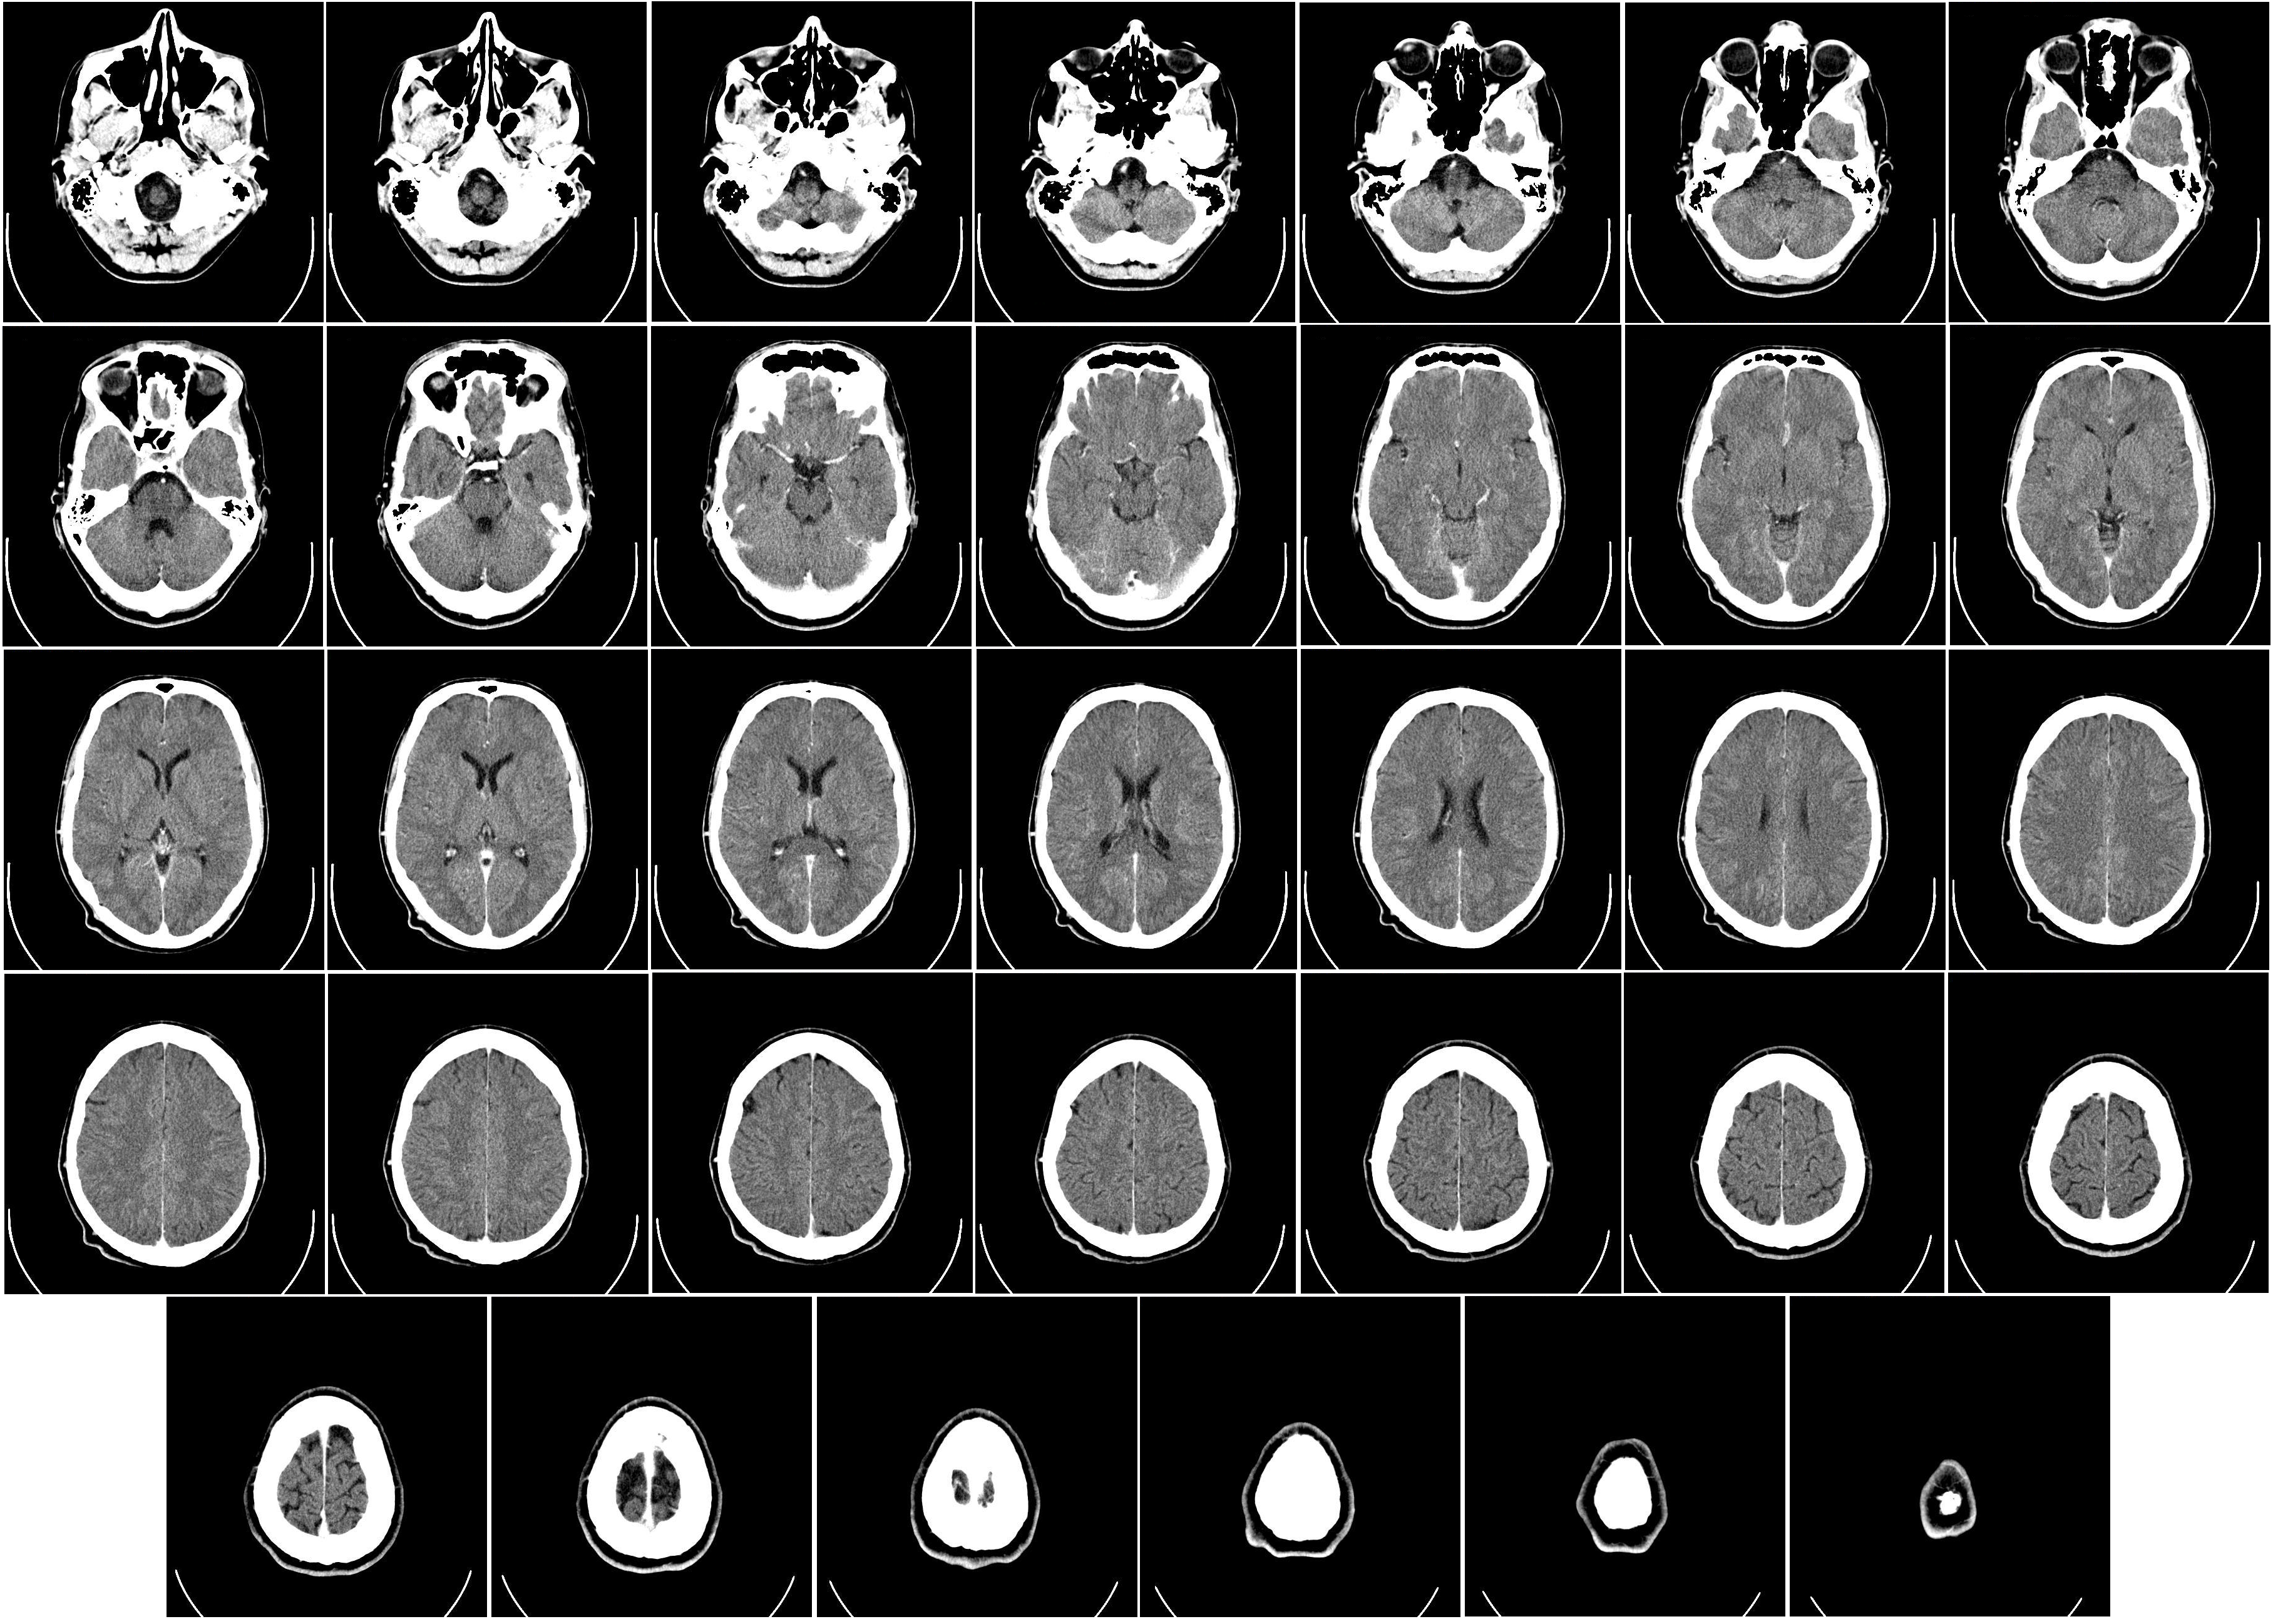
\includegraphics[width=0.5\textwidth]{Computed_tomography_of_human_brain}
\centering
\captionsetup{justification=centering}
\caption{Computed tomography of human brain, slice of 3D volume from base of the skull to top. Source: wiki}
\label{fig:ct_humna_brain}
\end{figure}

\noindent\\
Before creating 3D internal structure of the object, there are in between many steps which have to be performed. In order to make it simple, the example of CT machine can be considered. In CT machine, X-rays are used because it has ability to penetrate most of the objects. Using X-rays, many 2D projections are taken for the 3D object (in case of 2D object, 1D projections are taken) at different angles. These projections are also called as \textit{tomographic projections}. These tomographic projections are defined as \textit{Radon transform}. Then, by using all these 2D tomographic projections,  internal structure of 3D object is created.

\subsection{Tomographic Projection}\label{sec:tomo_pro}
For better understanding, consider 2D object and its 1D projection (figure \ref{fig:parallel_beam}) as it is much easier to understand. But, this concept can easily be extended for 3D objects and their 2D projections. For taking projection, a parallel beam of X-rays are fired on the object at some fixed angle ${\theta_k}$. The degree of absorption of X-rays by the object are recorded by the detector which is called as projection at angle ${\theta_k}$. Now mathematical equation for the projection can be formulated. Let 2D object be defined as $f(x,y)$. Then Projection at angle ${\theta_k}$ is given by

\begin{equation}
R(f) = g(\rho_j,\theta_k) = \int_{-\infty}^{\infty} \int_{-\infty}^{\infty} f(x,y) \delta(x\cos\theta_k+y\sin\theta_k - \rho_j)  dxdy
\label{eq:radon_trasform}
\end{equation}

\noindent
$R(f)$ is called as \textit{Radon transform} of function $f$. $g(\rho_j,\theta_k)$ is read as projection of $f(x,y)$ at angle $\theta_k$ and $\rho_j$ distance from origin.

\begin{figure}[H]
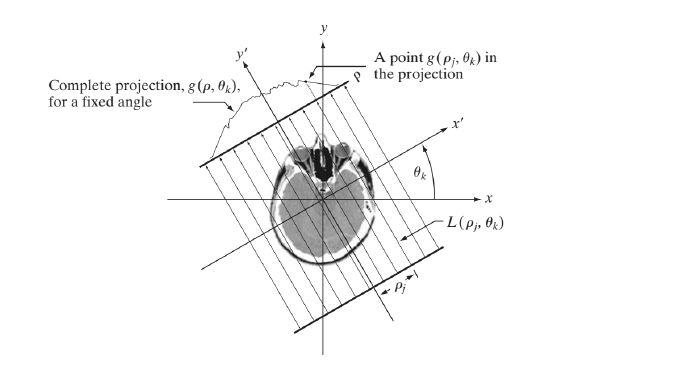
\includegraphics[width=1\textwidth]{parallel_beam}
\centering
\captionsetup{justification=centering}
\caption{ Parallel Beam (X-ray) Projection.\\ Source:Rafael C. Gonzalez , Richard E. Woods, Digital Image Processing}
\label{fig:parallel_beam}
\end{figure}


\subsection{Fourier Slice Theorem} \label{sec:for_slice_theorem}
Fourier Slice Theorem gives us the relationship between Fourier transform and Radon transform. Radon transform of $f(x,y)$ is given by eq. (\ref{eq:radon_trasform}). The 1D Fourier transform $g(\rho,\theta)$ w.r.t $\rho$ with fixed $\theta$ is given by eq (\ref{eq:ft_rt_1}).

\begin{equation}
G(\mu,\theta) = \int_{-\infty}^{\infty} g(\rho,\theta) e^{-j2\pi\mu\rho} d\rho
\label{eq:ft_rt_1}
\end{equation}

Now expanding the $g(\rho,\theta)$  and simplifying the equation

\begin{equation}
G(\mu,\theta) = \int_{-\infty}^{\infty} g(\rho,\theta) e^{-j2\pi\mu\rho} d\rho\\
\end{equation}

\begin{equation}
G(\mu,\theta) = \int_{-\infty}^{\infty} \int_{-\infty}^{\infty} \int_{-\infty}^{\infty} f(x,y)\delta(x\cos\theta+y\sin\theta - \rho)  e^{-j2\pi\mu\rho} dxdyd\rho \\
\end{equation}

\begin{equation}
G(\mu,\theta) = \int_{-\infty}^{\infty} \int_{-\infty}^{\infty} f(x,y) \bigg[ \int_{-\infty}^{\infty} \delta(x\cos\theta+y\sin\theta - \rho)  e^{-j2\pi\mu\rho} d\rho \bigg] dxdy \\
\end{equation}

\begin{equation}
G(\mu,\theta) = \int_{-\infty}^{\infty} \int_{-\infty}^{\infty} f(x,y) e^{-j2\pi\mu(x\cos\theta+y\sin\theta)} dxdy \enspace
\end{equation}


\begin{equation}\label{eq:ft_rt_2}
G(\mu,\theta) = \big[F(u,v)\big]_{u=\mu\cos\theta,v=\mu\sin\theta}
\end{equation}

\noindent
Here, $F(u,v)$ represents the 2D discrete Fourier transform of function $f(x,y)$. By eq (\ref{eq:ft_rt_2}) it can be concluded that, Fourier transform of projection of 2D object along some direction $\theta$ i.e $G(\mu,\theta)$ is equal to a slice of 2D Fourier transform of object along same direction $\theta$ in frequency plane, passing through origin. This is called as \textit{Fourier Slice Theorem} or \textit{Projection Theorem}. Similar theorem is also there for 3D object.

\subsection{Filtered Back Projection (FBP)}\label{subsec:reconst_fbp}
From section (\ref{sec:tomo_pro}) and (\ref{sec:for_slice_theorem}), it can be known how projections (tomographic projections) are taken and it's relation with Fourier transform of object. By exploiting these facts, the internal structure of the object can be reconstructed. Let us denoted 2D object as $f(x,y)$ and it's 2D F.T (Fourier transform) is represented as $F(u,v)$.

\begin{equation}\label{eq:inv_ft}
f(x,y) = \int_{-\infty}^{\infty} \int_{-\infty}^{\infty} F(u,v) e^{j2\pi(xu+yv))} dudv
\end{equation}

Let u=$\mu\cos\theta$ v=$\mu\sin\theta$,

\begin{equation}
f(x,y) = \int_{0}^{2\pi} \int_{0}^{\infty} F(\mu\cos\theta,\mu\sin\theta) e^{j2\pi(x\mu\cos\theta+y\mu\sin\theta))} \mu d\mu d\theta
\end{equation}

By using Fourier slice theorem eq (\ref{eq:ft_rt_2}) we get,
\begin{equation}
f(x,y) = \int_{0}^{2\pi} \int_{0}^{\infty} G(\mu,\theta) e^{j2\pi(x\mu\cos\theta+y\mu\sin\theta))} \mu d\mu d\theta
\end{equation}

After simplification we get,

\begin{equation}\label{eq:fbp}
f(x,y) = \int_{0}^{\pi} \int_{0}^{\infty} G(\mu,\theta) e^{j2\pi(x\cos\theta+y\sin\theta))} |\mu| d\mu d\theta
\end{equation}

\noindent
So eq (\ref{eq:fbp}) says that, if there are many projections at different angles then it can recover $f(x,y)$, i.e. object internal structure from projections. But, one concern is there i.e. in eq (\ref{eq:fbp}) $|\mu|$ (ramp filter) is an \textit{unbounded} function, therefore it is not integrable. In order to solve this problem Ram-Lak filter ($rect(\mu D)$) or Ram-Lak hamming filter is used. Updated FBP equation is given by eq (\ref{eq:fbp_ramlak}) using Ram-Lak filter.


\begin{equation}\label{eq:fbp_ramlak}
f(x,y) = \int_{0}^{\pi} \int_{0}^{\infty} |\mu| rect(\mu D) G(\mu,\theta) e^{j2\pi(x\cos\theta+y\sin\theta))}  d\mu d\theta
\end{equation}


\subsection{Reconstruction using Compressed Sensing}\label{subsec:reconst_cs}
In this section, another method for reconstruction using the set of projections taken at different angles is discussed. This method uses the concept of Compressed sensing (CS). CS works here because number of angles of projections are limited due to various reason like cost, energy and health considerations. This type of problem is also called as \textit{angle starved} problem. It is known that images are sparse or compressible in standard basis like DCT. So, CS based optimization equation for tomographic reconstruction is given by eq (\ref{eq:cs_eq1})

\begin{equation}\label{eq:cs_eq1}
E(\boldsymbol{\beta}) =  ||\boldsymbol{y - RU\beta}||^2 +\lambda||\boldsymbol{\beta}||_1
\end{equation}

\noindent
Here, $\boldsymbol{y}$ vector is created by concatenating 1D projections of various angles. $\boldsymbol{U}$ is the basis matrix in which image/object f(x,y) is sparse or compressible. $\boldsymbol{\beta}$ is the representation of ${f(x,y)}$ in $\boldsymbol{U}$ basis, i.e. ${f(x,y)}$ satisfy eq (\ref{eq:cs_spare_rep}). $\boldsymbol{R}$ is the Radon matrix (it can also be  Radon operator)

\begin{equation}\label{eq:cs_spare_rep}
vec(f)) =  \boldsymbol{U\beta}
\end{equation}

\noindent
Eq (\ref{eq:cs_eq1}) can easily be solved by using many optimization algorithm such as ISTA.  It is being observed that when number of angles are less then CS based reconstruction gives good result as compared to FBP up to certain limit.

\subsection{Application}
Tomographic reconstruction has many applications mostly in health care such as CT scan, industrial application such as fault detection in machines, observation of plant roots, remote sensing i.e. observing underground objects or phenomena and most importantly study of protein, bacteria, Ribosome, cells and virus by biologist for creating medicine or vaccination or for any other purpose.

\section{Tomography under unknown viewing parameters }
In previous section (\ref{sec:tomo_recons}), reconstruction from projections was considered where angle at which each projections were taken were  known. But if only projections are known but not angles then, previously seen method for reconstruction will not be applicable. 

\noindent
There are various application where angles are not known such as patient moving during CT scanning (this mostly happens in pediatrics CT), geometric errors in CT machine \cite{malhotra2017signal}, moving insect tomography, cryo-electron tomography and many more. In all these cases, the projection angles of the available projections are unknown. Moreover in cryo-electron microscopy the shifts of the projections are also unknown. Therefore, this is termed the problem of \textit{tomography under unknown viewing parameters}.

\noindent
This section talks about reconstruction of internal structure of object back from projection when angles are not known i.e. only with the help of tomographic projections.

\subsection{Moment Based Reconstruction}\label{subsec:recont_moment-based}
Again, for simple understanding, lets consider 2D object and it's 1D projection. But this logic can easily be extend for 3D object and it's 2D projection.

\noindent
Let say f(x,y) be the object then, moment of order (p,q) for f(x,y) is given by eq (\ref{eq:moment_pq}).

\begin{equation}\label{eq:moment_pq}
\boldsymbol{M}_{p,q} =   \int_{-\infty}^{\infty}  \int_{-\infty}^{\infty} f(x,y) x^py^q dxdy
\end{equation}

\noindent
Let $P_\theta(s)$ be the projection at angle $\theta$ then moment of order (n) is given by eq (\ref{eq:moment_proj})

\begin{equation}\label{eq:moment_proj}
\boldsymbol{M}_{\theta}^{(n)} =   \int_{-\infty}^{\infty} P_\theta(s) s^n ds
\end{equation}

where,

\begin{equation}\label{eq:proiection_p(s)}
P_\theta(s) =   \int_{-\infty}^{\infty} \int_{-\infty}^{\infty} f(x,y) \delta(x\cos\theta+y\sin\theta - s) dx dy
\end{equation}

\noindent
Therefore, by substituting $P_\theta(s)$ in eq(\ref{eq:moment_proj}) by eq(\ref{eq:proiection_p(s)}) and after simplification,

\begin{equation}
\boldsymbol{M}_{\theta}^{(n)} =   \int_{-\infty}^{\infty} \int_{-\infty}^{\infty} f(x,y) (x\cos\theta+y\sin\theta)^n dxdy
\end{equation}

\noindent
So, the Helgasson Ludwig Consistency Conditions (HLCC) \cite{malhotra2016tomographic} \cite{basu2000feasibility} \cite{natterer1986mathematics} gives us the relation between the image moment and its projection moment which is given by eq(\ref{eq:moment_proj_img}).

\begin{equation}\label{eq:moment_proj_img}
\boldsymbol{M}_{\theta}^{(n)} =  \Sigma_{l=0}^n f(x,y) \boldsymbol{C}_n^{n-l} (\cos\theta)^{n-l} (\sin\theta)^l \boldsymbol{M}_{n-l,l}
\end{equation}

\noindent
Here, projections of the f(x,y) is known. So it's moment i.e $\boldsymbol{M}_{\theta}^{(n)}$. By eq(\ref{eq:moment_proj_img}) unknown angles can be found out by iteratively solving for angles \cite{malhotra2016tomographic}.Once the angles for these projections are found then any of the earlier mentioned methods for reconstruction can be applied. \\

\noindent
Advantages of this method are simple to implement, makes direct use of consistency conditions and work well for small number of angles. But, major drawback of this method is that it is highly sensitive to noise.

\subsection{Order Based Reconstruction}\label{subsec:recont_order-based}
This method is very much similar to machine learning based method. In this, all acquired projections are sorted i.e. in order of increasing angles. Only issue is that this method requires large number of projection and it assumes that all unknown projection angles are independently sampled from uniform distribution, also angles can be from any known distribution but then accordingly algorithm will change. Assuming distribution to be uniform, then this problems reduce to matching problem where we have to match each projection to one of the angles sampled evenly from unit circle.\\

\noindent
It's an iterative algorithm, where initial projection say $P_0$ and one angle say $\theta_0$ are chosen. Then, $P_0$ projection is mapped with angle say $\theta_0$. After that, find the closest projection to $P_0$ and then that projection is mapped with next angle from sorted distribution. This process is repeated till full mapping is completed. \\

\noindent
Once it finds the angles for all projections then apply any of the earlier mentioned method for reconstruction. 

\chapter{Introduction to Cryo-EM}
\section{Motivation}
There are many applications where tomography concept is being used such as CT in which X-Rays are used. Suppose biologist wants internal 3D model of a protein particle. Then, for this type of problem, CT machine cannot be used because it is niether designed for it nor a light-microscope. It is designed for viewing surface. Since late 20th century, a method called as \textit{X-ray Crystallography} is being used for this kind of problem when sample (object under study) is very tiny\cite{wang2017cryo_crystal}. 

\noindent\\
Next section talks briefly about \textit{X-ray Crystallography} and problem faced in it. Also the benefit of \textit{Cryo-EM} over X-ray Crystallography.

\subsection{X-ray Crystallography}
As the name suggest, X-ray is being used for taking projections of tiny particle like protein or DNA. It uses the Braggs's law of \textit{X-ray diffraction} by crystal for taking the tomographic projection \cite{wang2017cryo_crystal}. Here, in figure (\ref{fig:xray-diffraction}), DNA sample is firstly crystalline and then  placed in between focused X-ray beam and detector. Because of crystal, X-rays are diffracted and this diffraction is captured on the detector screen. Then, from the recorded reading model reconstruction is done.

\begin{figure}[H]
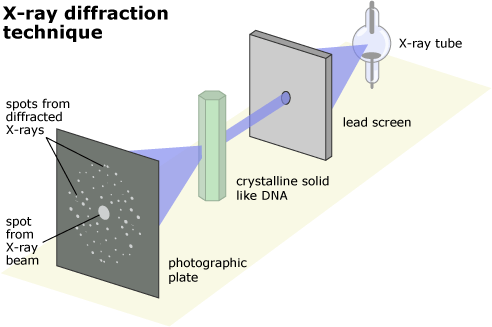
\includegraphics[width=0.75\textwidth]{xraydiffraction}
\centering
\captionsetup{justification=centering}
\caption{ X-ray Diffraction.\\ Source: undsci.berkeley.edu - article-dna 04}
\label{fig:xray-diffraction}
\end{figure}



\subsection{Cryogenic Electron Microscopy (Cryo-EM) }
Cryo-EM uses the electron beam for taking projections. Because of that, resolution of cryo-em is much better than X-ray crystallography. Depending on the type of sample under study, power of electron dose is set 
to get maximum possible resolution for that sample \cite{diebolder2012pushing}. Here, the procedure for sample creation is completely different from X-ray crystallography. Firstly, a slice of sample to study is placed in vitrified water (water with some amount of ethane) and then freeze below \ang{-150}C \cite{diebolder2012pushing} \cite{wang2017cryo_crystal}. After that slide is placed in electron microscopy (EM) and observations/projections are made in cryogenic conditions. As whole thing is carried out in cryogenic conditions and appliance used is Electron-Microscope (EM) that's why this is called \textit{Cryo-EM}. See figure (\ref{fig:xray_crystal_cryoem}) for working of Cryo-EM.

\begin{figure}[H]
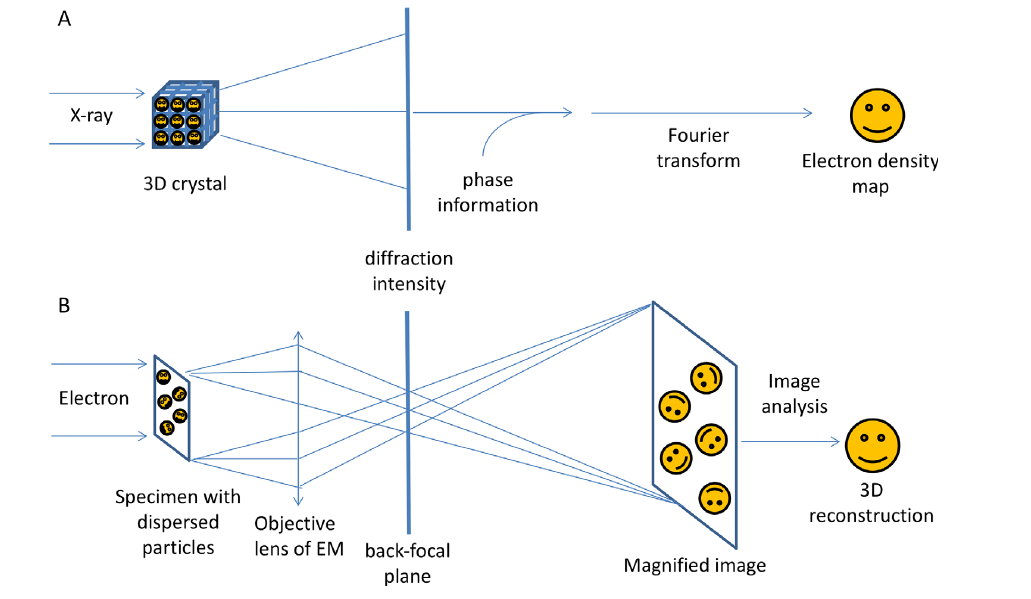
\includegraphics[width=0.75\textwidth]{xray_crystal_cryoem}
\centering
\captionsetup{justification=centering}
\caption{ Functional difference between X-ray crystallography (A) and single particle cryo-EM (B) Source: Wang et al. \cite{wang2017cryo_crystal}}
\label{fig:xray_crystal_cryoem}
\end{figure}

\noindent
X-ray crystallography resolves structures of macro-molecules at atomic level. But, cryo-em can provide structural information at resolution from 3\text{\AA} to $~$3nm. As cryo-em sample creation doesn't want sample to be in crystalline form so it can also examine non-crystalline structure. Also, it reveals the structure  closer to its native state than X-ray crystallography \cite{wang2017cryo_crystal}. See figure (\ref{fig:xray_crystal_cryoem}) for working difference of both methods.

\section{Basic Pipeline}\label{sec: basic_pipeline}
This section talks about cryo-em whole base pipeline starting from selecting the particle from micrograph (image (b) \ref{fig:micrograph}) also called as \textit{particle picking} generated from Cryo-EM to it's 3D model reconstruction (similar to image (a) \ref{fig:micrograph}). 

\begin{figure}[h]
\centering
\begin{subfigure}{.5\textwidth}
\centering
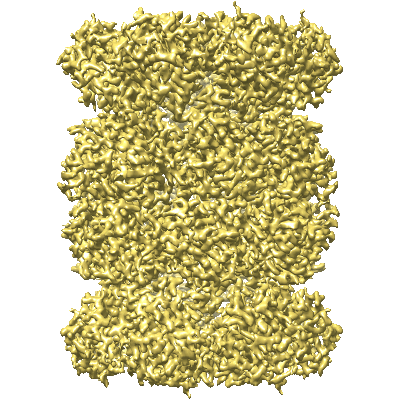
\includegraphics[width=0.5\linewidth]{EMPIAR-10025}
\captionsetup{justification=centering}
\caption{T20S Proteasome}
\end{subfigure} %

\begin{subfigure}{.75\textwidth}
\centering

\includegraphics[width=0.75\linewidth]{micrograph}
\captionsetup{justification=centering}
\caption{ Micrograph of T20S Proteasome at 2.8 \text{\AA} Resolution Source: EMPIAR-EBI data-bank}
\end{subfigure}
\caption{ Source: EMPIAR-10025 EBI data-bank: https://bit.ly/2JrFCD5}
\label{fig:micrograph}
\end{figure}

\subsection{Particle Picking}
Cryo-EM gives micrograph of very large size example 7000x7000. These micrographs contain lots of radon projections of the sample (around in thousands) taken by parallel beam because EM shoots electron beam in parallel. For reconstruction process, the very first steps is to manually or automatically mark out these projections by drawing bounding box around particles or just by marking its center in micrograph (\ref{fig:pp_from_micrograph}) and then crop out these projections. After that all the cropped out projections are collected into \textit{stack} of projection images. As micrograph is very huge and it contains large amount of projections, so manually marking is very time consuming process. Now a days, biologist crowd source this initial phase of particle picking \cite{bruggemann2017exploring}. But, even after crowd sourcing, they have to remove wrongly marked particle by themselves which is still a very time consuming activity.  

\begin{figure}[h]
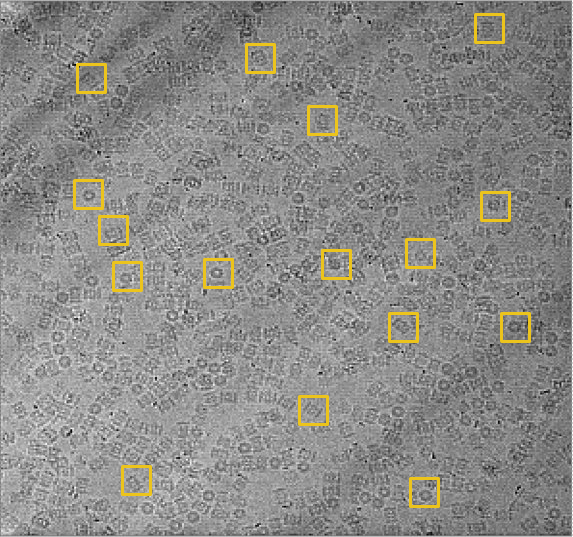
\includegraphics[width=0.75\textwidth]{micrograph_pp_10025}
\centering
\captionsetup{justification=centering}
\caption{ Manual particle picking from micrograph of T20S Proteasome Source: EMPIAR-10025 EBI data-bank\protect\footnotemark} 
21

\label{fig:pp_from_micrograph}
\end{figure}
\footnotetext{\label{fn:empair-1005databank}EBI data bank: http://www.ebi.ac.uk/pdbe/emdb/empiar/entry/10025/}

\noindent\\
For saving time in particle picking, there are few automated and semi-automated algorithms. Example for one such automated algorithm is "difference of Gaussian" where a broad 2D Gaussian function (i.e. having large $\sigma$) convolved with micrograph is subtracted from narrow 2D Gaussian function (i.e. having smaller $\sigma$) convolved with micrograph. Result of this method gives circular white object pattern  with a dark surrounding \cite{sigworth2016principles}. Problem with this approach is the tuning of hyperparameters like here, $\sigma$ depending on the type particles and noise level in micrograph. An example of semi-automated method is a machine learning based particle picking \cite{chen2012detection}. In case of machine learning, classifiers are trained in same noisy environment as of micrograph and tested on the same noisy environment. The next chapter talks about some semi-automated method and new detector design and it's experimental results on simulated data.

\subsection{CTF correction}
Image formation in Cryo-EM for biological samples taken under cryogenic environment by freezing the sample in vitrified water can mathematically be described as Contrast Transfer Function (CTF). CTF depends on many parameters such as defocus, astigmatism, beam coherence, energy spread and tilting of the sample \cite{diebolder2012pushing}. CTF oscillates rapidly, with some Fourier components transferred with positive contrast and other with inverted contrast. CTF is directly proportional to defocus i.e. if defocus increases then density of reversal increases which means higher contrast. So if defocus is higher, it helps in visualizing micrograph which further helps in marking of the particle and determining its orientation. But, this high defocus give rise to astigmatism i.e circular ring in CTF turns into  ellipse \cite{sigworth2016principles}. Because of all these issues, \textit{CTF correction} is needed for the micrograph.  

\subsection{Clustering}\label{subsec:clustering}
The projection image from the \text{stack} of images is highly noisy i.e. it has very low SNR value since the electron beam used for taking projection is of very low power otherwise it will damage the sample. Also, distortion due to CTF effects makes it difficult to evaluate the projection. So, in order to resolve this problem, \textit{clustering} of all projections from stack are done. After the clustering, all projections within a cluster are averaged out to get one average projection per cluster. This helps a lot in reducing the noise.   


\begin{figure}[h]
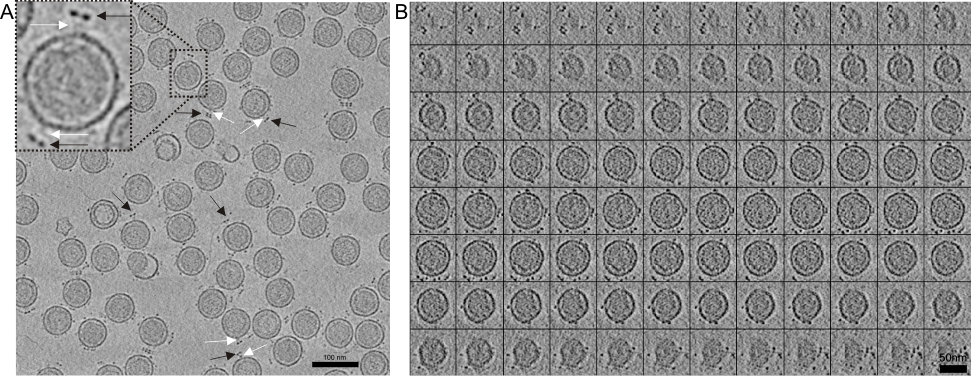
\includegraphics[width=1\textwidth]{phi-12-slices_clustering}
\centering
\captionsetup{justification=centering}
\caption[Clustering]{a) Phi12 bacteriophage micrograph b) Each row represent similar projection. Showing cluster of of projection before averaging.\\Source: med.nyu.edu \protect\footnotemark}
\label{fig:clustering}
\end{figure}
\footnotetext{\label{fn:empair-1002databank}EMPIAR-1002 data bank: https://med.nyu.edu/skirball-lab/stokeslab/phi12.html}

\noindent\\
There are lots of methods for performing clustering. Algorithm used by RELION (REgularized LIkelihood OptimizatioN) uses \text{maximum likelihood 2D classification}, it is a very widely used software tool which performs all the base pipeline task \cite{scheres2012relion}. In brief, this algorithm firstly select an initial set of reference projections. Then, for each projection, probability w.r.t rotation and translation with each reference projection is calculated. Then averaging is carried out for projections with higher probabilities. Averaged projections are then taken as new reference projections and the whole process is repeated few times.

\subsection{Angle Assignment}
After clustering (section \ref{subsec:clustering}) step, projections are little noise free and CTF correction has been done up to certain level because of averaging. Now, 3D model is reconstructed using these projections, but for 3D reconstruction, there is a need of angles at which these projections are taken if reconstruction is done using method discussed in previous section i.e. FBP (\ref{subsec:reconst_fbp}) or CS (\ref{subsec:reconst_cs}). Finding angles and then reconstruction is called as \text{tomography under unknown angle}. So angles can be found out using  two methods i.e. Moment-based (\ref{subsec:recont_moment-based}) and Order-based (\ref{subsec:recont_order-based}).

\subsection{3D Reconstruction}
Once angles for each projection are known then 3D reconstruction is possible using FBP (\ref{subsec:reconst_fbp}) or CS (\ref{subsec:reconst_cs}) based method. As always, if there are variety of projections at different angles then 3D reconstruction will be more accurate. But in \textit{SPR (single particle reconstruction)} \cite{sigworth2016principles} many times getting projections at various  angles is not possible because of the particle orientation as projection angle of EM is fixed i.e. perpendicular to slide. In EM, slide is the place where sample is placed for observation or projection. So the only way to get projections at different angles is from particles orientation in frozen vitrified water sample \cite{diebolder2012pushing}. But problem is that particles orientation in sample is not fully random. So there will always be the case in which projection can not acquired along certain direction. For solving this problem, biologist tilt the sample slide with some angle and then projection are taken. This tilting is done many times in many direction to cover large possible directions. If projections are taken this way, then effect of CTF will be different for different tilt direction and also within slide because of tilt. In this type of situation CTF correction is more challenging \cite{diebolder2012pushing}. This method is called as \textit{Cryo-EM Tomography}.

\section{Challenges}
\subsection{Radiation damage}
In Cryo-EM, electron beam is used. Problem with it is that these electron start interacting with the sample electron. In other terms, if the exposure time of vitrified biological sample is increased then this leads to breaking of covalent bonds of sample (because of electron-electron integration) and progressively it will do the structural degradation\cite{diebolder2012pushing}. Therefore, total dose of electron that can be used is limited. This also affects the resolution i.e. magnification of cryo-em which means depending on the biological sample under study, resolution will be different.

\subsection{Noise}
Higher power electron dose usually destroys the sample. So, for handling these kind of issues, low power electron doses are used. But, this leads to increase in noise w.r.t. signal i.e. SNR for the micrograph become very low. In Cryo-EM, the distribution of noise is \textit{Poisson distribution} defined by eq (\ref{eq:poisson_dist}), which makes the problem more challenging as Poisson noise is signal dependent. In case of Image I(x,y), it is given by equation eq (\ref{eq:poisson_noise}) which means removal of Poisson noise is far more challenging than signal independent noise (like i.i.d Gaussian noise)  

\begin{equation}\label{eq:poisson_dist}
    P(X=i) = \frac{\lambda^i}{i!} e^{-\lambda}
\end{equation}

\begin{equation}\label{eq:poisson_noise}
    \begin{aligned}
        Y(x,y) &  \sim \textrm Poisson(I(x,y))\\
    \end{aligned}
\end{equation}

Y(x,y) represent Poisson-noisy version of I(x,y).\\

\subsection{Unknown angles}
When projections are taken in cryo-em, angle at which beam is fired is known, but problem here is that when biological samples are frozen in vitrified water, then orientation of these samples are random. So, even if the angel at which beam is fired is known, the projection angles are different for every particle because of their orientation. As orientation of these samples are random which also means projection angles are also unknown, this information lose causes problem at the time of reconstruction from these projections.

\subsection{Heterogeneity}
Sample of same biological particles many not be identical i.e. every particle has some heterogeneity associated with it. Because of this complexity in whole process increases. At the time of selecting particle from micrograph, one has to make sure that consistency of particle has been marked otherwise this causes problem at the time of finding angles and also it might give rise to wrong 3D structure reconstruction \cite{sigworth2016principles}.

\subsection{Manual Particle Picking}
Picking of particle is mostly time consuming and an important task. As discussed previously, wrong particle picking will lead to wrong result. Still today, many prefer to mark these particle in micrograph with hands so that error in particle picking can be reduced.   

\noindent\\
So, by the nature of problem, there is a need of robust automatic or semi-automatic algorithm for particle picking which can handle outlier like few wrongly marked particle. Also, these algorithms should be fast at the time of finding the particle location in micrograph. The next chapter is mostly focused on first stage of the pipeline i.e. \textit{particle picking} and will talk about few semi-automated methods and their testing on simulated data set.  

\section{Nobel Prize}
In the year 2017, Jacques Dubochet, Joachim Frank and Richard Henderson shared the \textit{Nobel Prize in Chemistry} for developing a technique to image biomolecules. There work helps researchers to see biomolecules look in 3D. In 1970, Richard Henderson, a molecular biologist was trying to determine the shape of a protein called bacteriorhodopsin but X-ray Crystallography was not working because of the issue with structure bacteriorhodopsin. Then they used electron microscope for the first time for biological particle and produced their first 3D model of the protein. During same period Joachim Frank developed image-processing software to make sense of the fuzzy pictures that are produced when an electron microscope is aimed at a protein, and to convert these two-dimensional blurs images into 3D molecular structures. Also in the early 1980s, Jacques Dubochet worked out how to prevent water-soluble biomolecules from drying out in the vacuum of an electron microscope and  his team found a way to flash-freeze solutions of proteins using liquid ethane, keeping the molecules relatively still when they were analyzed under electron microscope. There research during the period 1970s-1980s has benefited researchers in analyzing biomolecules in 3D because of that in the year 2017 they got Nobel Prize in Chemistry.

\chapter{Particle Picking using Machine Learning}
\section{Semi-Automated Method}
In semi-automated procedure, there is some need of human intervention in the procedure. This chapter talks about such type of semi-automated method for particle picking. All methods discussed here require only one time human intervention and that even at the start of method such as training of \textit{Support Vector Machine (SVM)} classifier. Here, human will mark out few projections manually on micrographs say around 2K (far less than 30K) and then these projections are given as input to machine learning based classification algorithm which then try to distinguish between particle and background.


\section{Training Architecture}\label{sec:train_arch}

\begin{figure}[H]
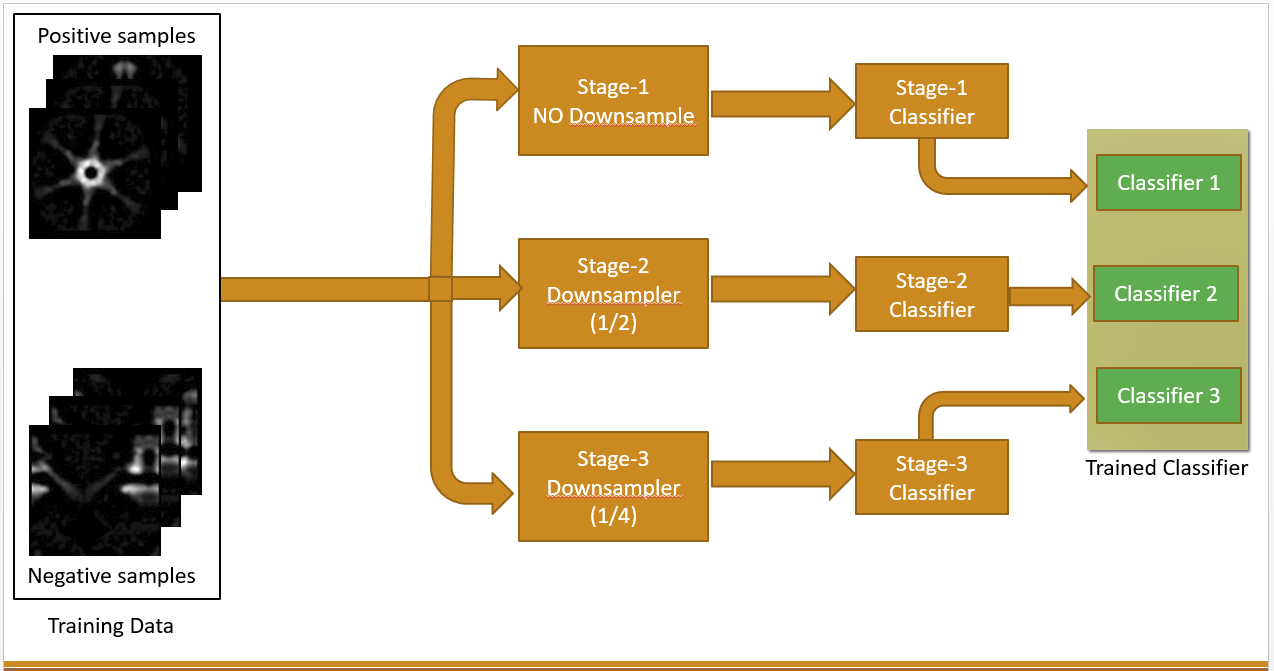
\includegraphics[width=1\textwidth]{train_arch}
\centering
\captionsetup{justification=centering}
\caption{Particle Detector Training Architecture}
\label{fig:training_arch}
\end{figure}

One simple way to train machine learning classifier is to feed training set to the SVM classifier and tune the hyper-parameters which are best suited for the application. Then, use that trained classifier for detection purpose. But, this architecture of training will not work in cryo-em  micrograph because actual micrograph dimensions are in the thousands example 7000x7000 or much bigger than this. In our experiment, the dimension of micrograph is 7420x7670 (~ 56 million pixels). So, if simple architecture is used then time required for creating \textit{probability map} ( some also calls it \textit{score map} or \textit{heat map}) for micrograph will be huge. Probability of a patch centered at $\boldsymbol{x_i}$ $(x_i,y_i)$ for a positive class is calculated using per class score generated by SVM  (our case only classes) and softmax function. For two class, softmax is given by eq(\ref{eq:softmax}).

\begin{equation}\label{eq:softmax}
    P(y=+ve | \boldsymbol{x_i}) = \frac{e^{si_{+ve}}}{e^{si_{+ve}}+e^{si_{-ve}}}
\end{equation}

\noindent\\
Here, $si_{+ve}$ and $si_{-ve}$ are the class scores generated by SVM model for patch centered at $x_i$. Scores are inversely related to the distance from  the separating hyperplane. 

\noindent\\
For example, take micrograph of dimension $2000\times2000$ i.e. $4\times10^6$ pixels. Let us say, already trained classifier takes $0.001$ sec for classifying one patch of dimension 333x333 centered at ith pixel and give its probabilistic score. Then, for finding score at every pixel will take around 40000 secs ($4\times10^6\times0.001$) which is approximately equals to 11hrs which means that this is a very poor particle picker as expected time should be in seconds or up to minutes but not in hours.


\noindent\\
In order to overcome this problem, the new architecture (by tweaking the current way of training) follows downscaling of model i.e. in case of \textit{3-downscale} model three classifiers are trained.  The first classifier is simple one i.e. no downscaling, the second model train classifier at downscale of 2 and the third model at downscale of 4. So, once the whole training process in completed, output will be \textit{3-trained-classifiers} in case of 3-downscale model. Figure (\ref{fig:training_arch}) shows the training architecture of 3-downscale model.

\noindent\\
Depending on the size of the micrograph, the architecture code can be increased or decreased (just by changing configuration file) considering computation time and accuracy of the system. 

\section{Particle Detector Architecture}\label{sec:detector_ach}

\begin{figure}[H]
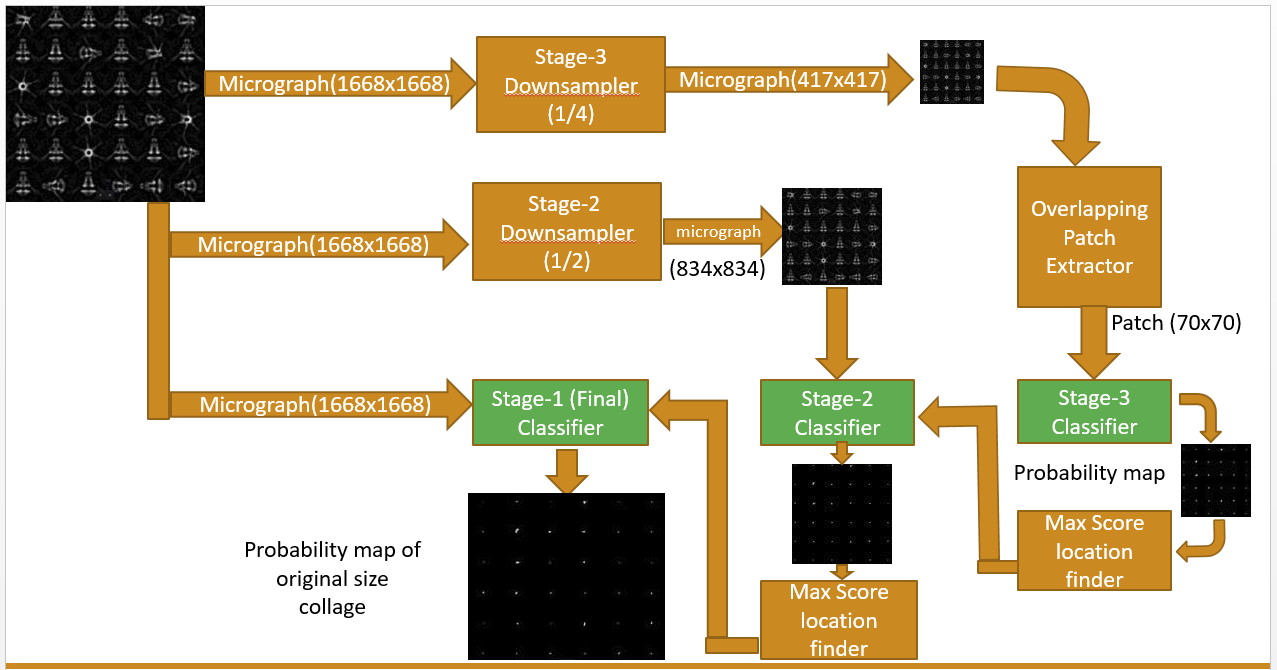
\includegraphics[width=1\textwidth]{test_arch_1}
\centering
\captionsetup{justification=centering}
\caption{Particle Detector}
\label{fig:test_arch}
\end{figure}

Detecting particle in the micrograph and creating its probability map will take huge amount of time in case of single classifier, see section (\ref{sec:train_arch}) for its computation time. In order to reduce this detection time, the new training architecture has been proposed i.e. \textit{downscale} model. The detection using this new trained model is little complex as compared to a  \textit{new trained modelled architecture}. Figure (\ref{fig:test_arch}) describes the work flow of detection process.

The detection process is a reverse training process in terms of stages. In case of 3-downscale model, firstly stage-3 is performed then stage-2 and at last stage-1 i.e. in reverse order. Stage-3 has only one input i.e. the original micrograph is downsampled by 4 and remaining i-1 stage will have 2 inputs i.e. for stage-j ($j<3$) one input will be micrograph downsampled by $2^{j-1}$ and the other input will the output of (j+1)th stage passed through "Max score location finder" function. "Max score location finder" finds all the (x,y) coordinates in the probability map which are having probability values more than certain \textit{min-threshold} (default 0.8). Min-Threshold has to be set depending on how well a classifier is being trained.  Apart from nth stage (here 3rd) remaining stages do not run on every pixel. They use the location given by the previous (j+1)th stage. After up scaling these locations, their 4 point neighbour probabilistic score is calculated using input micrograph at that stage using that stage classifier. 


Our code also supports three execution modes. These are single CPU, CPU Pooling and GPU. The computational table (\ref{tbl:computation_tbl}) shows time for getting probability map of a micrograph dimension of 1998x1998 three modes.

\begin{center}
\begin{table}[H]
    \begin{tabular}{||c|c|c|c||} 
        \hline \hline
      -     & Single CPU & 12-CPU Pool & GPU \\ [0.5ex] 
        \hline\hline
        Our Arch Time & $\thicksim$ 1.15 hrs & $\sim$ 9 mins & $\sim$ 4mins \\ \hline
        Simple Arch Time & Not worth computing&  16.97 hrs (61100 sec)  & - \\ 
        \hline
        \hline
    \end{tabular}
    \caption{Computation Table}
    \label{tbl:computation_tbl}
\end{table}
\end{center}


\section{Classifier}
This section talks about three classifiers, first is \textit{SVM} , second is \textit{Random Forest} and last one uses deep learning which is \textit{Faster R-CNN}. The next section will discuss about the experimental results when these classifiers are used for particle picking.

\subsection{Support vector machine (SVM) }
Support Vector machine is a machine learning algorithm used for classification. In our case, only two classes are there, one is positive class (i.e. true projection) and  another is negative class. Also, as compared to deep learning, it requires far less data points to train. 

SVM tries to optimize following objective function eq (\ref{eq:svm_obj_fun}).
Let $y^i$ be the true label of $\boldsymbol{x}^i$ data point. In our case, as only two classes are there, so $y^i$ will be 1 for positive image and -1 for negative image. In eq(\ref{eq:svm_yi}), $\boldsymbol{b}$ is bias term (unknown), $\phi(\boldsymbol{x})$ is a feature function i.e. for given input data point $\boldsymbol{x}$, it returns features vector and  $\boldsymbol{w}$ is weight vector which classifier learns along with $\boldsymbol{b}$. $\xi_i$ represent the slackness condition. In case of SVM, $\xi_i$ is used when there is no perfect separability of the data point. 

\begin{equation}\label{eq:svm_yi}
    y^i= \boldsymbol{w}^T \phi(\boldsymbol{x^i}) + \boldsymbol{b}
\end{equation}


\begin{equation}\label{eq:svm_obj_fun}
  \begin{aligned}
    \boldsymbol{(w^*,b^*)} = & \enspace argmin_{w,b} \enspace \frac{||w||_2}{2}\\  
     &\enspace  subject \enspace to,\\
     &\enspace y^i(\boldsymbol{w}^T \phi(\boldsymbol{x^i}) + \boldsymbol{b}) \geq 1-\xi_i\\
      &\enspace \xi_i \geq 0 \enspace  \forall i = 1,2 \cdots , n 
  \end{aligned}
\end{equation}

For better classification, $\phi(.)$  places a vital role. $\phi(.)$ is not learned during training, it should be known before hand. In order to solve this problem, there is an alternate representation of SVM classifier i.e. using Kernel function $\boldsymbol{K(.,.)}$. Kernel representation do not use $\phi(.)$ and it is given by eq (\ref{eq:svm_kernel_obj_fun}). In eq(\ref{eq:svm_kernel_obj_fun}) $y_i$ is the class label of the datapoint $x_i$, $\boldsymbol{K(.,.)}$ is the kernel function and C is the hyperparameter.

\begin{equation}\label{eq:svm_kernel_obj_fun}
  \begin{aligned}
     \max\limits_{\alpha} & \enspace \frac{-1}{2} \sum\limits_i^n \sum\limits_j^n \alpha_i \alpha_j \boldsymbol{K(x_i,x_j)}  + \sum\limits_i^n \alpha_i \\
     &\enspace  subject \enspace to,\\
     &\forall \alpha_i \epsilon \big[0,C]\\
     &\sum\limits_i^n \alpha_i y_i = 0\\
  \end{aligned}
\end{equation}

\subsection{Random-Forest}
\textit{Random-Forest} is a variant of \textit{Decision-Tree}. Random-Forest has ensemble of trees (see figure \ref{fig: Random-Forest} ) whereas Decision tree has single tree. Each tree of Random-Forest is constructed in the same way as Decision-Tree. Only difference is that tree is constructed for \textit{random} subset of dataset and features.

\begin{figure}[H]
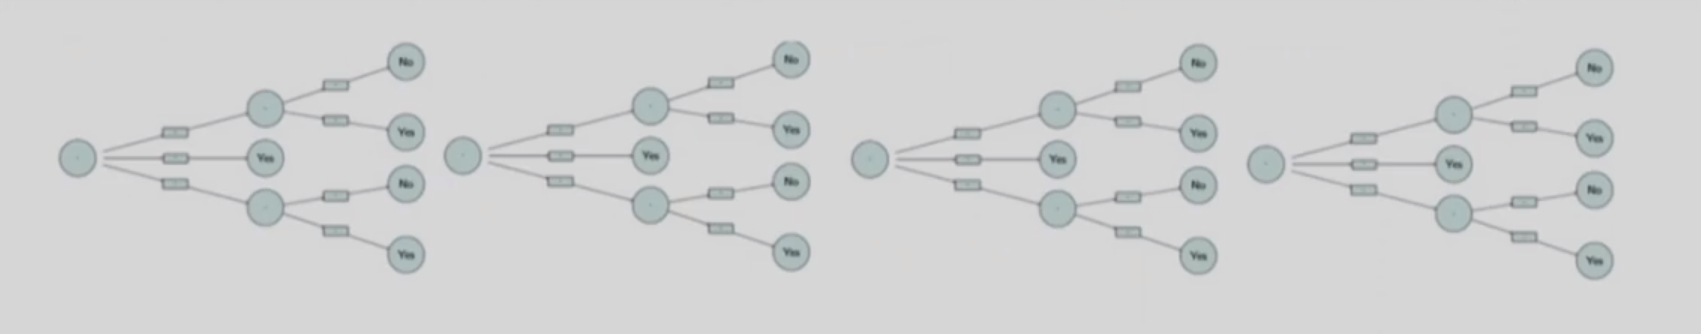
\includegraphics[width=1\linewidth]{random-forest.png}
\centering
\captionsetup{justification=centering}
\caption{Random Forest. Circular nodes are features and rectangles are thre attributes of their respective features. Source: CS725 IIT-Bombay: Lecture-25 by Prof. Ganesh Ramakrishnan}
\label{fig: Random-Forest}
\end{figure}

Below is the \textit{Bagging} algorithm for constructing Random-Forest. Bagging stands for "\textbf{B}ootstrapping \textbf{Agg}regat\textbf{ing}".  Let \textbf{B} be the number of trees to be constructed, \textbf{D} denotes complete dataset, $\boldsymbol{\phi}$ denotes complete features set of dataset \textbf{D} and $\boldsymbol{T}={}$ be the Forest set (initially empty).  In Bagging, each tree has equal weightage i.e 1 but in Boosting, each tree as different weightage. Also, in Bagging, each trees are independent of each other because of that these can be constructed parallely.

\subsubsection{Random-Forest Algorithm:} \label{subsec: Random-Forest}
\begin{enumerate}
  \item Uniformly at random (with replacements), sample subsets $\boldsymbol{D_s} \subseteq \boldsymbol{D}$ of the training data, $\boldsymbol{\phi_s} \subseteq \boldsymbol{\phi}$ of the feature set. 
  \item  Using $\boldsymbol{D_s}$ and $\boldsymbol{\phi_s}$, construct Decision-Tree $Ts$ using \textit{Decision-Tree Algorithm}.
  \item Repeat the step 1 and 2 for B times and keep adding the tree $Ts$ into the forest set $\boldsymbol{T}$.
\end{enumerate}

\subsubsection{Decision-Tree Algorithm:}\label{subsec: Decision-Tree}
Let S is a sample of training examples,  $p_{ci}$ is a proportion of examples with class $C_i$ (feature) in S and K be the number of class.
\begin{enumerate}
    \item Find $\phi^*$ $\leftarrow$  The \textbf{best} decision feature for next node
    \begin{enumerate}
        \item Entropy measures impurity of $S$: 
            \begin{equation}
                H(S) =  \Sigma^{K}_{i=1} - p_{ci} \log_{2} p_{ci}
            \end{equation}
        \item For class $\phi_i$, \textit{Gain} is defined by below equation. $ Gain(S,\phi_i )$ means expected Gain due to choice of $\phi_i$
            \begin{equation}
                Gain(S,\phi_i ) = H(S) - \Sigma_{v \in Values(\phi_i)} \frac{|S_v|}{|S|} H(S_v)
            \end{equation}
        where, $S_v$ means set of all examples having value of feature $\phi_i$ as v.
        \item Therefore, best $\phi^*$ feature for given S is define below equation.
             \begin{equation}
                \phi^*  =  argmin_{\phi_i} G(S,\phi_i)
            \end{equation}
    \end{enumerate}
    \item Assign $\phi^*$ as the decision feature for the node
    \item For each value (attribute) of $\phi^*$, create new descendant of node
    \item If training examples perfectly classified. Then STOP, Else iterate over new leaf nodes i.e. for each leaf node repeat the steps 1,2 and 3 recursively.
\end{enumerate}

Each tree of the Random-Forest is a week tree having very high variance and low bias. During testing, final result is calculated by averaging the results of all the B trees (see eq. \ref{eq: random-forest_avg_eq}) because of this final variance of the model goes down as they get canceled out. Probabilistic  score of new test point $\boldsymbol{x}$ is given by equation \ref{eq: random-forest_avg_eq}.

\begin{equation}\label{eq: random-forest_avg_eq}
        Pr(c|\boldsymbol{x}) = \frac{1}{|B|} \Sigma^{B}_{t=1} Pr_t(c|\boldsymbol{x})
\end{equation}
where $Pr(c|\boldsymbol{x})$ means probability of $\boldsymbol{x}$  belonging to class c and $\sigma$ is over all the trees of the Random-Forest.

\subsection{Faster R-CNN}
Faster R-CNN \cite{ren2015faster} is the  faster version of \textit{Fast R-CNN} \cite{girshick2015fast}. R-CNN stands for Region based Convolution Neural Network. R-CNN is the multiple object detector (localization and classification) which is the prior version of Fast R-CNN. The major difference between R-CNN \cite{girshick2014richrcnn} and Fast R-CNN \cite{girshick2015fast} is that Fast R-CNN has ROI (Region of Interest) pool layer with fully connected neural network for classification and regression (localization) but, in case of R-CNN  there is no concept of ROI, also SVM is used for of classification and CNN for regression.  See figure \ref{fig: R-CNN} for R-CNN and figure \ref{fig: Fast R-CNN} for Fast R-CNN.


\begin{figure}[H]
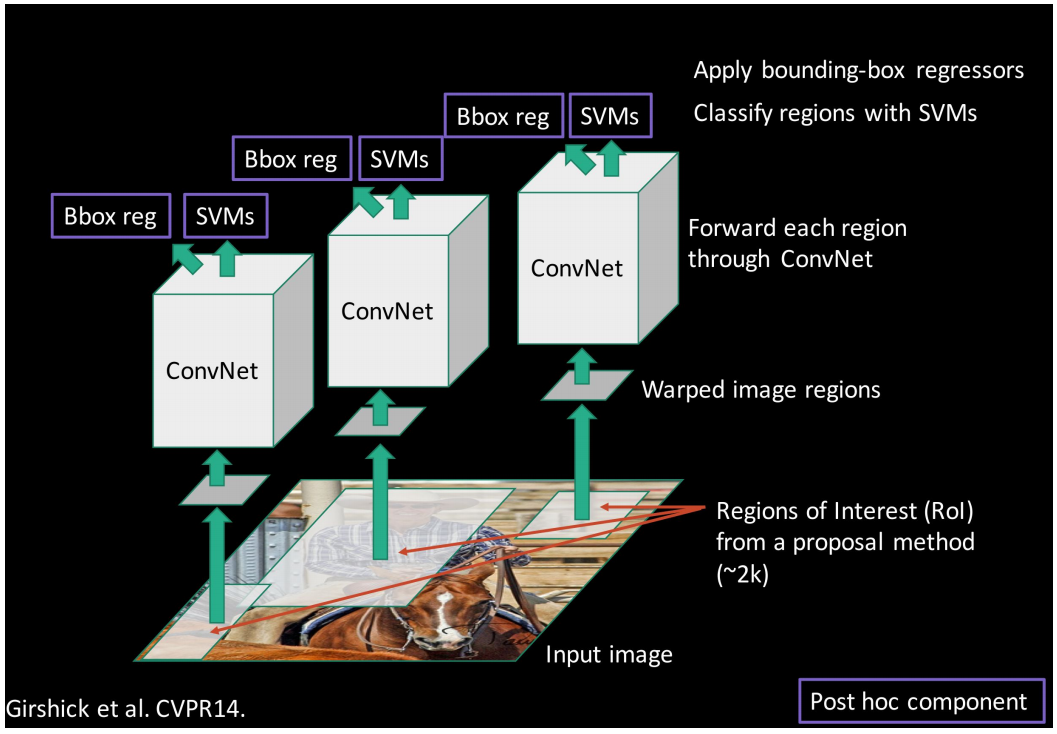
\includegraphics[width=0.85\linewidth]{R-CNN.png}
\centering
\captionsetup{justification=centering}
\caption{R-CNN \cite{girshick2014richrcnn} . Source: CS231-Stanford\protect\footnotemark}
\label{fig: R-CNN}
\end{figure}
\footnotetext{\label{fn:CS231-Stanford} Stanford:http://cs231n.stanford.edu/slides/2016/winter1516\_lecture8.pdf - Slide: 53 }


\begin{figure}[H]
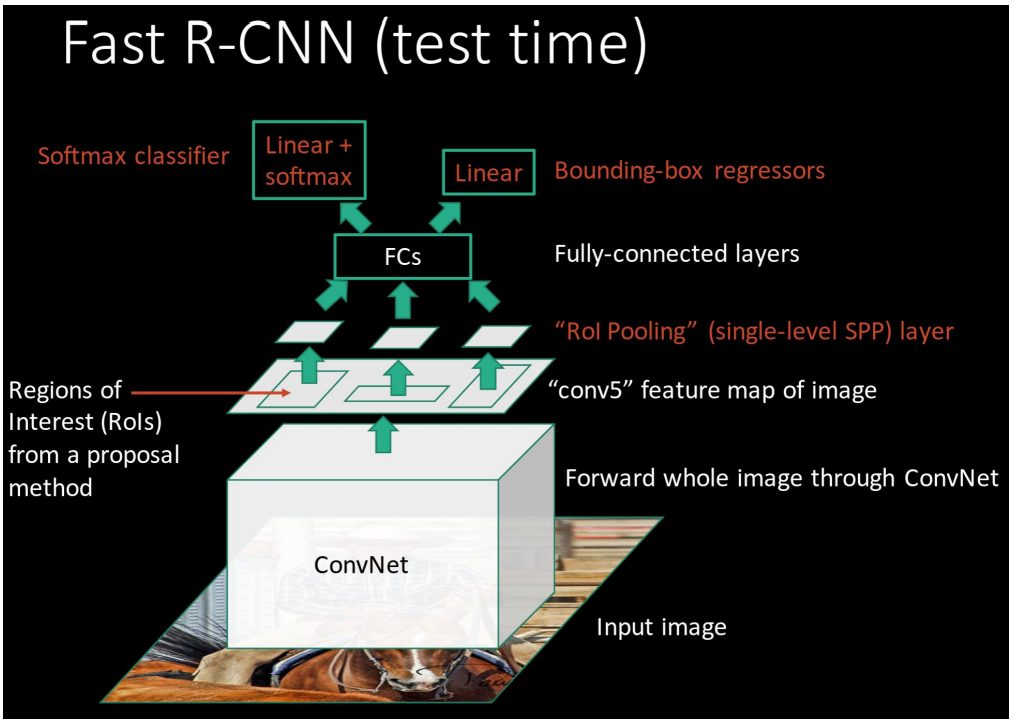
\includegraphics[width=0.85\linewidth]{Fast-RCNN.png}
\centering
\captionsetup{justification=centering}
\caption{Fast R-CNN \cite{girshick2015fast} . Source: CS231-Stanford\protect\footnotemark}
\label{fig: Fast R-CNN}
\end{figure}
\footnotetext{\label{fn:CS231-Stanford-1} Stanford:http://cs231n.stanford.edu/slides/2016/winter1516\_lecture8.pdf - Slide: 67 }

As the name suggests, Faster R-CNN is much faster than Fast R-CNN (see table \ref{fig: Compare-Dection-Time-Result-fasterrcnn}) w.r.t. test speed and accuracy. The big difference between Faster R-CNN (figure \ref{fig: Faster R-CNN} ) and Fast R-CNN (figure \ref{fig: Fast R-CNN})  is \textit{Region Proposal Network} (RPN). In case of  Fast R-CNN, RPN is external like Selective Search so it has to be trained explicitly. But in case of Faster R-CNN, RPN is a CNN network which is a part of whole object detector model (see figure \ref{fig: Faster R-CNN}).   

\begin{figure}[H]
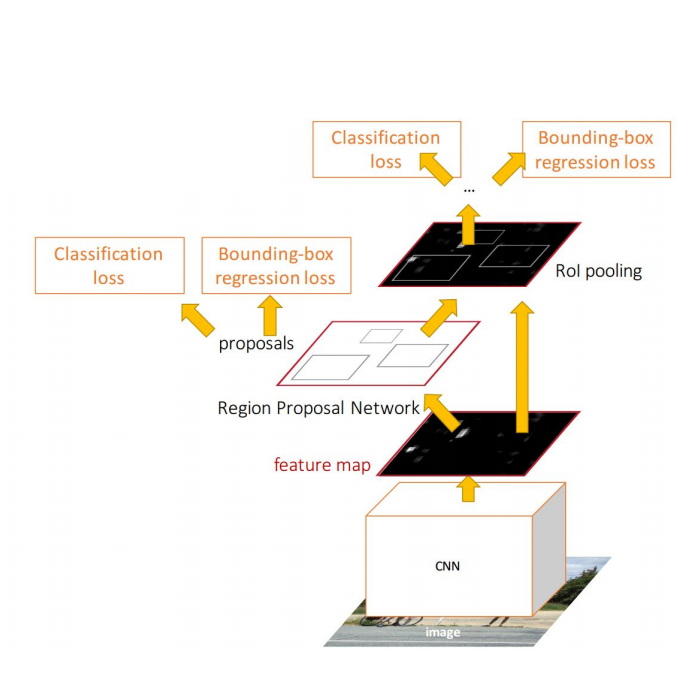
\includegraphics[width=0.85\linewidth]{Faster-RCNN.png}
\centering
\captionsetup{justification=centering}
\caption{Faster R-CNN. Source: \cite{ren2015faster}}
\label{fig: Faster R-CNN}
\end{figure}

Faster R-CNN has RPN. Classification and localization are using CNN and full connected neural network. So while training Faster R-CNN, there are four loss functions that have to be minimized. Four loss functions are  as follows (see figure \ref{fig: Faster R-CNN}):
\begin{itemize}
  \item RPN classification (anchor good / bad)
  \item RPN regression (anchor 	$\rightarrow$ proposal)
  \item Fast R-CNN classification (over classes)
  \item Fast R-CNN regression (proposal $\rightarrow$ box)
\end{itemize}

\textit{Anchors} helps in finding objects at different scale level \cite{ren2015faster} . So, the four losses are calculated at two levels, the first two at RPN level and the other two at output layer. Training Faster R-CNN is not easy like other CNN networks. It has a four stage training  \cite{ren2015faster} pipeline. In stage 1, RPN is trained then in stage 2 using the trained weights of RPN, "classifier and regression" network is trained. In stage 3, again RPN is trained but with full network, i.e. using the stage 2 weights of "classifier and regression" and in last stage "classifier and regression" are trained using the weights of the stage 3. Training is like an alternating fashion.


\begin{figure}[H]
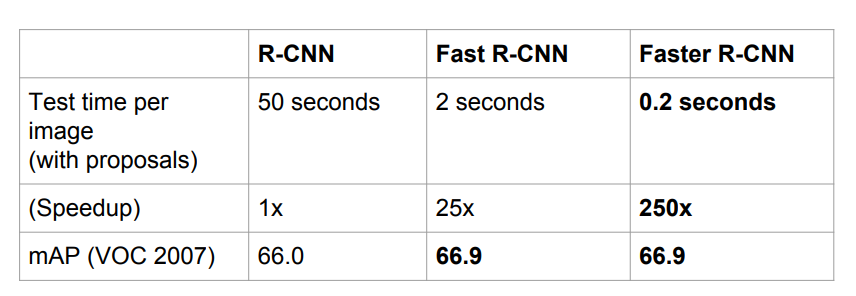
\includegraphics[width=0.85\linewidth]{campare-result-faster-rcnn.png}
\centering
\captionsetup{justification=centering}
\caption{Comparison between R-CNN, Fast R-CNN and Faster R-CNN on testing time and accuracy VOC-2007 \cite{ren2015faster} . Source: CS231-Stanford\protect\footnotemark}
\label{fig: Compare-Dection-Time-Result-fasterrcnn}
\end{figure}
\footnotetext{\label{fn:CS231-Stanford-2} Stanford:http://cs231n.stanford.edu/slides/2016/winter1516\_lecture8.pdf - Slide: 84 }


\section{Experiment}

In the previous experiments, the simulated datasets were used i.e. using the 3d structure of Ribosomes taken from the \textit{EM Databank} \footnote{\label{fn:emdatabank}EM-Databank: http://www.emdatabank.org/} many projections were created and using these projections micrographs were generated. But to get the correct accuracy of models, it has to be tested against \textit{Real Micrographs} of Ribosomes or Viruses. 

\textit{Real Micrographs} comes with many challenges with respect to \textit{Particle Picking}. The first and the biggest challenge is marking of the particles on the micrograph. As the models are semi-automated, so to train classifiers there is a need of $\sim$6K marked particles on micrograph. Manual marking takes time and more importantly one's need to be Biologist as identifying between heterogeneous projections and ice is hard. So for the experimental purpose and to save time, datasets taken for experiments are having markings and these marking are done by the trusted third-party. The second challenge is the size of datasets. Size of dataset varies from  500 GB to few TB (say 2 TB, our observation) in which dataset has movie files and each files may size up to 8 GB. So handling these files requires bigger size RAM and optimized algorithm.
\subsection{Dataset}
This section will talk about 4 dataset used in experiments. The dataset required for experiment need to have markings of particles in the micrograph. Otherwise these markings have to be done manually by Biologist or if someone else is doing then markings have to be verified by Biologist because wrongly marked particle may lead to poor classifier. Out of 4 datatset, three datasets are taken from \textit{EM Databank} \footnote{\label{fn:emdatabankchalange}EM-Databank: http://challenges.emdataresource.org/?q=2015\textunderscore map\textunderscore challenge} with particles marked via \textit{RELION} tool and remaining one dataset taken from the \textit{IISER - Trivandrum} with marking done by \textit{Dr. Ramanathan Natesh}\footnote{Dr. Ramanathan Natesh: http://faculty.iisertvm.ac.in/natesh/}. Below is the detailed description about the datasets.

\subsubsection{Dataset-1: T20S-Proteasome (T20)}\label{subsec:T20S-Proteasome}
This dataset is taken from the EM-Databank having EMD id as \textbf{EMD-6287} and EMPAIR id as \textbf{EMPIAR-10025}\footnote{\label{fn:EMPIAR-10025-3}EMPIAR-10025:http://www.ebi.ac.uk/pdbe/emdb/empiar/entry/10025/}. The 3D structure of T20-Proteasome is shown in figure \ref{fig:EMPIAR-10025-3d-struct}. This 3D structure will help in finding error in 3D reconstruction. 

\begin{figure}[H]
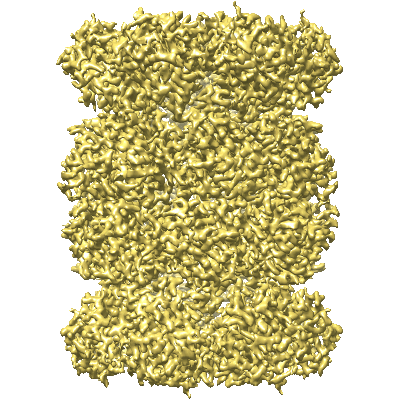
\includegraphics[width=0.45\textwidth]{EMPIAR-10025}
\centering
\captionsetup{justification=centering}
\caption{T20S Proteasome\protect\footnotemark 2.8 Angstrom resolution}
\label{fig:EMPIAR-10025-3d-struct}
\end{figure}
\footnotetext{\label{fn:empair-10025databank}EBI data bank: http://www.ebi.ac.uk/pdbe/emdb/empiar/entry/10025/}

Total dataset size is 369 GB, which contains movie files each of size 3 GB in \textbf{mrc} format (mrc is the globally known standard format for saving raw images take from EM) Each having 38 frames per movie files. Dimension of each frame is 7420x7676. Markings of particles are done via a RELION \cite{scheres2012relion} software but problem is that this RELION gives lot many other information, so these marking has to be parsed before it can be used. But, one issue with dataset is that not all particles are marked i.e. each micrograph has around 1500 particles or more but markings are only for approximately 250 particles.

\begin{figure}[H]
\centering
\begin{subfigure}{.5\textwidth}
\centering
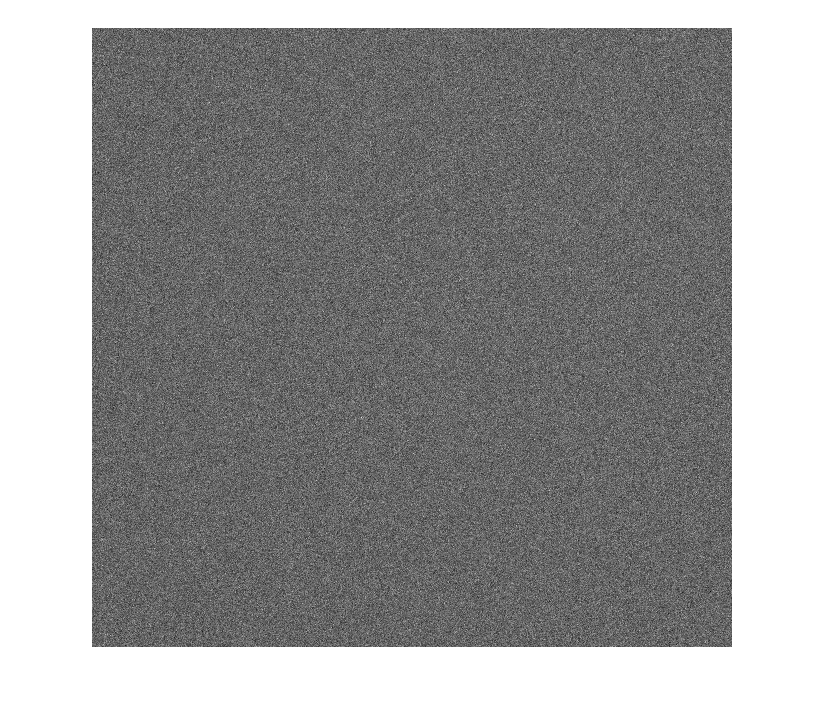
\includegraphics[width=0.5\linewidth]{EM-10025-micrograph-full_micrograph}
\captionsetup{justification=centering}
\caption{ Full Scale }
\end{subfigure} 
\begin{subfigure}{.48\textwidth}
\centering
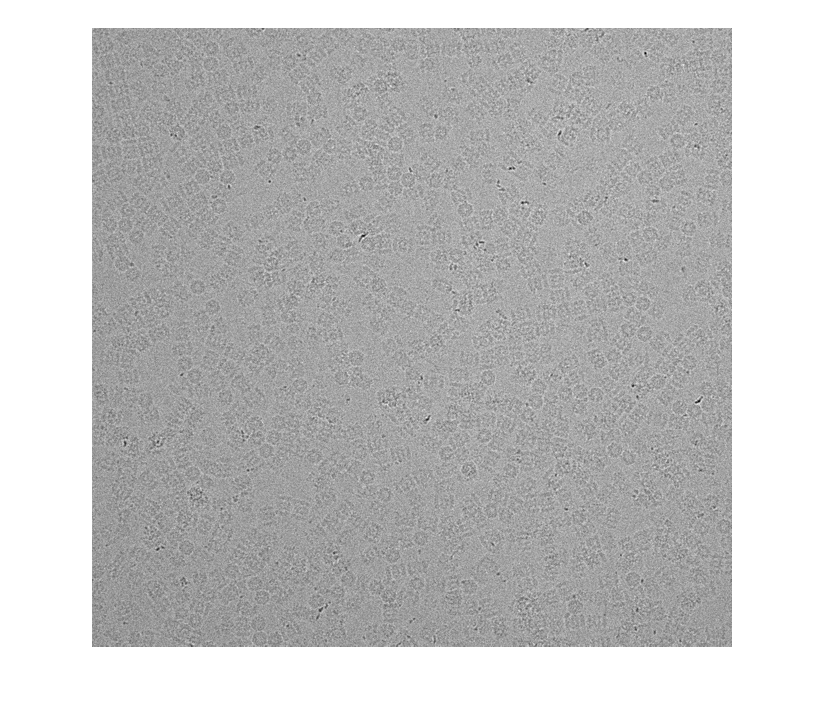
\includegraphics[width=0.5\linewidth]{EM-10025-micrograph-full-down-12_micrograph}
\captionsetup{justification=centering}
\caption{Downsampled by 12}
\end{subfigure}
\captionsetup{justification=centering}
\caption{T20S Proteasome Averaged Micrograph, In Full Scale view, it is very hard to visualize where are the particles. But after reasonable downsampling particles can  visualized }
\label{fig:EM-10025-Avg-micrograph}
\end{figure}

\subsubsection{Dataset-2: 80S-Ribosome (80S)}\label{subsec:80S-Ribosome}
80S-Ribosome is the dataset from the EM-Databank having EMD id as \textbf{EMD-2660} and EMPAIR id as \textbf{EMPIAR-10028}\footnote{\label{fn:EMPIAR-10025-1} EMPIAR-10025:http://www.ebi.ac.uk/pdbe/emdb/empiar/entry/10028/}. Single particle 3d reconstruction have 3.2 angstroms resolution see the figure \ref{fig:EMPIAR-10028-3d-struct}.

\begin{figure}[h]
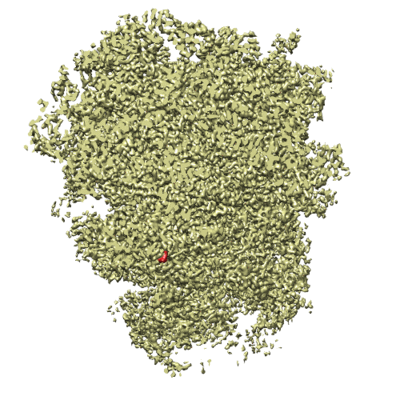
\includegraphics[width=0.45\textwidth]{EMPIAR-10028}
\centering
\captionsetup{justification=centering}
\caption{80S Ribosome\protect\footnotemark 3.2 Angstrom resolution}
\label{fig:EMPIAR-10028-3d-struct}
\end{figure}
\footnotetext{\label{fn:empair-10028databank}EBI data bank: http://www.ebi.ac.uk/pdbe/emdb/empiar/entry/10028/}

Initial dataset of 80S-Ribosome from the databank is very large, it is approximately equal to the 2 TB (Terabytes). This dataset contains lots of meta data related to each file which will not be used in particle picking but might be used at the time of reconstruction. Each file is a movie file of size 3 GB and having dimension of 4096x4096. Per movie file has 47 frames. Multiple frames will help in removing the noise by averaging of these frames. Figure \ref{fig:EM-10028-Avg-micrograph} shows the averaged micrograph (average of 47 frames) of a movie file. Marking of particle is done using the RELION and each micrograph has approximately 50 to 60 particles.

\begin{figure}[h]
\centering
\begin{subfigure}{.5\linewidth}
\centering
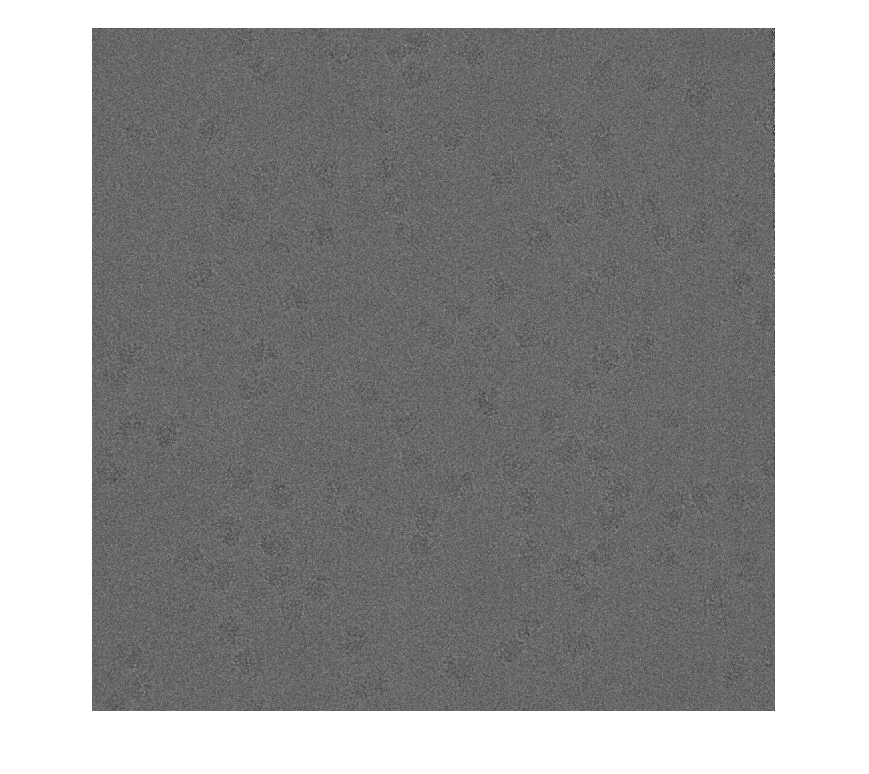
\includegraphics[width=0.5\linewidth]{EM-10028-micrograph-full_micrograph}
\captionsetup{justification=centering}
\caption{ Full scale }
\end{subfigure} 
\begin{subfigure}{.48\linewidth}
\centering
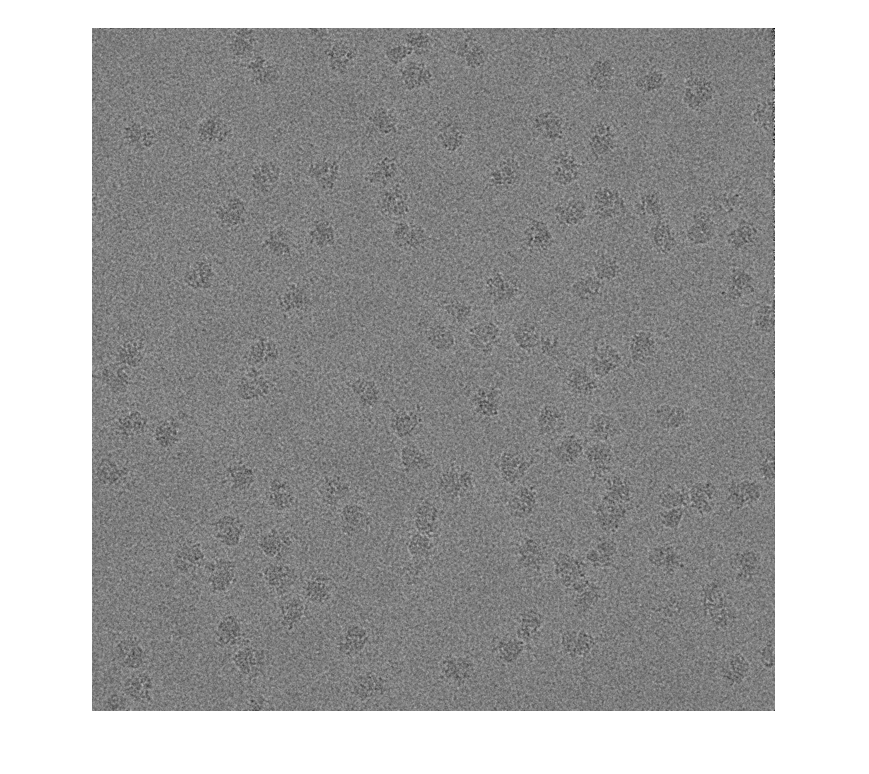
\includegraphics[width=0.5\linewidth]{EM-10028-micrograph-full-down-6_micrograph}
\captionsetup{justification=centering}
\caption{Downsampled by 6}
\end{subfigure}
\captionsetup{justification=centering}
\caption{80S Ribosome Averaged Micrograph. In Full Scale view, it is very hard to visualize where are the particles. But after reasonable downsampling particles can  visualized}
\label{fig:EM-10028-Avg-micrograph}
\end{figure}


\subsubsection{Dataset-3: $\beta$-Galactosidase ($\beta$-G)}\label{subsec:B-Galactosidas}

$\beta$-Galactosidase is a dataset from the EM-Databank having EMD id as \textbf{EMD-5995} and EMPAIR id as \textbf{EMPIAR-10012/1003}\footnote{\label{fn:EMPIAR-10025-2}EMPIAR-10025:http://www.ebi.ac.uk/pdbe/emdb/empiar/entry/10013/}. Single particle 3D reconstruction at 3.2 angstroms resolution can be seen in figure \ref{fig:EMPIAR-10012-3d-struct}.

\begin{figure}[h]
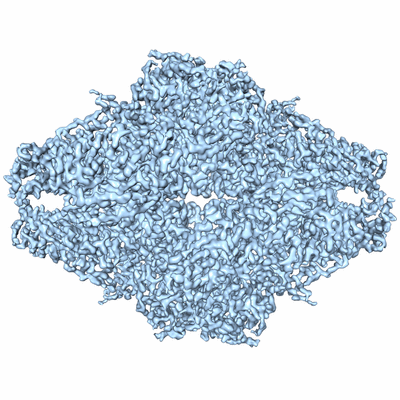
\includegraphics[width=0.45\textwidth]{EMPIAR-10012}
\centering
\captionsetup{justification=centering}
\caption{ $\beta$-Galactosidase\protect\footnotemark 3.2 Angstrom resolution}
\label{fig:EMPIAR-10012-3d-struct}
\end{figure}
\footnotetext{\label{fn:empair-10012databank}EBI data bank: http://www.ebi.ac.uk/pdbe/emdb/empiar/entry/10013/}

Dataset is taken from the EM-databank which is approximately equal to the 108 GB. Each file is a averaged file of size 256 MB and has dimension of 7420x7676 Figure \ref{fig:EM-10028-Avg-micrograph} shows the micrograph. Marking of particle is done using the RELION and each micrograph has thousands of particles but out of which approximately 50 are marked.

\begin{figure}[h]
\centering
\begin{subfigure}{.5\textwidth}
\centering
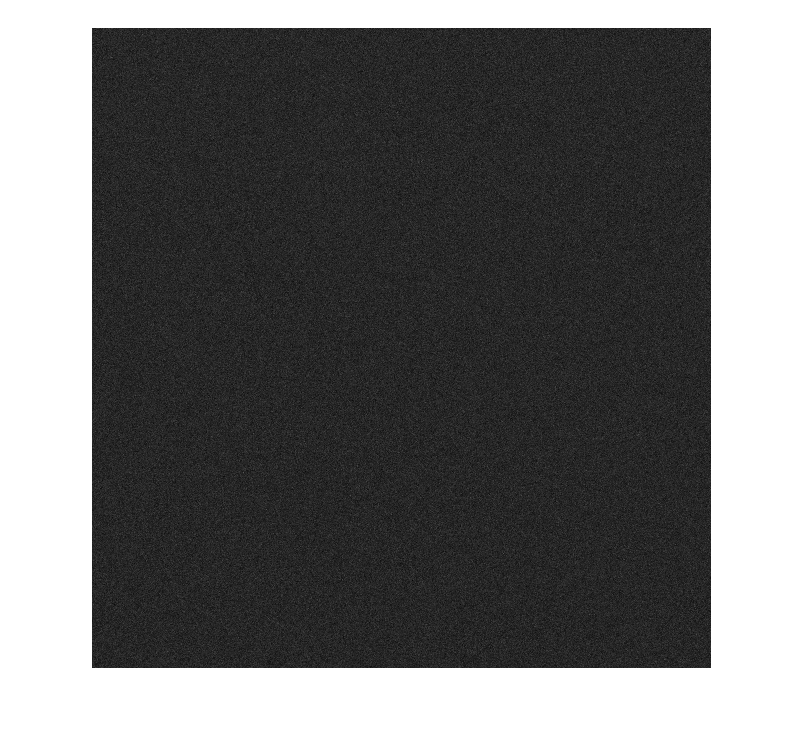
\includegraphics[width=0.5\linewidth]{EM-10012-micrograph-full_micrograph}
\captionsetup{justification=centering}
\caption{ Full Scale }
\end{subfigure} 
\begin{subfigure}{.48\textwidth}
\centering
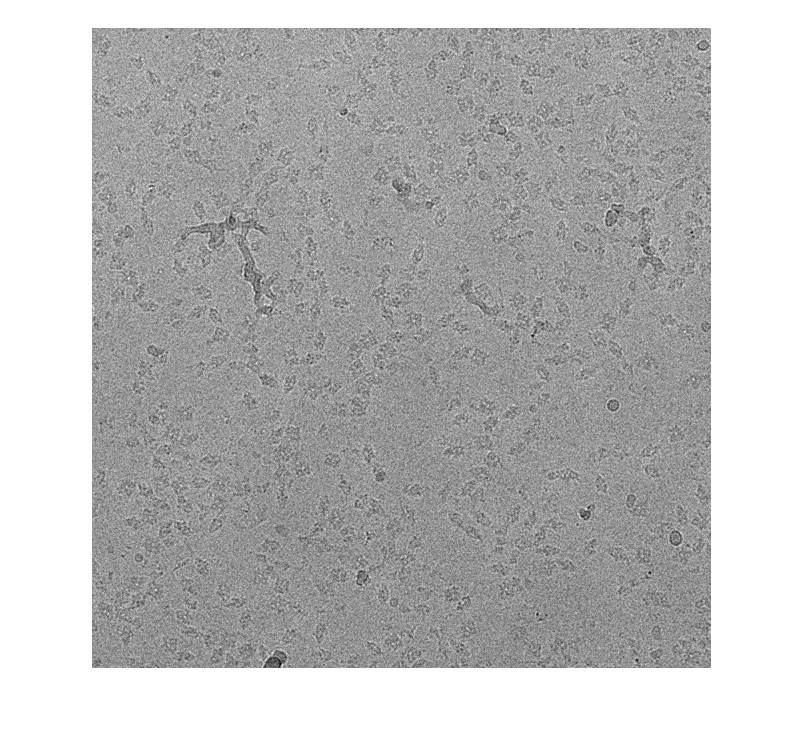
\includegraphics[width=0.5\linewidth]{EM-10012-micrograph-full-down-12_micrograph}
\captionsetup{justification=centering}
\caption{Downsampled by 12}
\end{subfigure}
\captionsetup{justification=centering}
\caption{ $\beta$-Galactosidase Averaged Micrograph. In Full Scale view, it is very hard to visualize the particles. But after reasonable downsampling particles can  visualized}
\label{fig:EM-10012-Avg-micrograph}
\end{figure}


The table \ref{tbl:Dataset} shows the detail about dataset in brief
\begin{table}[H]
\centering
  \begin{tabular}{|c|c|c|c|c|} 
    \hline \hline
      Dataset & Size(GB) & Type & Number of files & Dimension  \\ [0.5ex] 
    \hline \hline
    T20S Proteasome & 369 & Movie & 196 & 7420x7670 \\\hline
    80S Ribosome & 2048 & Movie & 1081 & 4096x4096 \\\hline
    $\beta$-Galactosidase & 108 & Averaged & 509 & 7420x7670 \\\hline
    \hline 
  \end{tabular}
\caption{Dataset}
\label{tbl:Dataset}
\end{table}

\subsection{Dataset Pre-Processing}
There are many implementation challenges when these datasets are considered. As these datasets are extremely large in terms of "size of each file" so, handling these becomes tough. Below are the challenges:

\subsubsection{File Extension}
First thing in pre-processing is the file extension. Files are having  \textbf{mrc} extensions. MRC stands for \textit{Medical Research Council}. As mrc extension is not the standard format for an image or the movie. So, there is a need of parser for reading mrc extension. In mrc, each file is divided into two parts, first is the header section and next is data section. Header describes how data is presented in data section and meta data, for example NX and NY field specify the number of columns and rows in 3D data array respectively. For more information related to header, see header table \ref{fig:mrc-header}. As it is not a daily used format, so you may need to write your own parser depending upon the language.

\begin{figure}[h]
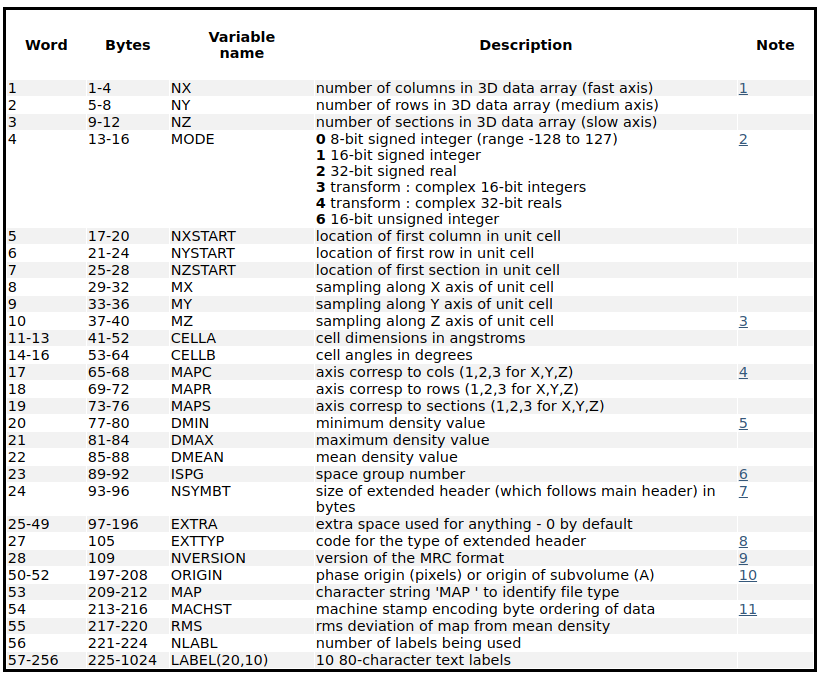
\includegraphics[width=0.75\textwidth]{mrc_header.png}
\centering
\captionsetup{justification=centering}
\caption{MRC header\protect\footnotemark format}
\label{fig:mrc-header}
\end{figure}
\footnotetext{\label{fn:mrc-header}MRC header: http://www.ccpem.ac.uk/mrc\textunderscore format/mrc2014$.$php}

\subsubsection{Handling Movie File}
The second part in pre-processing is to convert the movie file into the average file. Averaging is done by adding up all the frames of movie file and then dividing each pixel by the number of the frames. But there is a problem, which is the size of each movie file. As each file size might go up to 8 to 9 GB for different types of datasets, so reading all the frames and then finding average will require a lot of main memory (RAM). In our case, maximum size of file for 80S-Ribosome is 3 GB (see section \ref{subsec:80S-Ribosome}). So, to handle this problem, write mrc file parser such that it gives one frame at a time. By this, find average simultaneously while reading the movie file.  Averaging will help in reducing the noise level which will further improve the classifier.


\subsubsection{Parsing Particles Marking}
The next setup in pre-processing is to parse the particle marking because each datasets has different style of representation for storing the marking. Like in case of T20S-Proteasome (\ref{subsec:T20S-Proteasome}), marking is done by RELION and for all the micrographs markings are saved in a single file with lots of other meta data and header for the meta data. In case of 80S-Ribosome (\ref{subsec:80S-Ribosome}), marking is done through RELION and each micrograph has it's own marking file containing x and y location with meta data. For $\beta$-Galactosidase (\ref{subsec:B-Galactosidas}), each micrograph has its own marking file but marking file contains the bounding box (eman-box) information rather than coordinates of particles. Images \ref{fig:Particle-Marking-Dataset} shows the snippet for these three molecules projections marking.

\begin{figure}[h]
\centering
\begin{subfigure}{.5\textwidth}
\centering
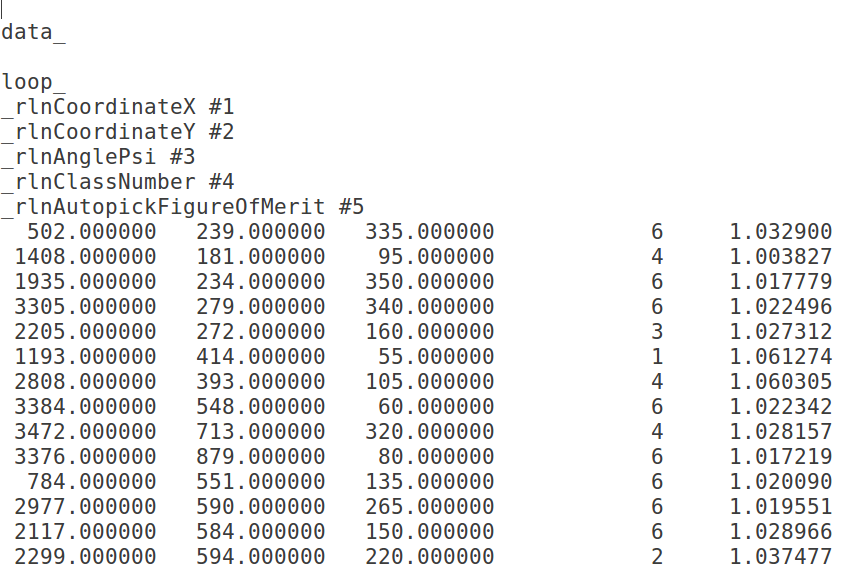
\includegraphics[width=0.5\linewidth]{marking-EM-10028.png}
\captionsetup{justification=centering}
\caption{ 80S-Ribosome }
\end{subfigure} 
\begin{subfigure}{.48\textwidth}
\centering
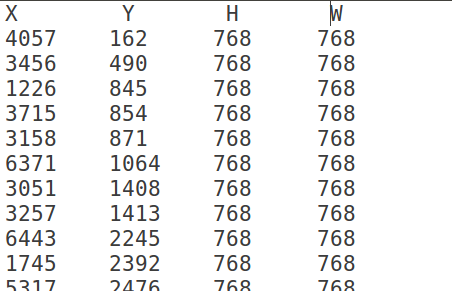
\includegraphics[width=0.5\linewidth]{marking-EM-10012.png}
\captionsetup{justification=centering}
\caption{$\beta$-Galactosidase}
\end{subfigure}
\begin{subfigure}{.8\textwidth}
\centering
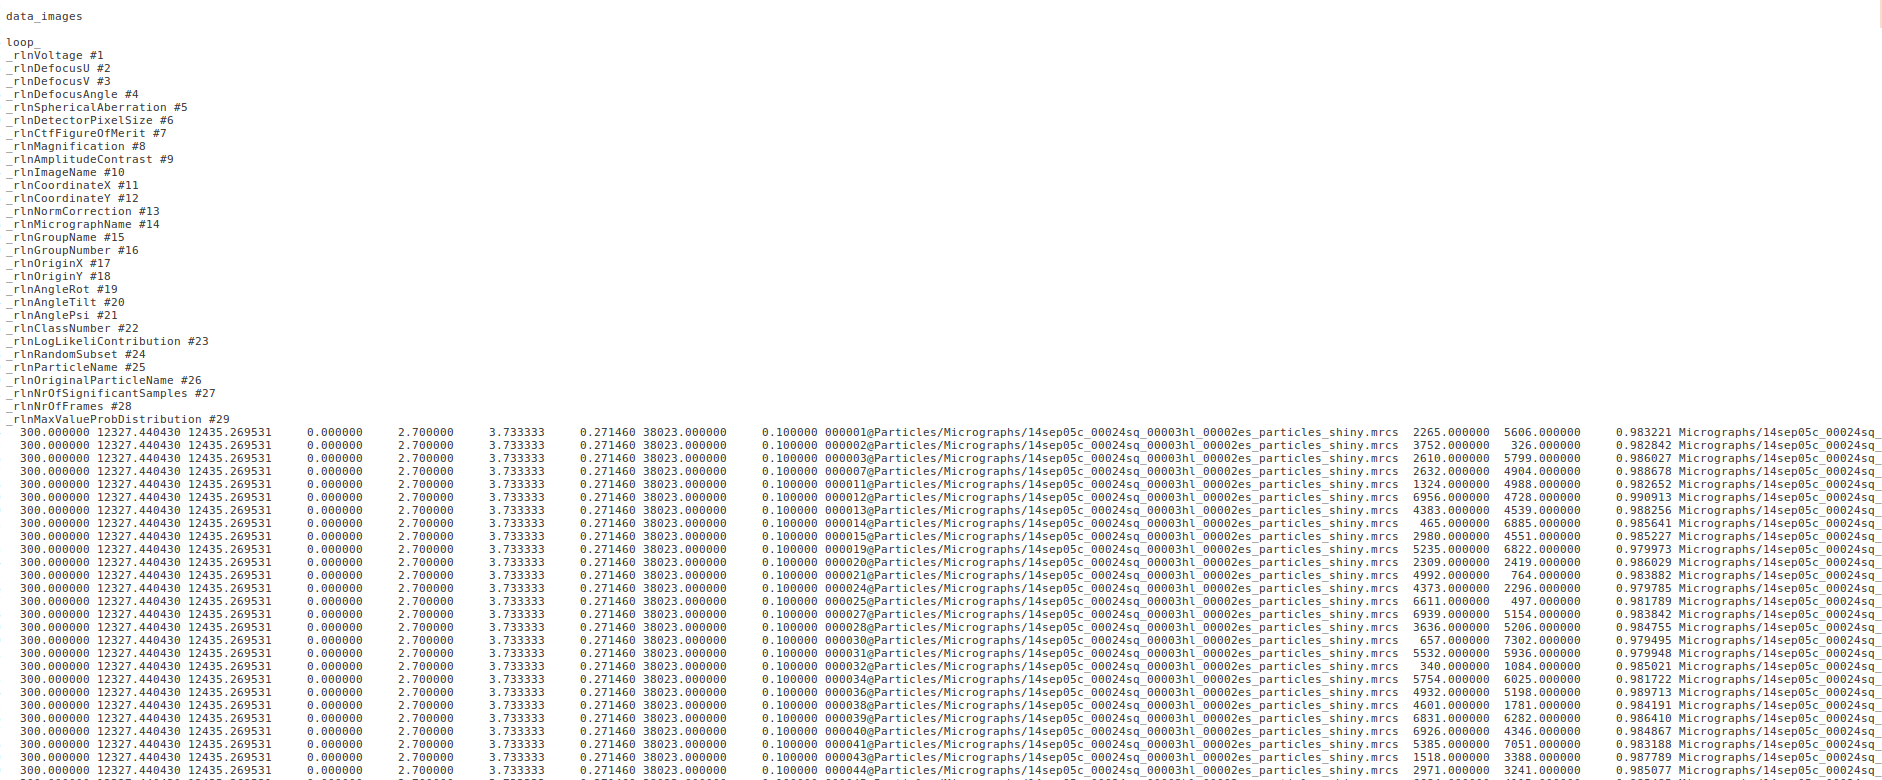
\includegraphics[width=0.8\linewidth]{marking-EM-10025.png}
\captionsetup{justification=centering}
\caption{T20S-Proteasome}
\end{subfigure}
\captionsetup{justification=centering}
\caption{ Particle Marking Data Format. All the three datasets have different representation format. So, developing generic parser is not possible.}
\label{fig:Particle-Marking-Dataset}
\end{figure}

Training SVM and Random Forest requires train dataset and for validating the classifier, test dataset is needed. As the correct dataset is in mrc format so these cannot be directly given to model for training and on above that these are micrographs. First thing is to convert mrc micrograph to jpeg/png or directly use the image for further pre-processing. In the experiments raw micrographs are being used. Then, for generating the train and test dataset, crop the projections from micrograph by using the marking of the particles of their respective dataset. This will give \textit{positive class} sample (see images \ref{fig:Positive-Projection}) but for training classifier \textit{negative class} samples such as background, ice particles, partially covered particle, multiple particles and different types of other particles are also required. \\
\subsubsection{Generating Train and Test Set - SVM and Random Forest}

\begin{figure}[h]
\centering
\begin{subfigure}{.5\textwidth}
\centering
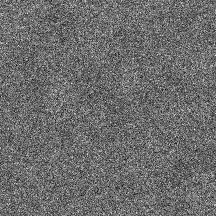
\includegraphics[width=0.5\linewidth]{pos-EM-10025.png}
\captionsetup{justification=centering}
\caption{ T20S-Proteasome }
\end{subfigure} 
\begin{subfigure}{.48\textwidth}
\centering
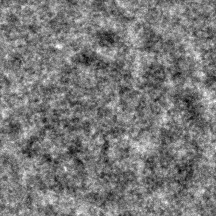
\includegraphics[width=0.5\linewidth]{pos-EM-10028.png}
\captionsetup{justification=centering}
\caption{ 80S-Ribosome }
\end{subfigure}
\begin{subfigure}{.5\textwidth}
\centering
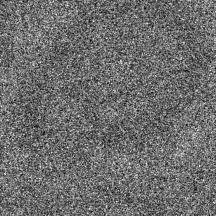
\includegraphics[width=0.5\linewidth]{pos-EM-10012.png}
\captionsetup{justification=centering}
\caption{$\beta$-Galactosidase }
\end{subfigure}
\captionsetup{justification=centering}
\caption{ Positive Projection after cropping (Dimension 216x216)}
\label{fig:Positive-Projection}
\end{figure}

Negative samples (see images \ref{fig:Negative-Projection}) plays a very vital role during classification  of particle and non-particle. In the experiment, for generating negative samples \cite{chen2012detection}, marking of positive particles were used. Given $(x,y)$ location of a particle on the micrograph and maximum dimension of particle  which will be known in prior (in our case it is 216x216) then two negative sample are generated by cropping at location $(x+ max\_size/2, y + max\_size/2)$ and $(x- max\_size/2, y - max\_size/2)$. This will handle the case of partial particle, background and multiple particles. In our case, adding different other types of particles in negative set are not required because this trained model will only be used on image having only one type of particle. 

\begin{figure}[h]
\centering
\begin{subfigure}{.5\textwidth}
\centering
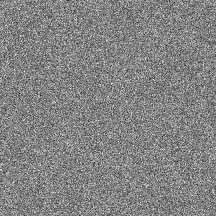
\includegraphics[width=0.5\linewidth]{neg-EM-10025.png}
\captionsetup{justification=centering}
\caption{ T20S-Proteasome }
\end{subfigure} 
\begin{subfigure}{.48\textwidth}
\centering
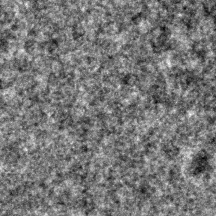
\includegraphics[width=0.5\linewidth]{neg-EM-10028.png}
\captionsetup{justification=centering}
\caption{ 80S-Ribosome }
\end{subfigure}
\begin{subfigure}{.5\textwidth}
\centering
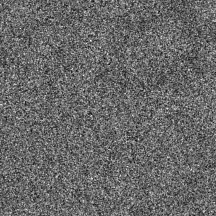
\includegraphics[width=0.5\linewidth]{neg-EM-10012.png}
\captionsetup{justification=centering}
\caption{$\beta$-Galactosidase }
\end{subfigure}
\caption{Negative Sample (Dimension 216x216)}
\label{fig:Negative-Projection}
\end{figure}

\subsubsection{Generating Train and Test Set - Faster R-CNN}\label{subsec:gen-train-test-faster-rcnn}
Faster R-CNN is the variant of Convolution Neural Network (CNN). But unlike traditional CNN, it does both classification and object detection in given input image. For training  Faster R-CNN, it requires images with bounding box (top-left x,top-left y,height, width) information related to the interested object rather single-single positive and negative image (216x216).\\

In dataset, single micrograph dimension is very large and total count of these micrographs (approx. 7000x7000) are also very less. So whole dataset of micrographs are divided into train and test set. Then, each micrograph is further divided into 1000x1000 sub-micrographs. For each sub-micrograph, bounding box related to the objects present in it is also required. So these bounding boxes are calculated by finding particles coordinates which are marked and which lies in that sub-micrograph. This whole thing is also done for test set and while testing rather than passing whole big micrograph sub-micrographs (1000x1000) are passed. Image \ref{fig:fastercnn-EM110025-train} shows the one of 1000x1000 cropped micrograph from the big micrograph and true marking of particles in the bounding box format.\\

Faster R-CNN also needs negative sample as that of SVM and Random Forest. But in this case there is no need of generating separate negative samples. The Faster R-CNN network will treat shifted bounding box from it's original position as the negative sample. This is very much similar to the way of generating negative sample in the case of SVM and Random Forest.

\begin{figure}[h]
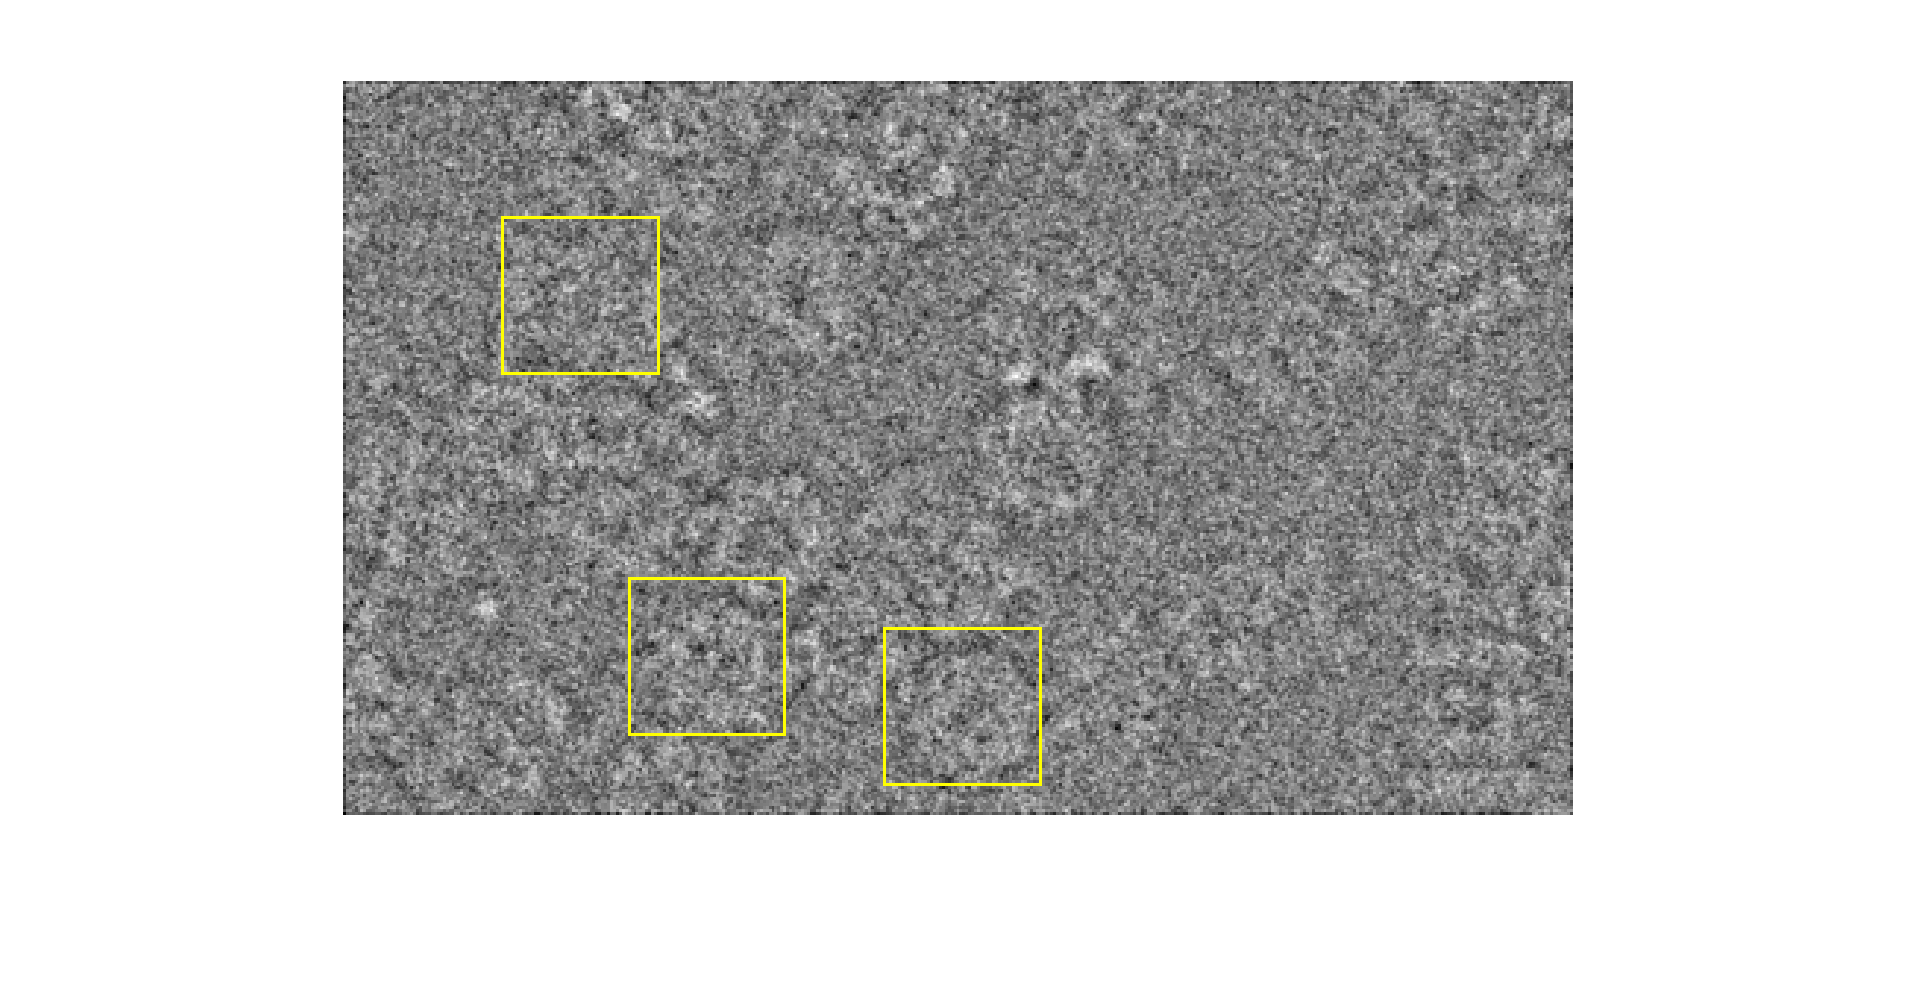
\includegraphics[width=0.95\textwidth]{fastercnn-EM110025.png}
\centering
\captionsetup{justification=centering}
\caption{1000x1000 cropped micrograph of T20S-Proteasome with bounding box}
\label{fig:fastercnn-EM110025-train}
\end{figure}


\subsection{Train and Test Model Architecture}
As seen in section \ref{sec:train_arch} and \ref{sec:detector_ach} about the multi scale architecture. Scale of the model is the tuning parameter. Observation from the previous experiments is that if n-1 scale are dropped in n downscale model then accuracy of the model will not be affected much, say  for 3-downscale model $[8,4,2]$. If model is created only for downscale rate 8 then, it will give approximately same result as that of combined 3-downscale $[8,4,2]$. Reason for this effect is that classifier trained on higher resolution images gives poor result as compared to lower resolution image because in our application dataset size was very small. So in case of lower resolution image say "downscale model-8", less amount of data will required for training but in case of higher resolution image say "downscale model-4" , large amount of data will be required  as compared to "downscale model-8 to get same amount of accuracy.


\subsection{Feature Extraction}
As train image dimensions are very large i.e. for 216x216 image will have 46656 pixels which is a huge number if features are considered. So to train classifier like SVM, Random forest or any other (apart from deep nets) there is a need of few feature points i.e. in few hundreds or thousands otherwise training on raw image will take many hours and resources
\cite{chen2012detection}. \\

In the experiment, PCA (Principal Component Analysis) was used for reducing the dimension of the train and test set. Number of principle components taken were 1000, so the dimension of image was reduced from 46656 to 1000 pixels. These PCA coefficients of images were then used for training the classifier. For testing test image (say 216x216), first PCA coefficients was computed or one can say that test image was projected on to the PCA space and then it was given to detector for prediction. Because classifier is trained in PCA space, so testing has to be done in PCA space. Testing on micrograph follows (\ref{sec:detector_ach}) architecture, otherwise if overlapping patches are cropped on original micrograph then it will take many hours.

\begin{table}[h]
\centering
\begin{tabularx}{\textwidth}{|*{8}{Y|}}
\hline\hline
\multirow{2}{*}{Dataset} & \multicolumn{3}{c|}{Train set} & \multicolumn{3}{c|}{Validation set} & \multirow{2}{*}{\shortstack{Test set \\ (mg*)}}\\
\cline{2-7}
             & $+$ve & -ve & Total & $+$ve & -ve & Total & \\
\hline
T20S & 6,000 & 12,000 & 18,000 & 2,072 & 8,288 & 10,360 & 40  \\ \hline
80S  & 6,000 & 12,000 & 18,000 & 4,739  & 12,030 & 16,769 & 80 \\ \hline
$\beta$-G & 6,000 & 12,000 & 18,000 & 3,395 & 13,578 & 16,973 & 40 \\ \hline
\hline
\end{tabularx}
\captionsetup{justification=centering}
\caption{Train and Test Dataset for SVM and Random forest (mg* stands for Micrograph)}
\label{tbl:Train-test-svm-rf-Dataset}
\end{table}


\subsection{Classifier - Support vector machine}
For particle detector (\ref{sec:detector_ach}), a classifier is needed. One type of classifier is \textit{Support vector machine} (SVM). In our experiments, SVM was used as one type of the classifier. For training the SVM, dataset was divided into train and test set. Division of the dataset is mentioned in the table \ref{tbl:Train-test-svm-rf-Dataset}.  For training SVM, kernel used are linear, Radial Basis Function (RBF) and polynomial of degree 2 \& 3. But accuracy given by linear kernel is much better than RBF and polynomial 2 \& 3 kernel. Also, detector model used was downscale-model-12 for all the datasets, which means each image was first downsampled by 12 and then SVM was trained using the downsampled image.

\subsubsection{Result}
For training SVM with 18K images, training took couple of hours but the detection on full micrograph of dimension \~7000x7000 took 25-30 mins. Results for SVM with linear kernel are shown in table \ref{tbl:SVM-result}. Precision is very low as compared to the accuracy of the model but this is because for T20S-Proteasome,  marking of particles per micrograph is very low i.e. micrograph contains thousands of particles but only few hundreds are marked.

\begin{table}[H]
\centering
  \begin{tabularx}{\textwidth}{|*{7}{Y|}}
    \hline\hline
    \multirow{2}{*}{Dataset} &\multirow{2}{*}{Recall} & \multirow{2}{*}{Precision} &\multicolumn{4}{c|}{Translation error (pixel)}\\
    \cline{4-7}
             & & & min. & max. & avg. & median \\
    \hline
T20S & 96\% & 16.96\% & 0 & 108 & 39 & 39 \\ \hline
80S  & 96.6\% & 66.91\% & 0 & 108  & 25 & 22 \\ \hline
$\beta$-G & 94\% & 9.48\% & 0 & 105 & 24 & 20 \\ \hline
\hline
\end{tabularx}
\caption{SVM Result}
\label{tbl:SVM-result}
\end{table}

Table \ref{tbl:SVM-result} shows the average result for the test micrographs (see table \ref{tbl:Train-test-svm-rf-Dataset}). The translation is very important. More the translation error, higher will be the reconstruction error if algorithm is not robust to translation error. So, the table shows the minimum, average, maximum and median translation error. Figure \ref{fig: SVM-Translation_Error_Histogram} shows the translation error histogram for all the particles. 


\begin{figure}[H]
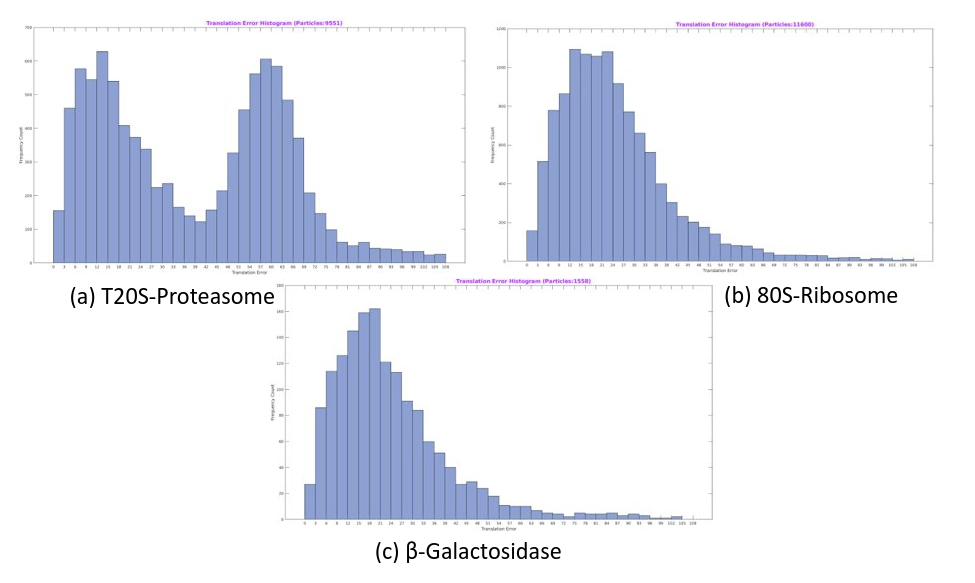
\includegraphics[width=1\linewidth]{svm-all-Translation_Error_Histogram.png}
\centering
\captionsetup{justification=centering}
\caption{SVM-Translation Error Histogram}
\label{fig: SVM-Translation_Error_Histogram}
\end{figure}

Micrographs \ref{fig: SVM-micrograph-marking} shows the particles marking on the test micrograph for all the datasets. Red mark is the predicted location by the SVM classifier and green is ground truth location. From the T20S-Proteasome and $\beta$-Galactosidase micrograph, one can observe that predicted particles (red marking) is much larger than (green marked) ground truth particles. Reason for this is that micrographs contains much more particles than the originally marked once and  our classifier has marked other particles for which ground truth locations are unknown. Because of this the precision of the model is very low. In case of 80S-Ribosome, dataset has marking for almost all the particles that's why its precision (table \ref{tbl:SVM-result}) is very good as compared to other dataset.

\begin{figure}[H]
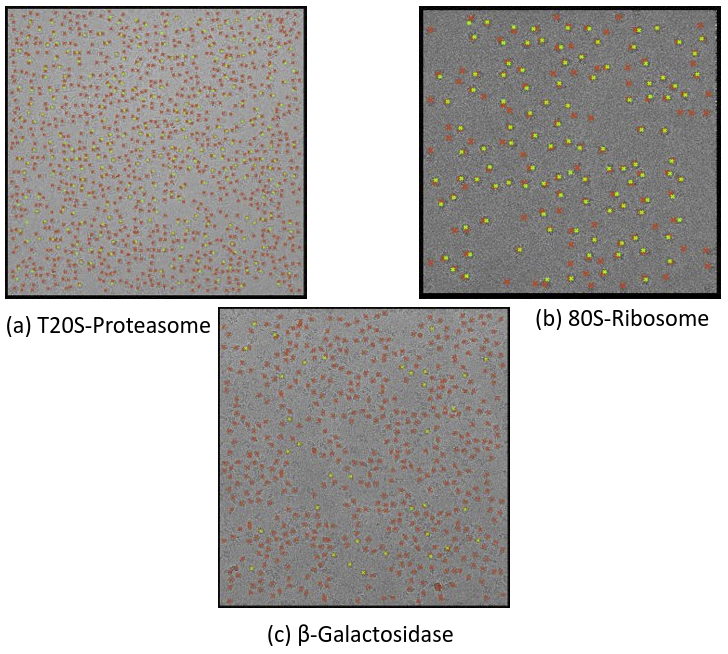
\includegraphics[width=0.98\linewidth,height=10cm]{svm-all-result.png}
\centering
\captionsetup{justification=centering}
\caption{SVM- Particle marking Results. Red: Predicted location. Green: Ground Truth}
\label{fig: SVM-micrograph-marking}
\end{figure}

\subsection{Classifier - Random Forest}
Random Forest classifier is trained on all the dataset with the same configuration. The size of train set is same for the three datasets which are T20S-Proteasome, 80S-Ribosome and $\beta$-Galactosidase (see table \ref{tbl:Train-test-svm-rf-Dataset}). Number of forest required for getting good accuracy in less amount of time are tuned. During tuning, it is found out that with 40 trees, the accuracy of classifier goes down and with 80 trees, detection time is large. Also if 50 trees are taken then accuracy of classifier was approximately same as of 80 trees and detection time is also less as compared to 80 trees. So, for all the dataset number of trees generated are 50.


\subsubsection{Result}
Time required to train Random Forest was approximately 15-20 mins whereas testing on whole micrograph took around couple of hours. The Reason for this is the  large number of patches from the micrograph. As the model is downscale-model-12, so micrograph of size 7420x7670 after downsampling by 12 will become 619x640. This test micrograph is given to the detector. Detector will then take out patches of dimension 18x18 (max size of particle is 216x216 and downsampled by 12 will give 18x18) with stride as 1, which will come out to 373822 patches. There are 50 trees and to test for each patch if it takes 2 sec (CPU based Random Forest) then total time comes out be be 8 hrs $(373822 *2 /(60*60*24))$. But, as our detector used multiple CPU for detection so with 10 core CPU overall time comes out to be 2.5-3 hrs including the meta data processing such as finding PCA of those patches before giving it to the Random Forest classifier.

\begin{table}[H]
\centering
  \begin{tabularx}{\textwidth}{|*{7}{Y|}}
    \hline\hline
    \multirow{2}{*}{Dataset} &\multirow{2}{*}{Recall} & \multirow{2}{*}{Precision} &\multicolumn{4}{c|}{Translation error (pixel)}\\
    \cline{4-7}
             & & & min. & max. & avg. & median \\
    \hline
T20S & 95\% & 23.5\% & 0 & 108 & 24 & 14 \\ \hline
80S  & 96.5\% & 78.54\% & 0 & 108  & 27 & 24 \\ \hline
$\beta$-G & 99\% & 4.59\% & 1 & 103 & 27 & 23 \\ \hline
\hline
\end{tabularx}
\caption{Random Forest Result}
\label{tbl:Random-forset-result}
\end{table}

\begin{figure}[H]
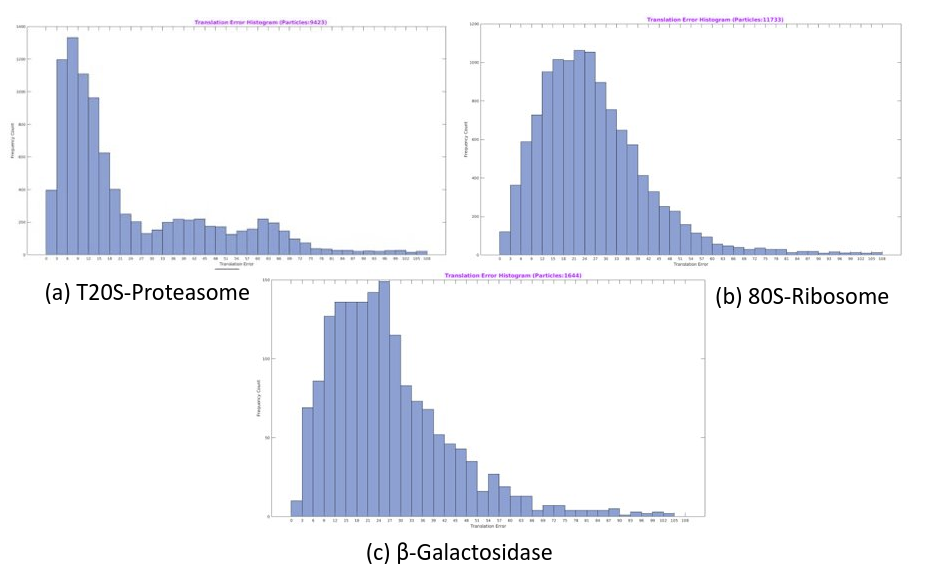
\includegraphics[width=1\linewidth]{rf-all-Translation_Error_Histogram.png}
\centering
\captionsetup{justification=centering}
\caption{Random Forest-Translation Error Histogram}
\label{fig: RF-Translation_Error_Histogram}
\end{figure}

\noindent\\
Table \ref{tbl:Random-forset-result} shows the average result of the test micrographs. Apart from accuracy, the translation error is also very important. More the translation error higher will be the reconstruction error. So, the table shows the minimum, average, maximum and median translation error. Figure \ref{fig: RF-Translation_Error_Histogram} shows the translation error histogram of all the particles. From the histogram, one can conclude that there are only few particles having translation error more than 40 pixels. On an average, approx. 25 pixel is an average translation error for all the datasets. 

\begin{figure}[H]
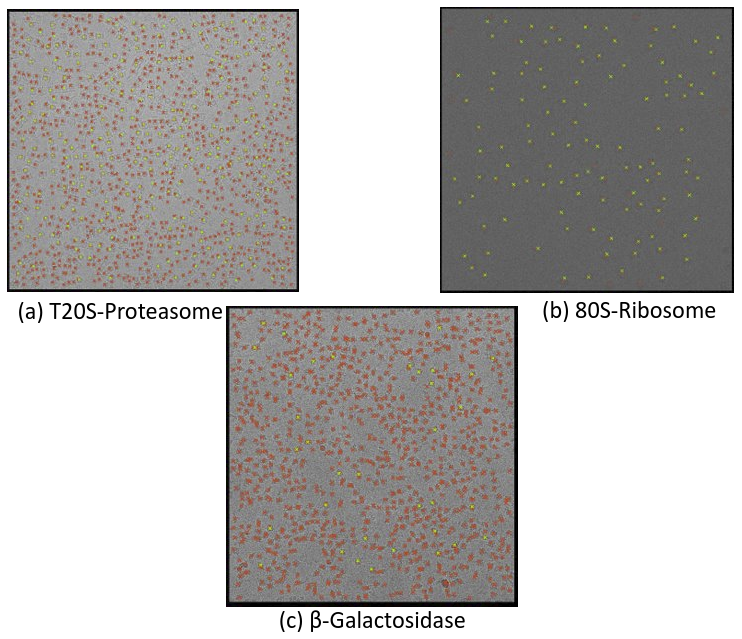
\includegraphics[width=0.98\linewidth,height=10cm]{rf-all-result.png}
\centering
\captionsetup{justification=centering}
\caption{SVM- Particle marking Results. Red: Predicted location. Green: Ground Truth}
\label{fig:RF-micrograph-marking}
\end{figure}

Micrographs \ref{fig:RF-micrograph-marking} shows the particle marking on the test micrograph for all the datasets. Red mark is the predicted location by the Random Forest classifier and green is ground truth location. One thing has be to be noted that our classifier also marked other particles for which ground truth locations were unknown. Because of this, the precision of the model is very low. But if marking for all the particles in micrograph are known then precision of the model will be good. In case of 80S-Ribosome, dataset has marking for almost all the particles that's why its precision (table \ref{tbl:Random-forset-result}) is very good as compared to other dataset.


\subsection{Classifier - Faster-RCNN}
Faster-RCNN is a variant of \textit{Region based Convolution Neural Network}. It consists of two parts, first is the Region proposal Network (RPN) and  another is the classifier and regression network. Region proposal Network gives the probable area of where object can be present and output of this layer goes to classifier and regression network for classifying the region and finding the bounding box respectively. Unlike SVM and Random Forest, for training Faster-RCNN, the input data format is different. It requires image with bounding box (top left, top right, height, width) positions of the particle. Datasets T20S-Proteasome and 80S-Ribosome have x,y coordinate rather bounding box. See section \ref{subsec:gen-train-test-faster-rcnn} for how to generate train and test datasets.

\begin{figure}[H]
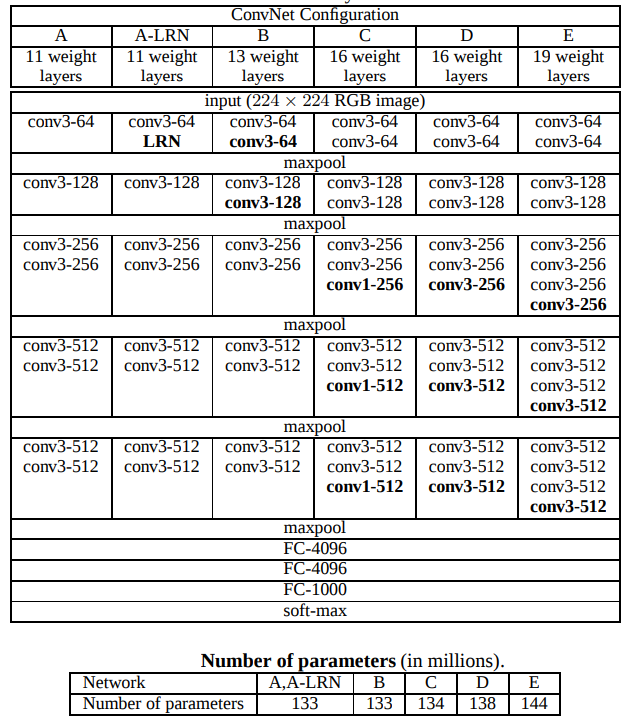
\includegraphics[width=0.6\textwidth,height=10cm]{vgg16_arch.png}
\centering
\captionsetup{justification=centering}
\caption{VGG-16: D column represent VGG-16 architecture}
\label{fig:fastercnn-vgg16-arch}
\end{figure}


\noindent\\
Faster-RCNN was trained using 4000 sub-micrographs of dimension (1000x1000) where each micrograph had approx. 3 to 4 particles bounding box marked. So, in total, number of particles were 15,831 for T20S-Proteasome dataset during training and for testing 40 micrographs (7420x7670). Firstly, a simple model with 11 layers CNN network was created and trained using downsampled sub-micrograph. Downsampled rate was 2, which means each 1000x1000 micrograph was downsampled to 500x500 before giving to network. After training this first model, it gave the accuracy of 54\%. Then, second model was created by using transfer learning of AlexNet and VGG-16 \cite{vgg16_simonyan2014very} (D column of table in figure \ref{fig:fastercnn-vgg16-arch}). Initial weights used for AlexNet and VGG-16 were the weights when these model were trained using ImageNet\footnotetext{\label{fn:ImagNet} ImageNet: http://image-net.org/}. After training approximately for 5 hrs, accuracy obtained was around 2\% from both the network which is extremely poor. There might be two probable reasons, firstly large amount of data is required to train the model as network is large and also it is pre-trained on ImageNet which do not have any class related to biological particle, more over these are tomographic projections. Secondly, the quality of input images i.e. input images are highly noisy and dark (see image (a) in figure \ref{fig: fasterrcnn-inputimage}). 


\begin{figure}[H]
\centering
\begin{subfigure}{.5\linewidth}
\centering
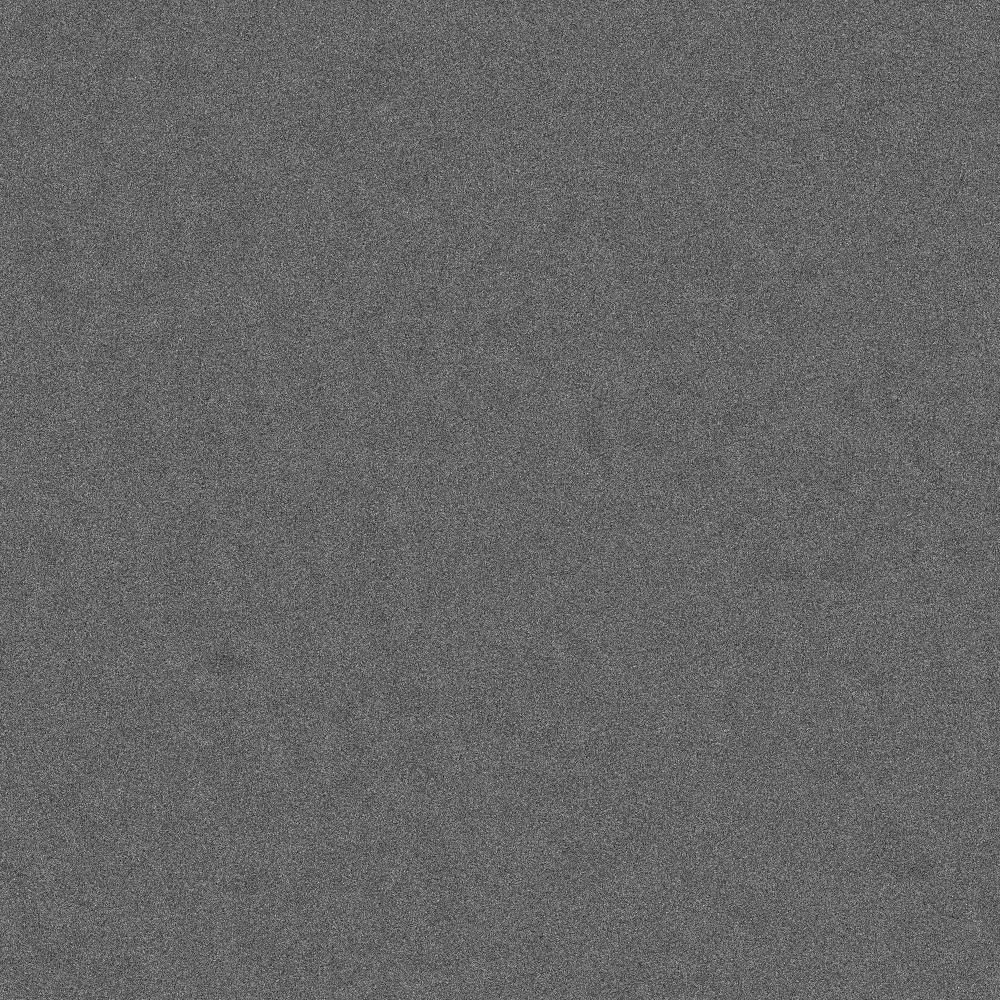
\includegraphics[width=0.5\linewidth]{fasterrcnn-input-no-prepocess.jpg}
\captionsetup{justification=centering}
\caption{ Before Pre-Processing}
\end{subfigure} 
\begin{subfigure}{.48\linewidth}
\centering
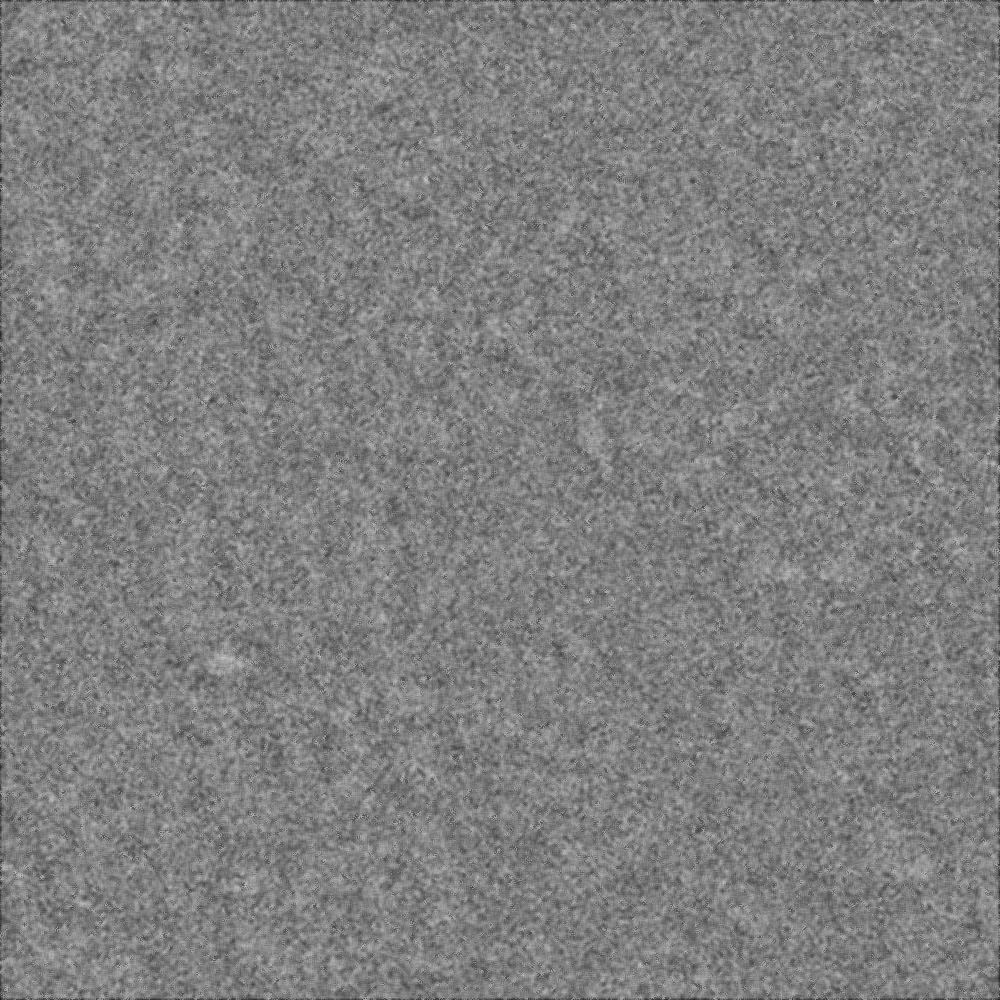
\includegraphics[width=0.5\linewidth]{fasterrcnn-input-with-prepocess.jpg}
\captionsetup{justification=centering}
\caption{ After Pre-Processing}
\end{subfigure}
\captionsetup{justification=centering}
\caption{ T20S-Proteasome: Sub-Micrograph (1000x1000). Pre-Processing includes Complement, Contrast enhancement and Noise Removal}
\label{fig: fasterrcnn-inputimage}
\end{figure}

\begin{figure}[h]
\centering
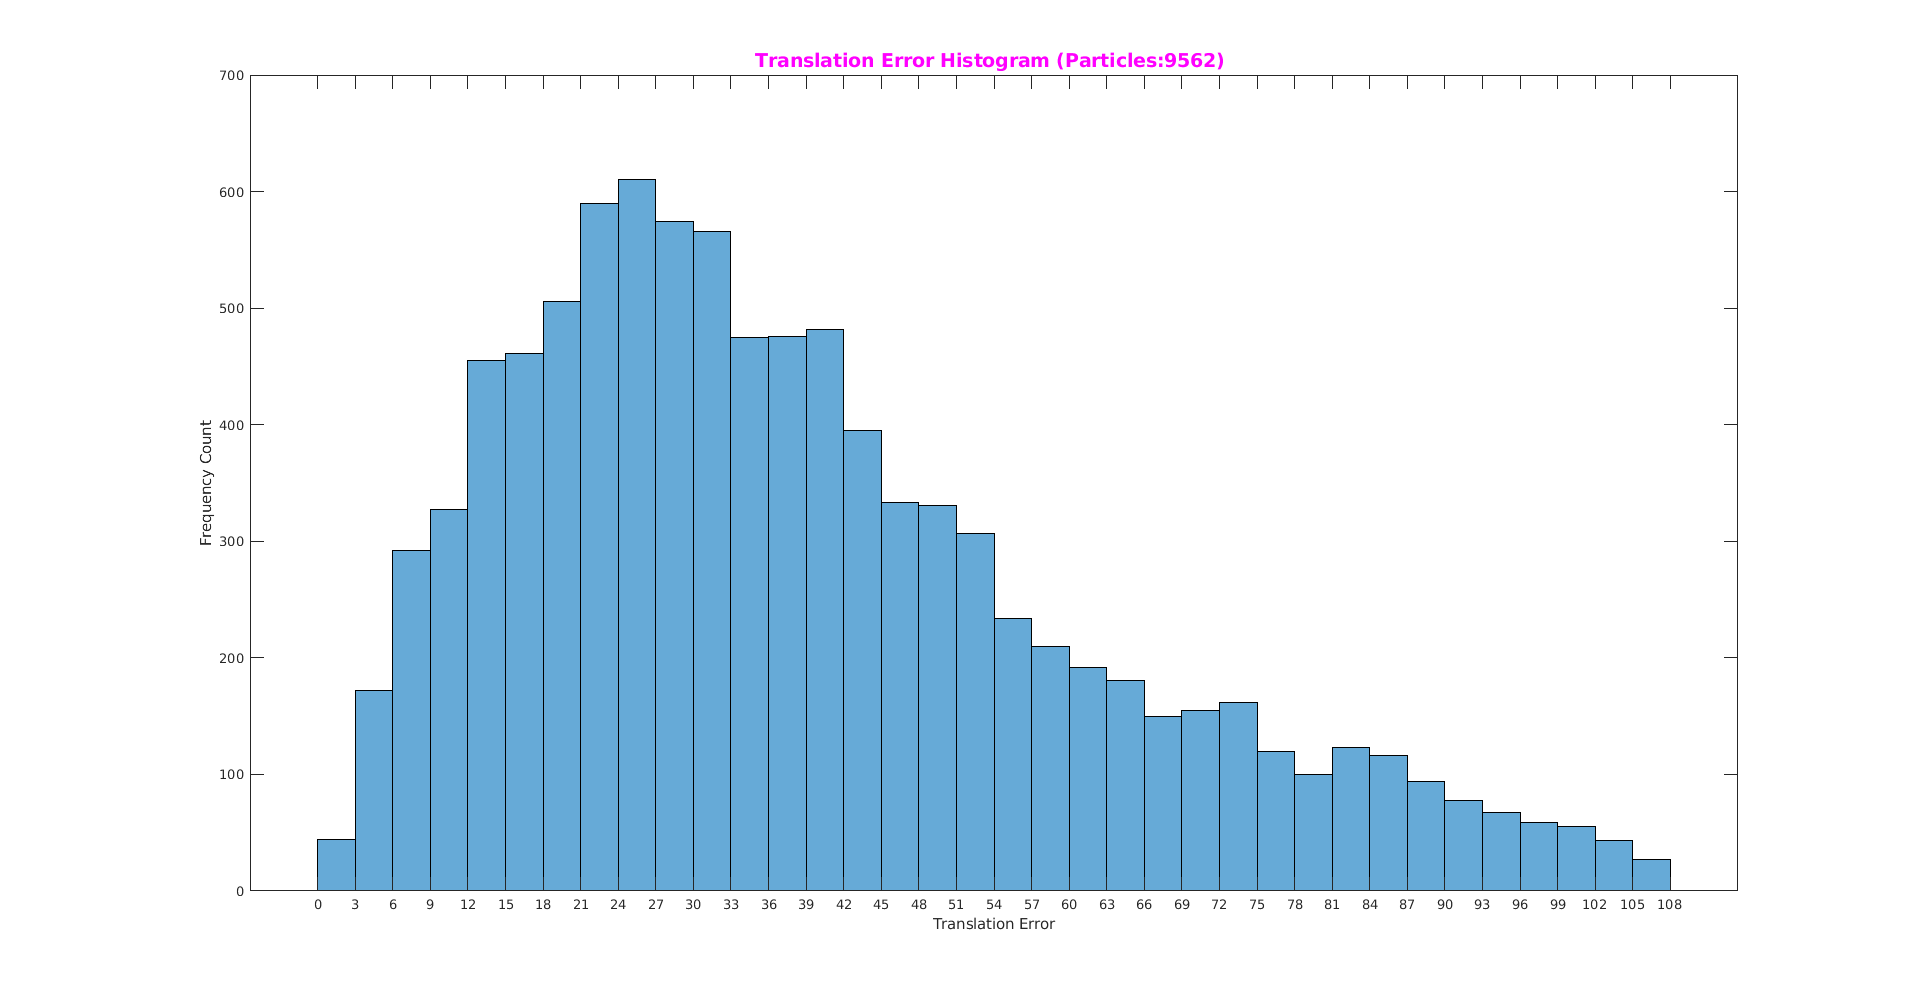
\includegraphics[width=0.68\linewidth]{fasterrcnn-EM10025-Translation_Error_Histogram.png}
\captionsetup{justification=centering}
\caption{ T20S-Proteasome: Translation Error Histogram}
\label{fig: fasterrcnn-T20S-Proteasome-Translation_Error_Histogram}
\end{figure}

In paper \cite{xiao2017fastrcnn}, for training \textit{Fast-RCNN}, contrast enhancement is done on input image before feeding to the network for reducing darkness affect. On the similar line, in our case each sub-micrograph is first passed through three level of pre-processing. First is the \textbf{complement} of the each image i.e each image is a gray scale image (i.e. one channel image) so in case of gray scale after doing the complement white will become black and vice-versa. The second step was to increase the contrast and for that \textbf{Histogram Equalization} method is used. The third and last step is to reduce the level of noise so for that \textbf{Wiener} filter of 5x5 is used using the mean of the local variance.

\subsubsection{Result}
Faster-RCNN was trained on one dataset which was T20S-Proteasome with 1000x1000 sub-micrographs using VGG-16 architecture. VGG-16 had 41 layers including the input and last layer. The learning parameter was set to $1\times e^{-5}$. For anchor configuration, see table \ref{tbl:FasterRCNN-result}. The complete training took around 4 hrs using the pre-processed downsampled-by-4 sub-micrographs. 

\begin{table}[H]
\centering
  \begin{tabularx}{\textwidth}{|*{7}{Y|}}
    \hline\hline
    \multirow{2}{*}{Dataset} &\multirow{2}{*}{Recall} & \multirow{2}{*}{Precision} &\multicolumn{4}{c|}{Translation error (pixel)}\\
    \cline{4-7}
             & & & min. & max. & avg. & median \\
    \hline
T20S & 96\% & 6\% & 0 & 108 & 39 & 34 \\ \hline
\hline
\end{tabularx}
\caption{Faster-RCNN Result}
\label{tbl:FasterRCNN-result}
\end{table}

Testing was performed on 40 micrograph each of dimension 7420x7670. During testing phase, when full micrograph (7420x7670) was directly passed then accuracy was poor. As the model was trained on 1000x1000 sub-micrographs which further downsampled by 4. So while testing, each test micrograph was divided into sub-micrographs of size 1000x1000 and then downsampled at 3 scale which were 4,3,2 before giving it to Faster-RCNN. Results of all the micrograph was then assembled into one and duplicated markings were removed using NMS (Non-Minimal Suppression). This gave the average accuracy of 40 micrographs as 96\% and detection time was just 1.5 mins which was much better than SVM and Random Forest.

\begin{figure}[H]
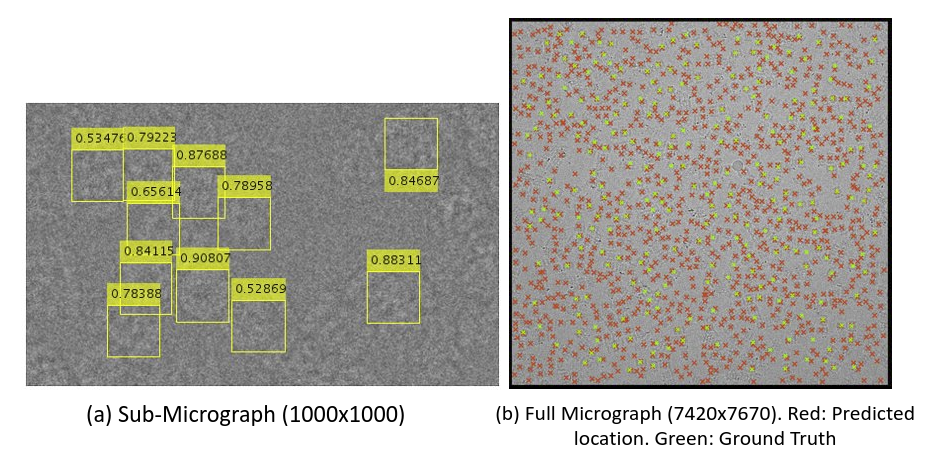
\includegraphics[width=1\linewidth]{fasterrcnn-result-T20.png}
\centering
\captionsetup{justification=centering}
\caption{Faster-RCNN - T20S-Proteasome Result}
\label{fig: fasetrcnnT20S-Proteasome-Result}
\end{figure}


\noindent\\
Observation is that doing the pre-processing before giving to VGG-16 gives better result as compared to without pre-processing. When VGG-16 model was trained without pre-processing then accuracy obtained was approximately 2\% but when pre-processing i.e. complement, contrast enhancement and noise reduction was performed then average result from V66-16 was 96\%.

\subsection{Conclusion}

Three types of Particle-Picker are created using SVM, Random Forest and Faster-RCNN. In terms of \textit{accuracy (Recall)}, all performed very well i.e. above 90\%. With respect to 
\textit{precision} on current dataset, Random Forest based model performed very well. But, judging any model based on \textit{precision} \cite{wang2016deeppicker} \cite{xiao2017fastrcnn} for the current dataset will not be right as there are lots of particles for which markings are not present during the experiment. That means, precision is not the right parameter to judge the model. Another important parameter is \textit{translation error} which is very important parameter w.r.t. 3D reconstruction i.e. less the translation error more right will be 3D reconstructed model. Here, Faster-RCNN (table \ref{tbl:FasterRCNN-result}) has average translation error of 39 pixels which is more than other two models. Between SVM (table \ref{tbl:SVM-result}) and Random-Forest (table \ref{tbl:Random-forset-result}), Random Forest has little less translation error. When parameter \textit{detection time} is considered then Faster-RCNN is best because it took only 1.5 mins to test one 7420x7670 micrograph. On the other hand SVM took 25-30 mins. But CPU based Random Forest took 2-3 hrs. For the same size of micrograph which is very large time as compared to other two model. \\


Deciding which model is best just by one parameter will not be right. Its a mixture of accuracy, precision, translation error and detection time. An ideal model should have very high accuracy and precision. On the other hand, model should have very low translation error and detection time. Considering these datasets and these three models (SVM, Random Forest and Faster-RCNN) then, Faster-RCNN is doing very well because in terms of accuracy and detection it is better than other two. Precision parameter is not considered as markings are incomplete. And for translation error, approximately 15 pixel difference is there between Faster-RCNN and other two (SVM and Random Forest) which is not very large. But Random Forest is better than Faster R-CNN w.r.t. marking errors and translation errors. Because Faster R-CNN has marked many particles which are not actually a particle (in visual sense), also it has very large translation error. Quantitatively which model is better can only be decided when ground truth for all the particles are known. 

\chapter{3D Reconstruction}
The reason for doing particle picking is to 3D reconstruct the molecule using those markings. After the particle picking and before 3D reconstruction, there are few more steps involved such as Clustering, CTF correction, etc. (see section \ref{sec: basic_pipeline}). 3D reconstruction is a challenging job because the angles and shifts of the projections are unknown. Without knowing the angles as well as shifts, right reconstruction is near to impossible. Tools like RELION uses the Bayesian \cite{scheres2012relion} approach for solving this problem and optimizes the equation in alternating fashion, i.e. by finding the rough estimate and then performing the back-projection (reconstruct the object). After that, it performs the forward projection at those angles for calculating the error, and this process is repeated. \\

Performing 3D parallel beam filtered back-projection becomes harder because of unavailability of libraries. For 2D parallel beam filtered back-projection, radon and iradon are available. But in case of 3D, things get more challenging because of the parallel beam, as in the field of tomography cone beam is widely used but the parallel beam is used only in few applications such as in electron microscope. But there is a toolbox name \textit{ASPIRE} developed by A.Singer and group from Princeton University and \textit{TIGRE} developed by CERN which can perform "3D parallel beam filtered back-projection". The next section will talk about the ASPIRE and TIGRE toolboxes features and how these can be used for 3D reconstruction.

\section{ASPIRE}

ASPIRE\protect\footnotemark\footnotetext{ASPIRE: http://spr.math.princeton.edu/} stands for "\textbf{A}lgorithms for \textbf{S}ingle \textbf{P}art\textbf{i}cle \textbf{Re}construction". This toolbox is developed by then Amit Singer and his group of Princeton University for the use of Cryo-EM. This toolbox supports the parallel beam 3D radon reconstruction along with the common line and angle estimate for the single-particle projections and many more features. 

ASPIRE is a good toolbox to start with, but it has one major drawback. For a 3D reconstruction of the object of size 64x64x64 with 500 projections, given angles, ASPIRE takes minutes (approx. 20 to 30 min or more depending on the computer). The 3D reconstruction doesn't use the GPU for faster reconstruction, which makes this library hard to used for making fast algorithms. 

\section{TIGRE ing the correct angle and shift assignments.
Toolbox}\label{subsec:TIGRE}
TIGRE\protect\footnotemark\footnotetext{TIGRE: https://github.com/CERN/TIGRE} stands for "\textbf{T}omographic \textbf{I}terative \textbf{G}PU-based \textbf{Re}construction Toolbox". As the name suggests, it uses GPU (Graphical Processing Unit) for reconstruction. 3D reconstruction is computationally expensive so, if GPU is not used, then it will take many hours depending on the dimension of the object to be constructed. For reconstructing the 3D model of dimension 160x160x160 using 100 projections, TIGRE took only a few seconds, which is very good w.r.t ASPIRE. One thing that has to be considered while reconstructing is that bigger the dimension, larger will be the reconstruction time and main memory (RAM + GPU) required will be more. \\

\begin{figure}[H]
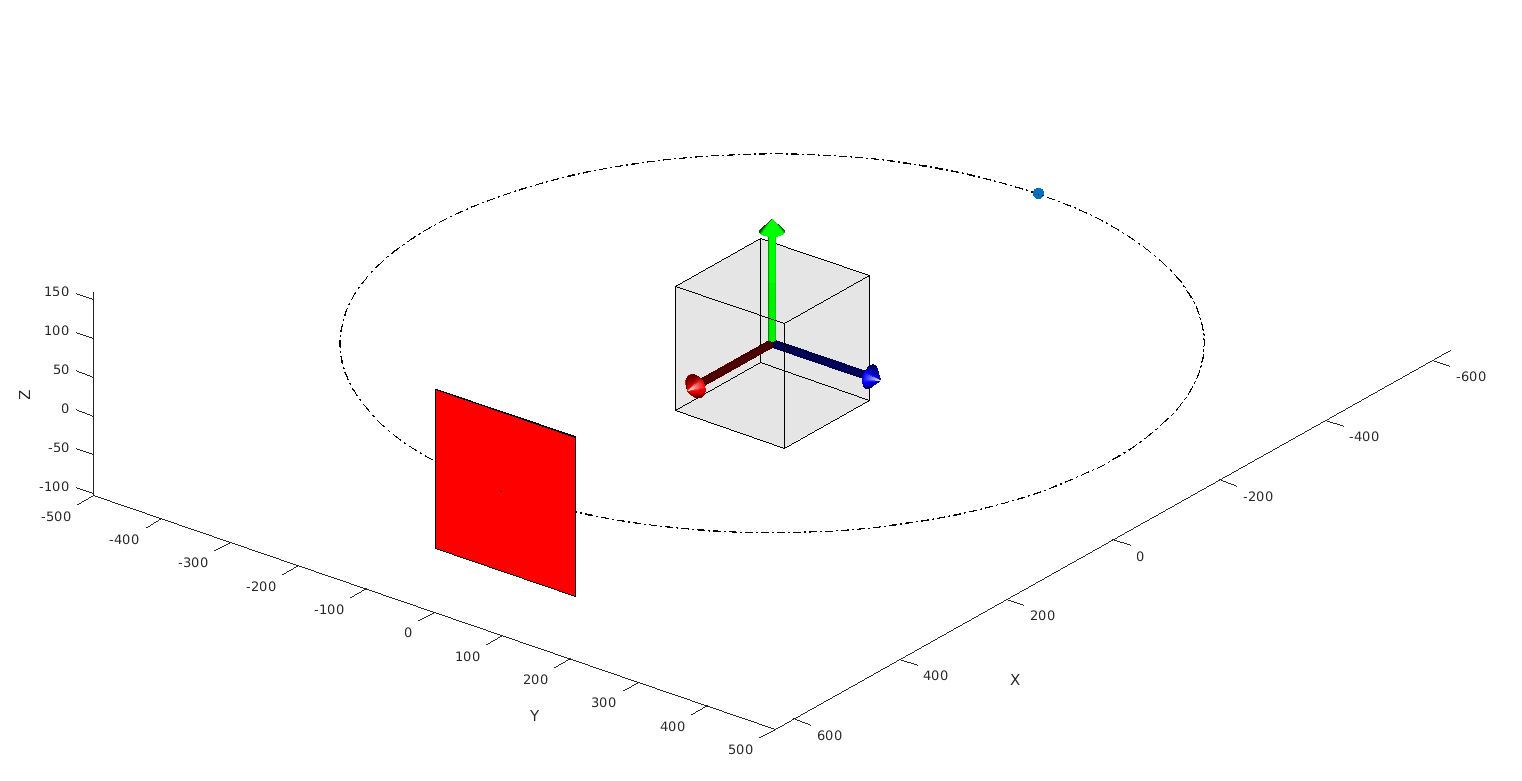
\includegraphics[width=1\linewidth]{tigre_projection_geomtery.png}
\centering
\captionsetup{justification=centering}
\caption{Figure represent placement of object, source and detector. Detector is at distance 1000 mm and  source is at 500 mm. Blue dot represent the source and Red quadrilateral is detector.}
\label{fig: tigre_projection_geomtery}
\end{figure}

TIGRE toolbox has many libraries for parallel beam as well as cone beam but in our application parallel beam is required, as the electron microscope uses parallel beam. Before acquiring projections or 3D reconstruction, one needs to create "geometry". In the case of acquiring projections, "geometry" will have information related to source distance and detector distance from the object when the object is placed at origin (see image (\ref{fig: tigre_projection_geomtery}) ). Geometry will also have information related to detector dimension, detector pixel size, the accuracy of interpolation, and the dimension of the object. By using library function $Ax (object, geometry, angles, 'interpolated')$ of TIGRE, projections at the specific angle can be taken. For 3D reconstruction one can use library function $FBP(projections, geometry, angles)$ for filtered back-projection and  BP (Back-Projection) one can use "Atb (projections, geometry, angles)". \\

Next section will talk about our proposed algorithm for finding angles and shift of the projections. Once these are known,  then using TIGRE library function reconstruction can be done.

\section{Proposed Algorithm}\label{sec: Proposed_Algorithm}
This algorithm does not uses the Bayesian approach like RELION \cite{scheres2012relion}; it's correlation based optimization. Our algorithm is divided into four major parts, i.e., noise removal from projections, common line estimate, angle initialization, and correlation optimization algorithm for find

\subsection{Noise Removal} \label{subsec: noise-removal from projection}

In Cryo-EM, micrographs and projections are highly noisy. They are so noisy that without doing any pre-processing on micrographs, seeing projections perfectly with naked eyes are near to impossible. That's why biologist does not prefer crowdsourcing of particle picking \cite{bruggemann2017exploring} much. Also, if noisy projections are used for 3D reconstruction, then the reconstructed object will also be noisy, and there is a high possibility that the object will be wrongly constructed. As for 3D reconstruction, angles and shifts for projections should be known. But here, these are unknown initially. So, before reconstruction, initial angles and shifts are computed using the projections. If projections are noisy, then estimated angles and shifts will not perfect, which further leads to the wrong reconstruction. 

There are various ways this noise can be removed. One of the most popular ways is to use clustering \cite{mallick2006structure}. But for clustering to work, there is a need of 30 to 50 thousands of projections. Larger the number projections larger will be the probability that more projections will lie in one cluster. More the number of projections per clusters less noisy will be the averaged projection. Another way for removing the noise is to use the Wiener filter, BM3D method, etc.

\subsubsection{BM3D}\label{subsubsec:BM3D}
BM3D \cite{dabov2009BM3D}\cite{lebrun2012BM3Danalysis} is the collaborative filtering for the noise removal for 2D image. It is a two step noise reduction algorithm. It is a patch based algorithm and each stage is divided into the four modules :
\begin{enumerate}
  \item Finding the similar patches to a given patch in the image and collaborate it in a 3D matrix or block
  \item 3D Linear transformation of the 3D block
  \item Shrinkage the transform coefficients also called as Thresholding or perform the Wiener filtering
  \item 3D inverse transformation
\end{enumerate}

The only difference between the two stages is the third module, i.e., in first step thresholding is used and in the second step, Wiener filter is used (refer the figure (\ref{fig: bm3d}) ). Step 1 is first executed on the whole image, and then step 2 is performed. After each step, the 3D filtered patch is obtained, which the reassigned to its original location. As overlapping patches are used, each pixel has multiple values. So to handle the overlapping case, \textit{aggregation} is performed at each pixel. BM3D works on the fact that the image has a sparse local representation in the transformation domain. Also collaborative filtering reveals the finest detail shared by the similar patches.


\begin{figure}[h]
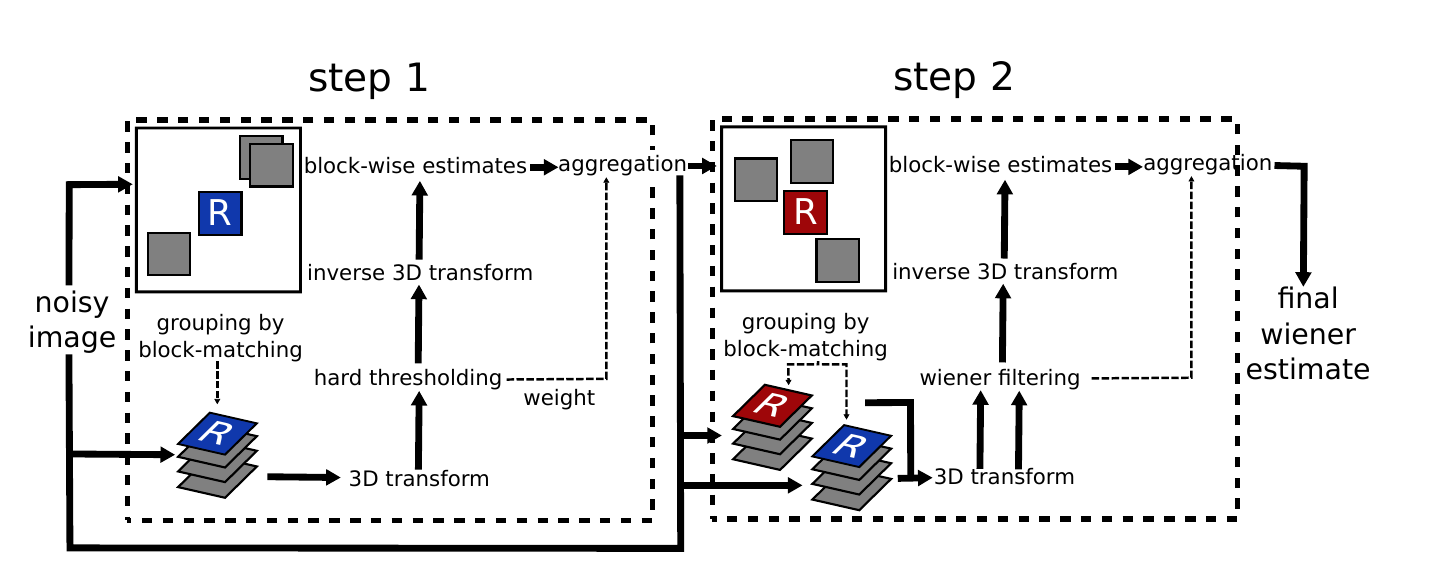
\includegraphics[width=0.9\linewidth]{bm3d.png}
\centering
\captionsetup{justification=centering}
\caption{ BM3D Algorithm Pipeline Source: \cite{lebrun2012BM3Danalysis} }
\label{fig: bm3d}
\end{figure}

For noise removal, in our experiments, BM3D is used for Gaussian noise removal instead of the clustering. As clustering based noise removal require a large number of projections. Also, if one is using K-Means clustering, then the image cannot be used directly because the image is a 2D matrix, but K-Means with L2 norm or cosine distance requires vector. Using raw images in K-Means with L2 norm or cosine distance will leads to lose of spatial information.  So, to overcome that, one has to use features from images in K-Means rather than the raw images.

\subsection{Common Line}

Projections from Cryo-EM are noisy and have unknown angles and shifts. Unknown angle problem arises due to the random orientation of Bacteria/Virus/Ribosome etc. in the sample under study. And the unknown shift problem arises due to the wrong center marking of the projections in the micrograph. Also, reconstruction required angles and shifts to be known. So for the rough initial estimate of the angles and shifts, prior information related to projections can be used. 

In the case of 3D, one can do a smarter initialization by exploiting the properties of 3D geometry. Fourier slice theorem (\ref{sec:for_slice_theorem}) says that if object is 3D and its 2D projection is taken at some angle say $(\alpha,\beta,\gamma)$, then Fourier transform of that 2D projection will be equal to the slice passing through the origin  at angle $(\alpha,\beta,\gamma)$ of the Fourier transform of the 3D object. Fourier slice theorem gives the key information in relation with angle initialization. Let's consider there are two 2D projections 1 \& 2 taken at different angles. Take the Fourier transform of these two projections. Now by Fourier slice theorem, a relative slice of projection 1 \& 2 in the Fourier domain of the 3D object will pass through the origin. Assuming these two slices are non-coplanar then these two slice will intersect at a line which is called as \textit{common line} \cite{mallick2006structure} \cite{van1987angular} (see figure \ref{fig: 3dr_plane_intersection}). This logic can be extended to any number of projections, but the only constraint is that they should be non-coplanar. \\

\begin{figure}[h]
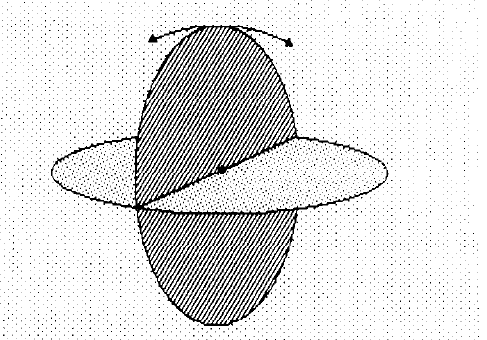
\includegraphics[width=0.7\linewidth]{3dr_plane_intersection.png}
\centering
\captionsetup{justification=centering}
\caption{Common line: Intersection of Fourier slice of two projections in Fourier Space. Black dot represent the origin of the Fourier Space. Source:  \cite{van1987angular} }
\label{fig: 3dr_plane_intersection}
\end{figure}

Finding a common line between two projections will help in finding the rough initial angle estimate of projections. Let the common line between the projection ${p_i}$ \& ${p_j}$ is denoted by ${c_{ij}}$. ${\phi_{ij}}$ denotes the angle made by the common line ${c_{ij}}$ with the local coordinates system of the projection ${p_i}$. Similarly, ${\phi_{ji}}$ denotes the angle made by the common line ${c_{ij}}$ with the local coordinates system of the projection ${p_j}$. 

\[\label{eq:commonline_phi}
\Phi
=
\begin{bmatrix}
    \phi_{11} & \phi_{12} & \phi_{13} & \dots  & \phi_{1n} \\
    \phi_{21} & \phi_{22} & \phi_{23} & \dots  & \phi_{2n} \\
    \vdots & \vdots & \vdots & \ddots & \vdots \\
    \phi_{n1} & \phi_{n2} & \phi_{n3} & \dots  & \phi_{nn}
\end{bmatrix}
\]

For computing ${\phi_{ij}}$, common line between the projections  ${p_i}$ \& ${p_j}$ needs to be find out. Finding a common line can be done in the Fourier domain or in the spatial domain. For finding a common line in the spatial, below steps can be followed:


\begin{enumerate}
    \item Define the angle search space meaning up to what accuracy level of decimal precision in ${\phi_{ij}}$ you want. For simple understanding, assume ${\phi_{ij}}$ to be integer rather than real. 
    \item Divide the angles from 0 to 360 by 1 degree. So we will get 360 angles, let's call it ${n}$ angles.
    \item Take 1D Radon transform for ${p_i}$ \& ${p_j}$ at all these ${n}$ angles. These 1D projections are following the principle of Fourier slice theorem. Working in a spatial domain helps in avoiding complex number, also for interpolation in Fourier domain one is required to use NUFFT (nonuniform fast Fourier transform) \cite{fessler2003NUFFT}.
        
     \item Create a ${nxn}$ matrix, here it will be ${360x360}$ normalized correlation matrix. Where, each ith row denotes the ith degree starting from $0^{\circ}$  with increment by 1 (search space is a hyperparameter), similarly for the jth column. Each $ij$ denotes the normalized correlation of the ${i_th}$ 1D radon projection for ${p_i}$  with the ${j_th}$ 1D  radon projection of the ${p_j}$   
    
    \item Find the $ij_th$ entry for which normalized correlation value is the maximum. That  $ij_th$ entry, ${i_th}$ row angle will be the $\phi_{ij}$ and ${j_th}$ column angle will be the $\phi_{ji}$
\end{enumerate}

\subsection{Angle Initialization}\label{subsec: angle_initialization}
Finding projections angles using our algorithm requires some initial angles estimate for all projections at the start of the algorithm. One way to initialize angles is random initialization or use some prior knowledge about projections.\\ 
 
 By utilizing the property of common line, initial angles estimate or rotation matrix for projections can be calculated using Satya P. Mallick et al.\cite{mallick2006structure}, A. Singer et al. \cite{singer2009threeAngleEstimate} \cite{sigworthcryoAngleEstimate}, Zang et al. \cite{wang2018improvingAngleEstimate}, etc.  Our experiments uses the A. Singer et al. \cite{singer2009threeAngleEstimate}. It uses the ${\Phi}$ (see eq. (\ref{eq:commonline_phi})) for the estimation of rotation matrices instead of projections angles. But once the rotation matrix is know one can easily find out the angles. Here, in our experiments for making thing consistent at every stage \textit{Euler-XYZ} rotation representation is used (see eq. (\ref{eq:rotation_xyz})), where ${\boldsymbol{R_x}}$, ${\boldsymbol{R_y}}$ \& ${\boldsymbol{R_y}}$ means rotation about rotation x-axis, y-axis and z-axis respectively.
 
 
 \begin{equation} \label{eq:rotation_xyz}
     \boldsymbol{R}  =   \boldsymbol{R_x} \times \boldsymbol{R_y} \times \boldsymbol{R_z}
 \end{equation}
 
  \begin{equation} \label{eq:amit_commonline}
     \boldsymbol{c_{ij}}  
      =  
     \begin{bmatrix}
       \cos{\phi_{ij}} \\ 
       \sin{\phi_{ij}} \\ 
       0  
     \end{bmatrix}
 \end{equation}
 
 \begin{equation} \label{eq:amit_commonline_rot_equality}
     \boldsymbol{R_i.c_{ij}}  =   \boldsymbol{R_j.c_{ji}} \hspace{0.2cm} \forall \hspace{0.1 cm}  1\lneq i \lneq j \lneq N
 \end{equation}
 
 In \cite{sigworthcryoAngleEstimate}, below eq. (\ref{eq:amit_obj_fun}) is optimized by exploiting the fact of equality \ref{eq:amit_commonline_rot_equality}. ${\boldsymbol{R_i}}$ denotes the true rotation matrix for the projection ${p_i}$. ${\boldsymbol{c_{ij}}}$ denotes the common line between the projections ${p_i}$ \& ${p_j}$ w.r.t.  the local coordinate system of ${p_i}$, defined as eq. (\ref{eq:amit_commonline}), similarly for ${\boldsymbol{c_{ji}}}$. In eq (\ref{eq:amit_obj_fun}), if ${\boldsymbol{R_i}}$ is a true rotation matrix then maximum sum will be N, i.e., number of projections, else it will be less than that. 
 
 
 \begin{equation}\label{eq:amit_obj_fun}
  \begin{aligned}
  & \enspace \boldsymbol{\max\limits_{R_1\dots R_2}} \enspace \boldsymbol{\sum\limits_{i \neq j}} \boldsymbol{R_ic_{ij}} 	\cdot \boldsymbol{R_jc_{ji}}  \\
     &  \enspace  subject \enspace to,\\
     & \enspace  \boldsymbol{R_i}\boldsymbol{R_j} =  \boldsymbol{I} \\
     & \enspace \boldsymbol{\det{R_i}}= 1 \\
     &  \enspace  \forall \enspace i = 1,2 \cdots , N\\
  \end{aligned}
\end{equation}


Optimizing eq. (\ref{eq:amit_obj_fun}) directly is not possible. So, if certain things are assumed, i.e. some prior information, then some constraints can be relaxed, which further help in solving the equation.  Eq. (\ref{eq:amit_obj_fun}) is a quadratic in unknown rotation ${\boldsymbol{R_1}}$ ${\cdots}$ ${\boldsymbol{R_N}}$, so if constraints are relaxed properly, then solution to the optimization problem would be related to the top eigen vectors of the matrix defining quadratic form (refer  \cite{singer2009threeAngleEstimate}). 

Optimizing of eq. (\ref{eq:amit_obj_fun}) using the eigen value decomposition \cite{singer2009threeAngleEstimate}) will give the initial rotation estimate of projections, lets call this initial estimate as ${\boldsymbol{R_i^{init}}}$ for projection ${pi}$. Using this ${\boldsymbol{R_i^{init}}}$ initial 3D reconstruction is done, let call this initial 3D reconstruction as ${\boldsymbol{G^{init}}}$ and ${\boldsymbol{F}}$ been the true object.     

\subsection{Correlation Optimization}

Our \textit{Correlation Optimization} algorithm can be used for further correcting the rotation and translation estimate found in section (\ref{subsec: angle_initialization} ) for \textit{Angle Recovery Problem (ARP)} and \textit{Shift-Angle Recovery Problem (ShARP)}.  This section talks about the refinement of rotation estimate in ARP assuming no translation error and the translation and rotation estimate in ShARP. In ARP, it is assumed that there is no translation error in the projections, and they are center aligned. In ShARP, no assumptions are taken into consideration w.r.t rotation and shift.

\subsubsection{\textbf{Angle Recovery Problem}}

Angle recovery problem assumes that there is no translation error, so only orientations for projections will be estimated. Our algorithm tries to optimize the eq. \ref{eq:our_obj_fun_arp} iteratively for all projections till convergence. In eq. (\ref{eq:our_obj_fun_arp}), ${\boldsymbol{NCor(x,y)}}$ will finds out the \textit{normalized correlation} between the image ${x}$ \& ${y}$. ${\boldsymbol{Radon(G,ang_{1\times 3})}}$ will find out the 3D radon transform of the 3D object ${G}$ at the given angle ${ang_{1 \times 3}}$.    


\begin{equation}\label{eq:our_obj_fun_arp}
  \begin{aligned}
    (\theta^1_i,\theta^2_i,\theta^3_i)  = & \hspace{0.1cm} argmax_{\theta^1,\theta^2,\theta^3} \hspace{0.1cm} \boldsymbol{NCor(}  p_i^{true}\hspace{0.1cm} , \hspace{0.1cm} \boldsymbol{Radon(G}, [ \alpha+\theta^1,\beta+\theta^2,\gamma+\theta^3 ] \boldsymbol{)} \boldsymbol{)}\\
    & where,\\
    &  -k \lneq \theta^1 \lneq k\\
    &  -k \lneq \theta^2 \lneq k\\
    &  -k \lneq \theta^3 \lneq k\\
    &  \forall \enspace i = 1,2 \cdots , N\\
    & \alpha : angle\hspace{0.1cm}with\hspace{0.1cm}x-axis,\\
    & \beta : angle\hspace{0.1cm}with\hspace{0.1cm}y-axis,\\
    & \gamma : angle\hspace{0.1cm}with\hspace{0.1cm}z-axis,\\
    &  k : search\hspace{0.1cm}area\hspace{0.1cm}hyperparameter \\
    & N: number\hspace{0.1cm}of\hspace{0.1cm}projections\\
  \end{aligned}
\end{equation}

Algorithm (\ref{algo:our_arp}) tells, how to solve optimization eq. (\ref{eq:our_obj_fun_arp}) as a closed form solution does not exist. So for solving this, iterative approach is used. The only hyperparameter is ${k}$, which will define the final angles predictions. If the initial estimates are very good, then the value of ${k}$ can be less. But if the initial angle estimate is bad, then the large value for ${k}$ can be set. Value of ${k}$ defines the execution time of the algorithm, i.e., if the ${k}$ is very large then just to complete one iteration for all ${N}$ projections, it will take a lot of time. So, it's advisable to set ${k}$ to 5 to 10 because even if the initial estimate is bad, the algorithm will reach its convergence but slowly.\\ \\  


\begin{algorithm}[H]
\caption{ARP}
\SetAlgoLined
\KwIn{ All ${\boldsymbol{P}}$ projections, ${\boldsymbol{G^{init}}}$, ${\boldsymbol{R^{init}_i}}$ \& k }
\KwOut{ Returns estimated ${\boldsymbol{G^{est}}}$ \& ${\boldsymbol{R^{est}_i}}$}
 \textbf{Initialization:} \\ 
 ${\boldsymbol{G^{est}}}$ = ${\boldsymbol{G^{init}}}$ \\
 ${\boldsymbol{R^{est}_i}}$ = ${\boldsymbol{R^{init}_i}}$ \\
 \While{till convergence}{
  \While{i: 1 ${\rightarrow}$ N}{
    \hspace{0.1cm} ${\alpha,\beta,\gamma}$  = $\boldsymbol{Rot2Euler}$ ( ${\boldsymbol{R^{est}_i}}$) \\
    \begin{equation*}
        \begin{aligned}
            \hspace{-1.5cm} (\theta^1_i,\theta^2_i,\theta^3_i)  = & \hspace{0.1cm} argmax_{\theta^1,\theta^2,\theta^3}\\
            & \hspace{0.1cm} \boldsymbol{NCor(}  p_i^{true}\hspace{0.1cm} , \hspace{0.1cm} \boldsymbol{Radon(G^{est}}, [ \alpha+\theta^1,\beta+\theta^2,\gamma+\theta^3 ] \boldsymbol{)} \boldsymbol{)} \\
            & where,\hspace{0.1cm} -k \lneq \theta^1,\theta^2 ,\theta^3 \lneq k\\
        \end{aligned}
    \end{equation*}
    \hspace{0.5cm} ${\boldsymbol{R^{est}_i}}$  =  $\boldsymbol{Euler2Rot}$ ( ${[ \alpha + \theta^1_i,\beta + \theta^2_i,\gamma +  \theta^3_i ]}$ )\\
   }
   ${\boldsymbol{G^{est}}}$ = \textbf{invRadon} ( ${P^{true}_{1\cdots N}}$, ${\boldsymbol{R^{est}_{1 \cdots N}}}$)\\ 
   \vspace{0.1cm}
   ${P_{1\cdots N}}$ = \textbf{Radon} ( ${\boldsymbol{G^{est}}}$, ${\boldsymbol{R^{est}_{1 \cdots N}}}$)\\
   \vspace{-0.55cm}
   \begin{equation} \label{eq:our_arp_correaltion_error}
        \begin{aligned}
         \hspace{-6.60cm} error = \textbf{NCor}(P_{1\cdots N},P^{true}_{1\cdots N})
         \end{aligned}
    \end{equation}
 }
\label{algo:our_arp}
\end{algorithm} 

\hspace{1cm}\\
The algorithm (\ref{algo:our_arp}) is divided into two parts, first is to use the estimated reconstructed the object for finding the approximately correct angles of projection, and second is to use the estimated projections angles for reconstructing the object back using the true projections. This process is repeated till convergence, i.e., until there is no change in the estimated projections angles or rate of change of \textit{error} is very small. Final ${\boldsymbol{G^{est}}}$ is the final reconstructed object. 


\subsubsection{\textbf{Shift-Angle Recovery Problem}}

ShARP optimization problem does not assume anything on projections angles and shifts error. Shift error is introduced at the particle picking stage irrespective of the method used. Automated, as well as the manual methods of marking projections in the micrograph,  are not 100 percent perfect, i.e., projections will be shifted by some pixels from their true center. So for 3D reconstruction, the shifts should also be known along with the angles else reconstruction will not be possible. If anyhow marked projections are perfect, i.e. without any shift error then ARP algorithm \ref{algo:our_arp} can be used instead of ShARP algorithm.  

ShARP algorithm tries to optimize the eq. (\ref{eq:our_obj_fun_sharp}) for projection angles and their shift simultaneously.  In eq. \ref{eq:our_obj_fun_sharp}, ${\boldsymbol{NCor(x,y)}}$ will finds out the \textit{normalized correlation} between the image ${x}$ \& ${y}$. ${\boldsymbol{Radon(G,ang_{1\times 3})}}$ will find out the 3D radon transform of the 3D object ${G}$ at the given angle ${ang_{1 \times 3}}$. ${\boldsymbol{Shift(img,[t_x,t_y])}}$ will shift the image ${img}$ by ${t_x}$ in x-axis and ${t_y}$ in y-axis from the origin. In our all experiments, origin is considered to be center of the projections.   

\begin{equation}\label{eq:our_obj_fun_sharp}
  \begin{aligned}
    (\theta^1_i,\theta^2_i,\theta^3_i)  = & \hspace{0.1cm} argmax_{\theta^1,\theta^2,\theta^3} \hspace{0.1cm} \\ &\boldsymbol{NCor(}\hspace{0.1cm}\boldsymbol{Shift} ( p_i^{true} , [t_x,t_y])\hspace{0.1cm} , \hspace{0.1cm} \boldsymbol{Radon(G}, [ \alpha+\theta^1,\beta+\theta^2,\gamma+\theta^3 ] \boldsymbol{)} \boldsymbol{)}\\
    & where,\\
    &  -k \lneq \theta^1,\theta^2,\theta^3 \lneq k\\
    &  \forall \enspace i = 1,2 \cdots , N\\
    & \alpha : angle\hspace{0.1cm}with\hspace{0.1cm}x-axis,\\
    & \beta : angle\hspace{0.1cm}with\hspace{0.1cm}y-axis,\\
    & \gamma : angle\hspace{0.1cm}with\hspace{0.1cm}z-axis,\\
    & t_x : shift\hspace{0.1cm}in\hspace{0.1cm}x-axis,\\
    & t_y : shift\hspace{0.1cm}in\hspace{0.1cm}y-axis,\\
    &  k : search\hspace{0.1cm}area\hspace{0.1cm}hyperparameter \\
    & N: number\hspace{0.1cm}of\hspace{0.1cm}projections\\
  \end{aligned}
\end{equation}


Eq. (\ref{eq:our_obj_fun_sharp}) do not have any closed form solution, so interactive approached is used for finding the probable solution. ShARP algorithm is somewhat similar to the ARP algorithm (\ref{algo:our_arp}) except the shift estimation. For estimating the shifts, \textit{Cross-Power Spectrum} \cite{reddy1996fft} is used. Cross-Power spectrum methods will perfectly tells the shift between images. Let say there are two  images ${f_1}$ \& ${f_2}$ which is given by translation eq. (\ref{eq:translation}) then cross-power spectrum of ${f_1}$ \& ${f_2}$ will give the shifts i.e ${t_x}$ \& ${t_y}$. 

\begin{equation}\label{eq:translation}
    f_1 (x,y) = f_2 (x-t_x,y-t_y)    
\end{equation}

\noindent
Cross-Power spectrum for two image ${f_1}$ \& ${f_2}$ with Fourier Transform (FT) ${F_1}$ \& ${F_2}$ is defined as,

\begin{equation}\label{eq:cross-power-spectrum}
    e^{i2\pi (\xi t_x + \eta t_y)} = \frac{ F_1(\xi,\eta) F_2^*(\xi,\eta)}{ |F_1(\xi,\eta) F_2(\xi,\eta)| }     
\end{equation}

\noindent
where ${F_2^*}$ denotes the complex conjugate of ${F_2}$. After finding the cross-power spectrum, inverse Fourier transform will the shift offset ${t_x}$ \& ${t_y}$. \\

\begin{algorithm}[H]
\caption{ShARP}
\SetAlgoLined
\KwIn{ All ${\boldsymbol{P}}$ projections, ${\boldsymbol{G^{init}}}$, ${\boldsymbol{R^{init}_i}}$, ${\boldsymbol{S^{init}_i}}$ \& k }
\KwOut{ Returns estimated ${\boldsymbol{G^{est}}}$, ${\boldsymbol{R^{est}_i}}$ \& ${\boldsymbol{S^{est}_i}}$}
 \textbf{Initialization:} \\ 
 ${\boldsymbol{G^{est}}}$ = ${\boldsymbol{G^{init}}}$ \\
 ${\boldsymbol{R^{est}_i}}$ = ${\boldsymbol{R^{init}_i}}$ \\
 ${\boldsymbol{S^{est}_i}}$ = ${\boldsymbol{S^{init}_i}}$ \\
 ${\boldsymbol{p_i'}}$ = ${\boldsymbol{p^{true}_i}}$ \\
 \While{till convergence}{
  \While{i: 1 ${\rightarrow}$ N}{
    \hspace{0.1cm} ${\alpha,\beta,\gamma}$  = $\boldsymbol{Rot2Euler}$ ( ${\boldsymbol{R^{est}_i}}$) \\
    \begin{equation*}
        \begin{aligned}
            &\hspace{-0.4cm} (\theta^1_i,\theta^2_i,\theta^3_i)  =  \hspace{0.1cm} argmax_{\theta^1,\theta^2,\theta^3}\\
            & \hspace{1.6cm} \{\\   
            & \hspace{1.8cm} p_{tmp} = \hspace{0.1cm} \boldsymbol{Radon(G^{est}}, [ \alpha+\theta^1,\beta+\theta^2,\gamma+\theta^3 ] \boldsymbol{)} \\
            & \hspace{1.8cm} [t_x',t_y'] = \boldsymbol{CrossPowerSpectrum} (p_i'\hspace{0.1cm} ,\hspace{0.1cm}p_{tmp})\\
            & \hspace{1.8cm} \boldsymbol{NCor(} \hspace{0.1cm}  
            \boldsymbol{Shift}(p_i',[t_x',t_y']) \hspace{0.1cm} , \hspace{0.1cm} p_{tmp}  \boldsymbol{)} \\
            & \hspace{1.6cm} \}\\
            & \hspace{1.6cm} -k \lneq \theta^1,\theta^2 ,\theta^3 \lneq k\\
        \end{aligned}
    \end{equation*}
    
    \hspace{0.1cm} ${p_{tmp}}$ = \hspace{0.1cm} ${\boldsymbol{Radon(G^{est}}, [ \alpha+\theta^1_i,\beta+\theta^2_i,\gamma+\theta^3_i ] \boldsymbol{)}}$ \\ 
    \vspace{0.1cm}
   
    \hspace{0.1cm} ${[t_x,t_y]}$ = ${\boldsymbol{CrossPowerSpectrum} (p_i'\hspace{0.1cm} ,\hspace{0.1cm}p_{tmp})}$\\ \vspace{0.1cm}
   
    \hspace{0.1cm} ${p_i'}$ = ${\boldsymbol{Shift} (p_i'\hspace{0.1cm} , [t_x,t_y])}$\\ \vspace{0.1cm}
    
    
    \hspace{0.1cm} ${\boldsymbol{S^{est}_i}}$  = \hspace{0.1cm} ${\boldsymbol{S^{est}_i}}$ + [${t_x}$,${t_y}$] \\\vspace{0.1cm}
    
    \hspace{0.1cm} ${\boldsymbol{R^{est}_i}}$  = $\boldsymbol{Euler2Rot}$ ( ${[ \alpha + \theta^1_i,\beta + \theta^2_i,\gamma +  \theta^3_i ]}$ )\\
   }
   ${\boldsymbol{G^{est}}}$ = \textbf{invRadon} ( ${P_{1\cdots N}'}$, ${\boldsymbol{R^{est}_{1 \cdots N}}}$)\\ 
   \vspace{0.1cm}
   ${P^{tmp}_{1\cdots N}}$ = \textbf{Radon} ( ${\boldsymbol{G^{est}}}$, ${\boldsymbol{R^{est}_{1 \cdots N}}}$)\\
   \vspace{-0.55cm}
   \begin{equation} \label{eq:our_sharp_correaltion_error}
        \begin{aligned}
         \hspace{-6.6cm} error = \textbf{NCor}(P^{tmp}_{1\cdots N},P_{1\cdots N}')
         \end{aligned}
    \end{equation}
    
 }
\label{algo:our_sharp}
\end{algorithm}

\hspace{1cm}\\
In algorithm (\ref{algo:our_sharp}), ${\boldsymbol{CrossPowerSpectrum(x,y)}}$ denotes the inverse Fourier transform of the cross-power spectrum of  $x$ \& $y$. Unlike ARP algorithm [\ref{algo:our_arp}], Sharp algorithm [\ref{algo:our_sharp}] works in three phases, i.e., finding of the projection angles, shifts, and then the 3D reconstruction. The finding of angles and shifts are done simultaneously. After that object is reconstructed using the \textit{shifted} projections. But the algorithm initially requires the rough initial estimate of 3D reconstruction $G$, the initial angles, and shifts.      

\section{Experiments}
\subsection{Dataset: EMDB}

Dataset used in our simulated experiments are taken from the "\textbf{E}lectron \textbf{M}icroscopic \textbf{D}ata \textbf{B}ank"\footnote{EM-Databank: http://emdatabank.org}. Our proposed algorithms ARP and ShARP are tested on these two datasets EMD-8647\footnote{EMD-8647: https://www.emdataresource.org/EMD-8647} \& EMD-4138\footnote{EMD-4138: http://www.ebi.ac.uk/pdbe/entry/emdb/EMD-4138}.\\  

EMD-8647 (figure \ref{fig:EMD-8647-3d-struct}) is a ribosome from Mycobacterium smegmatis, i.e., the human pathogen Mycobacterium tuberculosis. It's a ribosome of voxel dimension $2.5\times2.5\times2.5$ \AA and map dimensions as $128\times128\times128$, but for experiments purpose, it's being downsampled by 2. So, throughout all the experiments, the map dimension will be $64\times64\times64$.  

\begin{figure}[H]
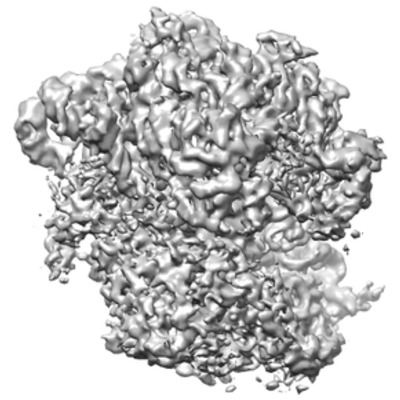
\includegraphics[width=0.45\textwidth]{Emd_8647.png}
\centering
\captionsetup{justification=centering}
\caption{Mycobacterium Smegmatis: Resolution 2.5 \AA }
\label{fig:EMD-8647-3d-struct}
\end{figure}

EMD-4138 (figure \ref{fig:EMD-4138-3d-struct}) is a \textbf{M}aedi-\textbf{V}isna \textbf{V}irus (MVV) intasome. It is having the resolution of $4.94\AA$ and the map dimension as $300\times300\times300$. Its map has a lot of extra empty padding in 3D, so one can use it directly or remove this empty padding. In our all experiments, cropped mapped is used rather than full map, so after cropping the dimension is $161\times161\times161$. 

\begin{figure}[H]
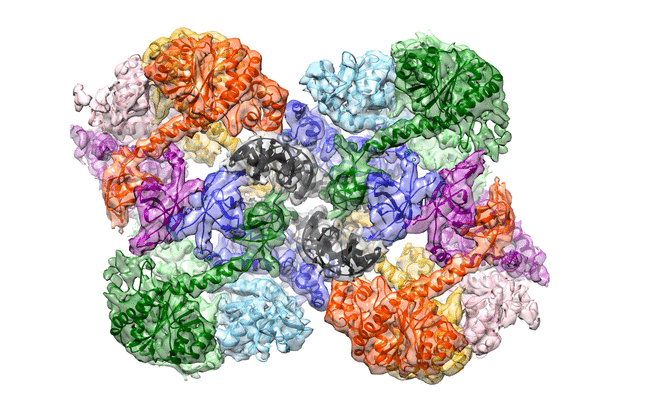
\includegraphics[width=0.5\textwidth]{Emd_4138.png}
\centering
\captionsetup{justification=centering}
\caption{Maedi-Visna Virus (MVV) intasome: Resolution 4.94 \AA }
\label{fig:EMD-4138-3d-struct}
\end{figure}

\subsection{Dataset Generation}

3D reconstruction is performed using the 2D projections taken from the EM, but as there is unavailability of EM or micrographs for  \& Mycobacterium Smegmatis \& Maedi-Visna Virus these digital EMD-8647 \& EMD-4138 have been used. For taking projections from EMD-8647 \& EMD-4138 computer simulated tool TIGRE (refer section \ref{subsec:TIGRE}) is used. Two types of dataset is being generated, i.e., one without any shifts in the projections and one with the shifts. Figure (\ref{subfg:emd_8647_proj1}) \& (\ref{subfg:emd_4138_proj1}]) shows the sample projection for  EMD-8647 \& EMD-4138 taken at the angles $[-35^{\circ} ,62^{\circ} -115^{\circ}]$ \& $[-86^{\circ},43^{\circ},50^{\circ}]$ respectively.  

\begin{figure}[h]
\centering
\begin{subfigure}{.5\textwidth}
\centering
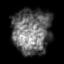
\includegraphics[width=0.8\linewidth]{Emd_8647_proj1.jpg}
\captionsetup{justification=centering}
\caption{ EMD-8647: A sample projection }
\label{subfg:emd_8647_proj1}
\end{subfigure} 
\begin{subfigure}{.48\textwidth}
\centering
\includegraphics[width=0.8\linewidth]{Emd_4138_proj_1.jpg}
\captionsetup{justification=centering}
\caption{ EMD-4138: A sample projection}
\label{subfg:emd_4138_proj1}
\end{subfigure}
\caption{2D Projections}
\label{fig:Emdb-2D-projections}
\end{figure}

The angles projections are taken from the i.i.d Gaussian distribution. So, a quternion is generated from Gaussian random generator then this quternion is converted into its angle representation.  All these projections are center aligned, i.e., they are having zero shift. But for experimenting ShARP algorithm, shifts have been added, and for ARP algorithm they are used as it is.  After that, a different level of noise is being added to these projections for testing the stability algorithms.

\subsubsection{Noise}

Projections taken from the EM are highly noisy. So, our proposed algorithm must be susceptible to noise. So to make that noise has been added explicitly to these non-noisy projections. The noise which is being added is the Gaussian noise with sigma as 10\%, 30\%, 50\%, 80\% \& 100\%  of the mean intensity of all the projections. So, a total of  6 datasets (including zero noise) have been generated per samples, and the tests have been performed on all these datasets. Figure (\ref{fig:EMD-8647 Projections: Noisy}) shows the sample projections all the 6 noise level for EMD-8647 and figure (\ref{fig:fig:EMD-4138 Projections: Noisy}) is for EMD-4138.


\begin{figure}[h]
\centering

\begin{subfigure}{.3\textwidth}
\centering
\includegraphics[width=0.8\linewidth]{Emd_8647_proj1.jpg}
\captionsetup{justification=centering}
\caption{ Noise 0\% }
\end{subfigure} 
\begin{subfigure}{.27\textwidth}
\centering
\includegraphics[width=0.8\linewidth]{Emd_8647_proj1_noise_10.jpg}
\captionsetup{justification=centering}
\caption{ Noise 10\%}
\end{subfigure}
\begin{subfigure}{.28\textwidth}
\centering
\includegraphics[width=0.8\linewidth]{Emd_8647_proj1_noise_30.jpg}
\captionsetup{justification=centering}
\caption{ Noise 30\%}
\end{subfigure}

\begin{subfigure}{.3\textwidth}
\centering
\includegraphics[width=0.8\linewidth]{Emd_8647_proj1_noise_50.jpg}
\captionsetup{justification=centering}
\caption{ Noise 50\% }
\end{subfigure} 
\begin{subfigure}{.27\textwidth}
\centering
\includegraphics[width=0.8\linewidth]{Emd_8647_proj1_noise_80.jpg}
\captionsetup{justification=centering}
\caption{ Noise 80\%}
\end{subfigure}
\begin{subfigure}{.28\textwidth}
\centering
\includegraphics[width=0.8\linewidth]{Emd_8647_proj1_noise_100.jpg}
\captionsetup{justification=centering}
\caption{ Noise 100\%}
\end{subfigure}
\caption{EMD-8647 Projections with no shift}
\label{fig:EMD-8647 Projections: Noisy}
\end{figure}


\begin{figure}[h]
\centering

\begin{subfigure}{.3\textwidth}
\centering
\includegraphics[width=0.8\linewidth]{Emd_4138_proj_1.jpg}
\captionsetup{justification=centering}
\caption{ Noise 0\% }
\end{subfigure} 
\begin{subfigure}{.27\textwidth}
\centering
\includegraphics[width=0.8\linewidth]{Emd_4138_proj1_noise_10.jpg}
\captionsetup{justification=centering}
\caption{ Noise 10\%}
\end{subfigure}
\begin{subfigure}{.28\textwidth}
\centering
\includegraphics[width=0.8\linewidth]{Emd_4138_proj1_noise_30.jpg}
\captionsetup{justification=centering}
\caption{ Noise 30\%}
\end{subfigure}

\begin{subfigure}{.3\textwidth}
\centering
\includegraphics[width=0.8\linewidth]{Emd_4138_proj1_noise_50.jpg}
\captionsetup{justification=centering}
\caption{ Noise 50\% }
\end{subfigure} 
\begin{subfigure}{.27\textwidth}
\centering
\includegraphics[width=0.8\linewidth]{Emd_4138_proj1_noise_80.jpg}
\captionsetup{justification=centering}
\caption{ Noise 80\%}
\end{subfigure}
\begin{subfigure}{.28\textwidth}
\centering
\includegraphics[width=0.8\linewidth]{Emd_4138_proj1_noise_100.jpg}
\captionsetup{justification=centering}
\caption{ Noise 100\%}
\end{subfigure}
\caption{EMD-4138 Projections with no shift}
\label{fig:EMD-4138 Projections: Noisy}
\end{figure}

\subsubsection{Shift}

Another set 6 datasets each sample in generated with the shift. First, the shift error is added to the projections, and then noise has been added. For EMD-8647 dataset, shift error added is between +/- 5 pixels in both x \& y direction taking the center of the image as the origin. For EMD-4138 dataset shift error is between +/-  10 pixels in both x and y-direction.

\subsection{Algorithm Pipeline}

This section talks about the complete reconstruction algorithm pipeline, i.e., combining all the modules discussed in this chapter until now. It is a serial pipeline where the output of any module will act as the input to its next module. If any of the modules are removed or replaced then final output will be affected drastically, for example replacing \textit{Angles Initialization} with random initialization.  

\begin{figure}[H]
\includegraphics[width=1\textwidth]{3d-reconstrction-pipepline.png}
\centering
\captionsetup{justification=centering}
\caption{3D-Reconstruction Pipeline }
\label{fig:3D-Reconstruction Pipeline}
\end{figure}

Pipeline (figure \ref{fig:3D-Reconstruction Pipeline}) has 5 stages, first is  \textit{Common line estimation}, second is  \textit{angle and shift initial estimation}, third is \textit{initial 3D reconstruction}, fourth is the \textit{Correlation Optimization} and  last is the \textit{final 3D reconstruction}. Almost all the stages take the projections as their input. The first stage takes the projections as the input to give the $\Phi$ matrix. This $\Phi$ matrix is given input to the second stage for the initial angles and shifts estimation for the projections. These initial estimates are used for initial 3D reconstruction in the third stage. The fourth stages takes projections $\boldsymbol{R_i^{init}}$, $\boldsymbol{S_i^{init}}$ \& $\boldsymbol{G^{init}}$ as the input for the optimization and the output are $\boldsymbol{R_i^{est}}$ \& $\boldsymbol{S_i^{est}}$. The fifth stage will use the output of the fourth stage for doing the final reconstruction. One thing to note here is that its a forward pipeline, i.e. no loops.

\subsection{Angle Recovery Problem: ARP} \label{subsec:ARP-EXP}

Angle recovery problem only considers the unknown angles into account and assumes that there is no shift. So the complete algorithm flow pipeline is mentioned in figure (\ref{fig:3D-Reconstruction Pipeline-ARP}) First, the common line is estimated using the given $N$ number of projections, which further gives $\Phi_{N\times N}$. This $\Phi$ is used for initial angles estimation using A. Singer methods (refer section \ref{subsec: angle_initialization}), which returns the rotation matrix in Euler XYZ convention. Using this $\boldsymbol{R_i^{init}}$ matrices initial 3D object $\boldsymbol{G^{init}}$ is reconstructed. Then $\boldsymbol{R_i^{init}}$ \& $\boldsymbol{G^{init}}$ are used for optimizing eq. (\ref{eq:our_obj_fun_arp}), which in returns gives the final 3D reconstructed object


\begin{figure}[H]
\includegraphics[width=1\textwidth]{3d-reconstrction-pipepline-ARP.png}
\centering
\captionsetup{justification=centering}
\caption{3D-Reconstruction Pipeline - ARP }
\label{fig:3D-Reconstruction Pipeline-ARP}
\end{figure}

This algorithm pipeline is tested on samples, i.e., EM-8647 \& EM-4138. The results for these datasets are mentioned below. These results try to compare original, initial reconstruction using A. Singer method and our 3D reconstructed object. 

\subsubsection{\textbf{EM-8647}}

EM-8647 is downsampled to $64\times64\times64$ before taking the projections. So, after taking the projections, the dimension of each projection is $64\times64$. Using the noiseless projections 5 more datasets are generated at different noise levels i.e. 10\%, 30\%, 50\% 80\% \& 100\%. Then the whole algorithm pipeline is tested on these 6 datasets. For removing the noise instead of clustering, BM3D for Gaussian noise removal is used (see section \ref{subsubsec:BM3D}).

Figure (\ref{fig:EMD-8647 Reconstruction: Result-noise 100}) shows the 3D reconstruction using the 500 projections with 100\% noisy dataset. Each row represents a slice of a 3D object of dimension $64\times64\times64$. Four rows are representing the four slices- 21, 34, 45 \& 48 in order. Each row has three columns, where the first column shows the true object slice, the second column shows the slice of $G^{init}$ and the third column shows the slice of $G^{est}$, i.e. our correlation result. 


\begin{figure}[H]
\centering

\begin{subfigure}{1\textwidth}
\centering
\includegraphics[width=1\linewidth]{emd_8647_result_1.png}
\captionsetup{justification=centering}
\caption{ Slice-21 }
\end{subfigure} 

\begin{subfigure}{1\textwidth}
\centering
\includegraphics[width=1\linewidth]{emd_8647_result_2.png}
\captionsetup{justification=centering}
\caption{ Slice-34 }
\end{subfigure} 

\begin{subfigure}{1\textwidth}
\centering
\includegraphics[width=1\linewidth]{emd_8647_result_3.png}
\captionsetup{justification=centering}
\caption{ Slice-45 }
\end{subfigure} 

\begin{subfigure}{1\textwidth}
\centering
\includegraphics[width=1\linewidth]{emd_8647_result_4.png}
\captionsetup{justification=centering}
\caption{ Slice-48 }
\end{subfigure} 


\caption{EMD-8647 reconstruction result for noise level 100\% with 500 projections}
\label{fig:EMD-8647 Reconstruction: Result-noise 100}
\end{figure}


One thing to note here is that the initial and final rotation estimate will not be the same as true rotation because all the estimated rotation will have some come global rotation which cannot be solved without knowing the true rotation. So, as these are the simulated experiments, the true rotations are known. Using these true rotations, the global rotation is calculated. Using that global rotation matrix both  $G^{init}$ \&  $G^{est}$ are aligned with the true  $G^{true}$ object so that comparison can be done easily.

\subsubsection{\textbf{Convergence Plot}}
Plot (\ref{figplot:emd_8647_result_Bm3d_convergence}) represents the convergence of the \textit{Correlation Optimization} eq. (\ref{eq:our_obj_fun_arp}) at every iteration. Y-axis represents the correlation \textit{error} (refer eq. (\ref{eq:our_arp_correaltion_error})) and the x-axis represent the iteration.

\begin{figure}[H]
\includegraphics[width=1\textwidth]{emd_8647_result_Bm3d_convergence.png}
\centering
\captionsetup{justification=centering}
\caption{EMD-8647: Convergence plot for reconstruction using 500 projections at 100\% noise level. }
\label{figplot:emd_8647_result_Bm3d_convergence}
\end{figure}

Table (\ref{tbl:our_arp_8647_result-2d-correlation}) shows the average 2D normalized correlation between the initial estimated projections and final estimated projections with the true projections. Correlation is represented by eq. (\ref{eq:our_arp_correaltion_error}). 
\begin{table}[H]
    \centering
     \begin{tabular}{||c c c c ||} 
             \hline
             Noise level & $NCor(P^{true},P^{init})$  &   $ NCor(P^{true},P^{est})$ & Iteration \\
            \hline\hline
            0\% & 0.980593 & 0.996572 & 18 \\
            \hline
            10\% &  0.980732 & 0.995853 & 20  \\
            \hline
            30\% &  0.980877 &  0.994158 & 20  \\
            \hline
            50\% & 0.978696 & 0.992373 & 20 \\
            \hline
            80\% & 0.969446 & 0.988164 & 20 \\
            \hline
            100\%& 0.960356 & 0.983171 & 20 \\
            \hline
    \end{tabular}
    \caption{EMD-8647: 2D normalized correlation of estimated projections using 500 projections with true projections }
    \label{tbl:our_arp_8647_result-2d-correlation}
\end{table}

\subsubsection{\textbf{Result}}

Estimated time for convergence is approximately 24 hours for the $\epsilon$  of 0.0001, $\epsilon$ represent change of error from previous iteration to current iteration. Table (\ref{tbl:our_arp_8647_result-3d-correlation}) represents the 3D normalized correlation (\textbf{NCor}) between initially reconstructed object $\boldsymbol{G^{int}}$ with the true object and the final reconstructed object $\boldsymbol{G^{est}}$ with true object at different noise levels. 

\begin{table}[H]
    \centering
     \begin{tabular}{||c c c||} 
             \hline
             Noise level & $ NCor(G^{true},G^{init})$  &  $NCor(G^{true},G^{est})$ \\
             \hline\hline
            0\%  & 0.870289 & 0.951389 \\
            \hline
            10\% & 0.839869 & 0.920174	 \\
            \hline
            30\% & 0.811552 & 0.875694    \\
            \hline
            50\% & 0.781301 & 0.841529 \\
            \hline
            80\% & 0.741130 & 0.807155 \\
            \hline
            100\%& 0.716864 & 0.788950 \\[1ex] 
            \hline
    \end{tabular}
    \captionsetup{justification=centering}
    \caption{EMD-8647: 3D normalized correlation of the reconstructed object using 500 projections with true object }
    \label{tbl:our_arp_8647_result-3d-correlation}
\end{table}

\subsubsection{\textbf{EM-4138}}

EM-4138 original map dimension is $300\times300\times300$  with lots of empty background space. So for experiments, it is cropped to $161\times161\times161$ before taking the projections. So, after taking the projections, the dimension of each projection is $161\times161$. Using the noiseless projections, 5 more datasets are generated at different noise levels i.e. 10\%, 30\%, 50\% 80\% \& 100\%. Then the whole algorithm pipeline is tested on these 6 datasets. For removing the noise instead of clustering, BM3D for Gaussian noise removal is used (see section \ref{subsubsec:BM3D}). 

Figure (\ref{fig:EMD-4138 Reconstruction: Result-noise 100}) shows the 3D reconstruction using the 500 projections with 100\% noisy dataset. Each row represents a slice of a 3D object of dimension $161\times161\times161$. Four rows are representing the four slices- 59, 67, 82 \& 89 in order. Each row has three columns, where the first column shows the true object slice, the second column shows the slice of $G^{init}$ and the third column shows the slice of $G^{est}$, i.e., our correlation result.

\begin{figure}[H]
\centering

\begin{subfigure}{1\textwidth}
\centering
\includegraphics[width=1\linewidth]{emd_4138_result_1.png}
\captionsetup{justification=centering}
\caption{ Slice-59 }
\end{subfigure} 

\begin{subfigure}{1\textwidth}
\centering
\includegraphics[width=1\linewidth]{emd_4138_result_2.png}
\captionsetup{justification=centering}
\caption{ Slice-67 }
\end{subfigure} 

\begin{subfigure}{1\textwidth}
\centering
\includegraphics[width=1\linewidth]{emd_4138_result_3.png}
\captionsetup{justification=centering}
\caption{ Slice-82 }
\end{subfigure} 

\begin{subfigure}{1\textwidth}
\centering
\includegraphics[width=1\linewidth]{emd_4138_result_4.png}
\captionsetup{justification=centering}
\caption{ Slice-89 }
\end{subfigure} 
\captionsetup{justification=centering}
\caption{EMD-4138 reconstruction result for noise level 100\% with 500 projections}
\label{fig:EMD-4138 Reconstruction: Result-noise 100}
\end{figure}

\subsubsection{\textbf{Convergence Plot}}

Plot (\ref{figplot:emd_4138_result_Bm3d_convergence}) represents the convergence of the \textit{Correlation Optimization} eq. \ref{eq:our_obj_fun_arp} at every iteration. Y-axis represents the correlation \textit{error} (refer eq. [\ref{eq:our_arp_correaltion_error}]) and the x-axis represents the iteration.

\begin{figure}[H]
\includegraphics[width=1\textwidth]{emd_4138_result_Bm3d_convergence.png}
\centering
\captionsetup{justification=centering}
\caption{EMD-4138: Convergence plot for reconstruction using 500 projections at 100\% noise level. }
\label{figplot:emd_4138_result_Bm3d_convergence}
\end{figure}

Table (\ref{tbl:our_arp_4138_result-2d-correlation}) shows the average 2D normalized correlation between the initial estimated projections and final estimated projections with the true projections. Correlation is represented by eq. (\ref{eq:our_arp_correaltion_error}). 
\begin{table}[H]
    \centering
     \begin{tabular}{||c c c c ||} 
             \hline
             Noise level & $ NCor(P^{true},P^{init})$  &   $ NCor(P^{true},P^{est})$ &  Iteration \\
             \hline\hline
             0\% & 0.992866  & 0.995287 & 13 \\
            \hline
            10\% & 0.992235  & 0.995002 & 13 \\
            \hline
            30\% &0.988352  & 0.993723 & 11  \\
            \hline
            50\% &0.981935  & 0.992033 & 19 \\ 
            \hline
            80\% &0.968330  & 0.988639 & 12 \\
            \hline
            100\% &0.906425  & 0.941335 & 18 \\ [1ex]
            \hline
    \end{tabular}
    \captionsetup{justification=centering}
    \caption{EMD-4138: 2D normalized correlation of estimated projections using 500 projections with true projections }
    \label{tbl:our_arp_4138_result-2d-correlation}
\end{table}

\subsubsection{\textbf{Result}}

Estimated time for convergence is approximately 48 hours for the $\epsilon$  of 0.00001, $\epsilon$ represent change of error from previous iteration to current iteration. Table \ref{tbl:our_arp_4138_result-3d-correlation} represents the 3D normalized correlation (\textbf{NCor}) between initially reconstructed object $\boldsymbol{G^{int}}$ with the true object and the final reconstructed object $\boldsymbol{G^{est}}$ with true object at different noise levels. 

\begin{table}[H]
    \centering
     \begin{tabular}{||c c c||} 
             \hline
             Noise level & $NCor(G^{true},G^{init})$  &  $NCor(G^{true},G^{est})$ \\ 
             \hline\hline
             0\% & 0.948375 & 0.964472 \\
             \hline
             10\% & 0.943699 & 0.959397 \\
             \hline
             30\% & 0.920251 & 0.946016 \\
             \hline
             50\% & 0.890837 & 0.932847 \\
             \hline
             80\% & 0.840490 & 0.912345 \\
             \hline
             100\% & 0.726130 & 0.823344 \\ [1ex] 
             \hline
    \end{tabular}
    \captionsetup{justification=centering}
    \caption{EMD-4138: 3D normalized correlation of the reconstructed object using 500 projections with true object }
    \label{tbl:our_arp_4138_result-3d-correlation}
\end{table}

Table (\ref{tbl:our_arp_4138_result-acos-rot}) shows the final orientation error between the estimated and true orientation. In table \ref{tbl:our_arp_4138_result-acos-rot}, $r_1,r_2 \& r_3$ represents the first,second and third column vector of the rotation matrix respectively. Columns of the table shows the average initial and estimated orientation error for 500 projection. For 100\% noise level initial orientation error is approx. $10^\circ, 8.7^\circ \& 12.1^\circ$ and our estimated orientation is $4^\circ,5.3^\circ \& 0.01^\circ$. 

\begin{table}[H]
    \centering
     \begin{tabular}{||c c c c c||} 
             \hline
             Noise 
             & $acos(r_1^{t},r_1^{init})$ 
             & $acos(r_1^{t},r_1^{est})$
             & $acos(r_2^{t},r_3^{init})$ 
             & $acos(r_2^{t},r_3^{est})$
            \\ 
            \hline\hline
            0\%  &1.457517&0.478219&1.434820 &0.616686\\ \hline
            10\% &1.557083&0.519157&1.510970 &0.683813\\ \hline
            30\% &2.465120&0.803880&2.435245 &1.155705\\ \hline
            50\% &3.730979&0.912525&3.352269 &1.113716\\ \hline
            80\% &6.805973&2.031066&6.021201 &2.831163\\ \hline
            100\%&10.07483&4.150101&8.741050 &5.350236\\ \hline
            \hline
    \end{tabular}
    \begin{tabular}{||c c c||} 
             \hline
             Noise 
             & $acos(r_3^{t},r_3^{init})$ 
             & $acos(r_3^{t},r_3^{est})$
            \\ 
            \hline\hline
            0\%  &1.988203&0.001233\\ \hline
            10\% &2.008021&0.001362\\ \hline
            30\% &3.000396&0.002302\\ \hline
            50\% &4.054885&0.002219\\ \hline
            80\% &8.076550&0.005640\\ \hline
            100\%&12.07059&0.010658\\ \hline
            \hline
    \end{tabular}
    \captionsetup{justification=centering}
    \caption{EMD-4138:Final errors in degrees between estimated and correct orientation}
    \label{tbl:our_arp_4138_result-acos-rot}
\end{table}

\subsection{Shift-Angle Recovery Problem: ShARP}\label{subsec:ShARP-EXP}

ShARP do not assume anything on shifts, i.e., the shift can be there or cannot.  Pipeline (\ref{fig:3D-Reconstruction Pipeline-Sharp}) is  little modified version of pipeline shown in figure (\ref{fig:3D-Reconstruction Pipeline}). As till now, in our experiments stage 1\&  2 problems are not solved for shifted projections. So,  $S_i^{init}$ can't be predicted right now and this the part of the future work. So for testing our ShARP algorithm (\ref{algo:our_sharp}) the architecture \ref{fig:3D-Reconstruction Pipeline} has been modified to new architecture \ref{fig:3D-Reconstruction Pipeline-Sharp}. In this modified architecture, common line and initial angles estimate performed on projections with \textit{no shift}, i.e., stage 1, 2 \& 3. For the later stages \textit{shifted} projections are used, i.e. stage 4 \& 5. Once shift estimation problems for stage 1 \& 2 are solved then architecture \ref{fig:3D-Reconstruction Pipeline} can be used directly.

\begin{figure}[H]
\includegraphics[width=1\textwidth]{3d-reconstrction-pipepline-Sharp.png}
\centering
\captionsetup{justification=centering}
\caption{3D-Reconstruction Pipeline }
\label{fig:3D-Reconstruction Pipeline-Sharp}
\end{figure}

\subsubsection{\textbf{EM-8647}}
EM-8647 is downsampled to $64\times64\times64$ before taking the projections. So, after taking the projections, the dimension of each projection is $64\times64$. Then random shift between -5 to 5 pixels in both x and y directions are added onto these projections. After that, using the noiseless shifted projections, five more datasets are generated at different noise levels, i.e., 10\%, 30\%, 50\% 80\% \& 100\%. Then the whole algorithm pipeline is tested on these 6 datasets. For removing the noise instead of clustering, BM3D for Gaussian noise removal is used (see section \ref{subsubsec:BM3D}). Rotation search space hyperparameter $k$ is set to +/-10 degree.

Figure (\ref{fig:EMD-8647 Reconstruction: Result-noise-100-shift-5}) shows the 3D reconstruction using the 500 shifted projections with 100\% noisy dataset. Each row represents a slice of a 3D object of dimension $64\times64\times64$. Four rows are representing the four slices- 22, 28, 34 \& 49 in order. Each row has two columns, where the first column shows the true object slice, and the second column shows the slice of $G^{est}$, i.e., our correlation result. 

\begin{figure}[H]
\centering

\begin{subfigure}{1\textwidth}
\centering
\includegraphics[width=0.8\linewidth]{emd_8647_result_sharp_1.png}
\captionsetup{justification=centering}
\caption{ Slice-22 }
\end{subfigure} 

\begin{subfigure}{1\textwidth}
\centering
\includegraphics[width=0.8\linewidth]{emd_8647_result_sharp_2.png}
\captionsetup{justification=centering}
\caption{ Slice-28 }
\end{subfigure} 

\begin{subfigure}{1\textwidth}
\centering
\includegraphics[width=0.8\linewidth]{emd_8647_result_sharp_3.png}
\captionsetup{justification=centering}
\caption{ Slice-34 }
\end{subfigure} 

\begin{subfigure}{1\textwidth}
\centering
\includegraphics[width=0.8\linewidth]{emd_8647_result_sharp_4.png}
\captionsetup{justification=centering}
\caption{ Slice-49 }
\end{subfigure} 
\captionsetup{justification=centering}
\caption{EMD-8647 reconstruction result for noise level 100\%  with 500 projections having random shift from -5 to 5 pixels in both x and y direction}
\label{fig:EMD-8647 Reconstruction: Result-noise-100-shift-5}
\end{figure}

\subsubsection{Conversion Plot}

Plot (\ref{figplot:emd_8647_result_shift-Bm3d_convergence}) represents the convergence of the \textit{Correlation Optimization} eq. \ref{eq:our_obj_fun_sharp} at every iteration. Y-axis represents the correlation \textit{error} (refer eq. [\ref{eq:our_sharp_correaltion_error}]) and the x-axis represents the iteration.

\begin{figure}[H]
\includegraphics[width=1\textwidth]{emd_8647_result_shift_5_Bm3d_convergence.png}
\centering
\captionsetup{justification=centering}
\caption{EMD-8647: Convergence plot for reconstruction using 500  projections randomly shifted from -5 to 5 pixels in both x and y direction at 100\% noise level. }
\label{figplot:emd_8647_result_shift-Bm3d_convergence}
\end{figure}



Table (\ref{tbl:our_shapr_8647_result-2d-correlation}) shows the average 2D normalized correlation between the initial estimated projections and final estimated projections with the true projections. Correlation is represented by eq. [\ref{eq:our_arp_correaltion_error}]. 

\begin{table}[H]
    \centering
     \begin{tabular}{||c c c ||} 
             \hline
             Noise level & $ NCor(P^{true},P^{est})$ &  Iteration \\
             \hline\hline
            0\%   &0.996562 & 20 \\ \hline
            10\%  &0.995828 & 10 \\ \hline
            30\%  &0.994116 & 20 \\ \hline
            50\%  &0.992103 & 20 \\ \hline
            80\%  &0.987488 & 20 \\ \hline
            100\% &0.983475 & 20 \\ \hline
            \hline
    \end{tabular}
    \caption{EMD-8647: 2D normalized correlation of estimated projections using 500 projections with true projections }
    \label{tbl:our_shapr_8647_result-2d-correlation}
\end{table}

\subsubsection{\textbf{Result}}

Estimated time for convergence is approximately 24 hours using one CPU and GPU for the $\epsilon$  of 0.00001, $\epsilon$ represent change of error from previous iteration to current iteration. Table \ref{tbl:our_sharp_8674_result-3d-correlation} represents the 3D normalized correlation (\textbf{NCor}) between final reconstructed object $\boldsymbol{G^{int}}$ with the true object and it's \textit{relative RMS} at different noise levels. 

\begin{table}[H]
    \centering
     \begin{tabular}{||c c c||} 
             \hline
             Noise level & $NCor(G^{true},G^{init})$  &  Relative RMS \\ 
             \hline\hline
            0\%   &0.935679 & 0.948323 \\\hline
            10\%  &0.919888 & 0.953236 \\\hline 
            30\%  &0.875297 & 0.957525 \\\hline
            50\%  &0.840329 & 0.962327 \\\hline
            80\%  &0.805708 & 0.970887 \\\hline
            100\% &0.789092 & 0.975451 \\\hline
             \hline
    \end{tabular}
    \captionsetup{justification=centering}
    \caption{EMD-8647: 3D normalized correlation of the reconstructed object using 500 projections with true object }
    \label{tbl:our_sharp_8674_result-3d-correlation}
\end{table}


Table (\ref{tbl:our_sharp_8647_result-acos-rot}) shows the final orientation error between the estimated and true orientation. In table (\ref{tbl:our_sharp_8647_result-acos-rot}), $r_1,r_2 \& r_3$ represents the first,second and third column vector of the rotation matrix respectively. Columns of the table shows the average estimated orientation error for 500 projection. For 100\% noise level our estimated orientation is $6.2^\circ,10.4^\circ \& 0.02^\circ$. 

\begin{table}[H]
    \centering
     \begin{tabular}{||c c c c||} 
             \hline
             Noise 
             & $acos(r_1^{t},r_1^{est})$ 
             & $acos(r_2^{t},r_2^{est})$
             & $acos(r_3^{t},r_3^{est})$ 
             \\ 
            \hline\hline
            0\%   &0.380730&0.425491&0.000851 \\\hline
            10\%  &0.395875&0.447099&0.000891 \\\hline
            30\%  &0.495726&0.584583&0.001165 \\\hline
            50\%  &0.798299&0.948386&0.001889 \\\hline
            80\%  &2.872667&5.175899&0.010311 \\\hline
            100\% &6.287650&10.474817&0.02086 \\\hline
            \hline
    \end{tabular}
    \captionsetup{justification=centering}
    \caption{EMD-8647: Final orientation errors in degrees between estimated and correct rotation matrix}
    \label{tbl:our_sharp_8647_result-acos-rot}
\end{table}

Table (\ref{tbl:our_sharp_8647_result-trans-error}) shows the final shift error, i.e., by how much predicted shifts are far from the true shifts. The table shows the means shift error for all the 500 projections and also the standard deviation. As one can see that for 0\%,10\% \& 30\% noise level, the mean shifts errors are zero, meaning the predicted shifts matches exactly with the true shifts. Here, shifts are found out using the cross-power spectrum method. 

\begin{table}[H]
    \centering
     \begin{tabular}{||c|c|c|c|c||} 
             \hline
            \multirow{2}{*}{Noise} 
             & \multicolumn{2}{c|}{Mean} 
             & \multicolumn{2}{c|}{$\sigma$} \\
             \cline{2-5}
             & X-axis & Y-Axis & X-axis & Y-Axis\\
            \hline\hline
            0\%   & 0 & 0 & 0 & 0 \\\hline
            10\%  &0 & 0 & 0 & 0 \\\hline
            30\%  &0 & 0 & 0 & 0 \\\hline
            50\%  &0.001992 & 0.001992 & 0.044632 & 0.044632 \\\hline
            80\%  &0.029880 & 0.013944 & 0.230212 & 0.204258 \\\hline
            100\% &0.033865 & 0.049801 & 0.276939 & 0.315137 \\\hline
            \hline
    \end{tabular}
    \captionsetup{justification=centering}
    \caption{EMD-8647: Mean and Standard deviation of shift in pixels between estimated and true projection shifts}
    \label{tbl:our_sharp_8647_result-trans-error}
\end{table}

\subsection{Conclusion}

Experiments performed for testing ARP (see section \ref{subsec:ARP-EXP}) and ShARP (see section \ref{subsec:ShARP-EXP}) algorithm and the complete pipeline shows the promising results. Considering ARP, the final 3D normalized correlation is higher than the initial one, which is computed using the A. Singer et al. \cite{singer2009threeAngleEstimate}. It means running our algorithm (see [\ref{algo:our_arp}]) after the A.Singers et. al \cite{singer2009threeAngleEstimate} method will give the more precise estimation. \\

As shown, ShARP experiments see section (\ref{subsec:ShARP-EXP})), finding shifts using cross-power spectrum works best instead of doing the doing brute force in x and y-axis. Also, the brute force method will increase one more hyperparameter specifying the 2D search shift space, similar to the rotation hyperparameter.  \\

Estimated execution time ARP and ShARP algorithm with one GPU is approximately 24 hrs for 500 projections of dimension $64x64$ and approximately 48 hrs for 500 projections of dimension $161x161$. Inner loop of the ARP algorithm (\ref{algo:our_arp}) and ShARP algorithm (\ref{algo:our_sharp}) can be parallelized using multiple GPUs. As this will reduce the execution time drastically, i.e., even with two GPU cards time will reduce to half. Currently, all our experiments are performed on a single Nvidia Quadro M4000 GPU device. 

\chapter{Future work}

\section{Particle Picking}
Our experiments show that using the classifiers SVM, Random Forest, and Faster R-CNN, the translation error is between 20 to 40 pixels. Translation error denotes displacement from its true center. This translation error will create a problem at the time of 3D reconstruction. So, for testing 3D reconstruction accuracy, third-party software like Imagic, Eman, Relion, Cryo-Sparc, etc. or our proposed algorithm (section \ref{sec: Proposed_Algorithm}) can be used. That will help in deciding how precisely the model can mark out the particles on micrograph.\\

 Micrograph generated for a biological sample from cryo-em has low SNR value. So, training classifier from very noisy data will give less accuracy. In our experiments, denoising of the micrographs was not handled.  So one way to handle noisy data is to first denoise the train set and then train the model.\\

For training classifiers, SVM and Random Forest directly on raw image pixels are not advisable because 100x100 image will have 10K pixels, i.e., features and training on 10K feature will take too much time. Also, a large amount of training data is required for correct classification. So, in our experiments, PCA was used for reducing the dimension of the image, then the reduced dimensions were treated as features for training classifier. For reducing dimension, \textit{Auto-Encoder}  (deep learning based model) \cite{meng2017relational} can also be used, but Auto-Encoder also requires separate training. Also, Random Forest classifier is a CPU based algorithm because of that time of detection is very large, if Random Forest is implemented on GPU, then its detection time can be reduced drastically.\\

In Faster R-CNN experiment, about 15K particles were used for training. Next thing that can be done is to design new CNN architecture so that the number of marks required for training is less. Because if a model is trained with less markings and it gives good accuracy then that model will be considered best compare to other one which require a large amount of data. In Cryo-EM, getting a large amount of data means manually marking those many particles, which require a large amount of time and effort whereas our final objective is to reduce this time and efforts.\\


\section{3D Reconstruction}

Execution time of ARP algorithm (\ref{algo:our_arp}) and ShARP algorithm (\ref{algo:our_arp}) with 500 projections and rotation search space hyperparameter as $+/- 10^{\circ}$ takes days for reconstruction using single GPU. So, if the algorithm is made parallelized for multiple GPU cards, then there will be a huge reduction in reconstruction time. These algorithms converge fast if the initial estimate is good, but if the initial estimate is bad, then this will also increase the convergence time. So, stage 2 for the algorithm pipeline (figure \ref{fig:3D-Reconstruction Pipeline}) should be good. \\

The ShARP algorithm pipeline (figure \ref{fig:3D-Reconstruction Pipeline-Sharp}) is modified a little bit, as problem for stage 1 \&  2 are not solved for the initial shift estimation. So, once the stage 1 \&  2 shift estimation problem is solved, then the ideal algorithm pipeline (figure \ref{fig:3D-Reconstruction Pipeline}) can be used instead of  ShARP algorithm pipeline. After then our code can be tested on the real projections taken from EM rather than simulated ones.\\

All the experiments are performed on simulated projections, but not on the real projections. Until algorithms  (ARP \& SHARP) are not tested on real projections, it cannot be used practical purpose. Also, real projections have few extra problems than need to be taken care of first before feeding it to our algorithm pipeline (figure \ref{fig:3D-Reconstruction Pipeline}). Our simulated non-noisy projections had background pixel value as zero, but this is not the case with the real projections. Real projections have ice (with noise) as there background, so this icy background has to be removed first. Next problem is less contrast, so CTF correction is needed before any use.
Another major problem is the Poisson noise. Currently, in our simulated experiments, Gaussian noise is added, and for removing it, BM3D for Gaussian noise is used. But for dealing noise for the real projections, either BM3D for Poisson noise should be used or clustering. After doing all the major pre-processing of real projections, then only they have to be fed in our algorithm pipeline.    













%****************************************************************
%                         Appendices                           
%****************************************************************
%% Additional, supporting material, such as codes, derivations, etc., can be placed in the appendix
%\appendix
%\chapter{Supporting Material}

%******************************************************************
%                         Bibliography or References          
%******************************************************************  
\bibliographystyle{plain}
\bibliography{ref}     


%*******************************************************************
%                        Acknowledgements                    
%******************************************************************* 
%%%
\acknowledgments

I would like to thank Sunil Vichare, Technical Officer and Ninad N. Shaha, Technical Superintendent of Computer Center, IIT Bombay for there constant support with hardware and internet bandwidth.  As, these datasets are in a few hundred GBs, so to download datasets large disk and bandwidth are required. CSE-Sysad, IIT Bombay has also helped us with the hardware support. More important, I would like thank VIGIL lab, IIT Bombay for providing voxel servers with GPUs. Without any GPU machine, completing this dissertation was near to impossible       


\signature{\today}
%\signature[Indian Institute of Technology Bombay]{\today}

%========================================================================

%%% Local Variables: 
%%% mode: latex
%%% TeX-master: "../mainrep"
%%% End:            

\end{document}